\documentclass{amsart}

\usepackage{amssymb}
\usepackage{graphicx}
\usepackage{enumerate}
\usepackage[dvipsnames]{xcolor}
\usepackage[pagebackref]{hyperref}
\hypersetup{
    colorlinks=true,
    linkcolor=blue,
    filecolor=blue,      
    urlcolor=blue, 
    citecolor=blue,
}
\usepackage{amsmath,amssymb,amsrefs}
\usepackage{tikz}
\usetikzlibrary{positioning, cd, arrows, backgrounds, arrows.meta,decorations,decorations.pathreplacing}
\usepackage{enumerate}
\usepackage{bm}
\usepackage{float}
\usepackage{wrapfig}
\usepackage{caption}
\usepackage{subcaption}
\usepackage{mathrsfs}
\usepackage{bbold}
\usepackage{appendix}
\usepackage{afterpage}
\usepackage{wasysym}
\usepackage{longtable}
\usepackage{stmaryrd}

\newcommand{\tin}{:}
\renewcommand{\ae}{\acute{e}}

\usetikzlibrary{nfold}

\tikzset{Rightarrow/.style={double distance=2pt,scaling nfold=2,>={Implies},->}}

\makeatletter
\newcommand{\oset}[3][0ex]{\mathrel{\mathop{#3}\limits^{
    \vbox to#1{\kern-2\ex@
    \hbox{$\scriptstyle#2$}\vss}}}}
\makeatother
\newcommand{\Cat}[1]{\mathsf{#1}}
\newcommand{\cat}[1]{\Cat{#1}}
\newcommand{\acat}[1]{\mathsf{#1}}

\newcommand{\Caps}[1]{\mathsf{#1}}


\newcommand{\smalltriangle}{\text{\scalebox{0.8}{$\triangle$}}}


\newcommand{\Core}[1]{\oset{\leftrightarrow}{\acat{#1}}}
\newcommand{\core}[1]{\Core{#1}}
\newcommand{\LongCore}[1]{\oset{\longleftrightarrow}{\acat{#1}}}
\newcommand{\lcore}[1]{\LongCore{#1}}
\DeclareRobustCommand\longtwoheadrightarrow
     {\relbar\joinrel\twoheadrightarrow}
\newcommand{\Epi}[1]{\oset{\twoheadrightarrow}{\acat{#1}}}
\newcommand{\epi}[1]{\Epi{#1}}
\newcommand{\LongEpi}[1]{\oset{\longtwoheadrightarrow}{\acat{#1}}}
\newcommand{\lepi}[1]{\LongEpi{#1}}  

\newcommand{\Mono}[1]{\oset{\hookrightarrow}{\acat{#1}}}
\newcommand{\mono}[1]{\Mono{#1}}
\newcommand{\NaN}{\Xi}

\captionsetup[subfigure]{labelfont=rm}


\usepackage[many]{tcolorbox}
\tcbuselibrary{listings}


\newlength\inwd
\setlength\inwd{1.3cm}
\newcounter{notebookcounter}


\newfloat{lstfloat}{htbp}{lop}
\floatname{lstfloat}{Listing}
\numberwithin{lstfloat}{section}

\colorlet{inputcolor}{blue!50!black}
\colorlet{outputcolor}{red!50!black}

\lstdefinelanguage{genericnotebookno}{
    morekeywords={print, def, return},
    morecomment=[l]{//},
    basicstyle=\footnotesize\ttfamily,
    keywordstyle=\color{green!40!black}\bfseries,
    commentstyle=\color{purple!40!black}\itshape,
}

\lstdefinelanguage{genericnotebookin}{
    morekeywords={print, def, return},
    morecomment=[l]{//},
    basicstyle=\footnotesize\ttfamily,
    keywordstyle=\color{green!40!black}\bfseries,
    commentstyle=\color{purple!40!black}\itshape,
}

\lstdefinelanguage{genericnotebookout}{
    morekeywords={:,Type},
    morecomment=[l]{//},
    basicstyle=\footnotesize\ttfamily,
    keywordstyle=\bfseries\color{green!40!black},
    commentstyle=\itshape\color{purple!40!black},
}

\newtcblisting{notebookno}[1][\thenotebookcounter]{
  enlarge left by=\inwd-1.2cm,
  width=\linewidth-\inwd,
  enhanced,
  boxrule=0.4pt,
  colback=ForestGreen!15,
  listing only,
  top=0pt,
  bottom=0pt,
  overlay={
    \node[
      anchor=north east,
      text width=\inwd,
      font=\footnotesize\ttfamily\color{inputcolor},
      inner ysep=2mm,
      inner xsep=0pt,
      outer sep=0pt
      ] 
      at (frame.north west)
      {\stepcounter{notebookcounter}};
  }
  listing engine=listing,
  listing options={
    aboveskip=1pt,
    belowskip=1pt,
    language=genericnotebookno,
    showstringspaces=false,
    breaklines=true,
  },
}

\newtcblisting{notebookin}[1][\thenotebookcounter]{
  enlarge left by=\inwd,
  width=\linewidth-\inwd,
  enhanced,
  boxrule=0.4pt,
  colback=ForestGreen!15,
  listing only,
  top=0pt,
  bottom=0pt,
  overlay={
    \node[
      anchor=north east,
      text width=\inwd,
      font=\footnotesize\ttfamily\color{inputcolor},
      inner ysep=2mm,
      inner xsep=0pt,
      outer sep=0pt
      ] 
      at (frame.north west)
      {\stepcounter{notebookcounter}In [#1]:};
  }
  listing engine=listing,
  listing options={
    aboveskip=1pt,
    belowskip=1pt,
    language=genericnotebookin,
    showstringspaces=false,
    breaklines=true,
  },
}
\newtcblisting{notebookout}[1][\thenotebookcounter]{
  enlarge left by=\inwd,
  width=\linewidth-\inwd,
  enhanced,
  boxrule=0.1pt,colback=White,
  listing only,
  top=0pt,
  bottom=0pt,
  overlay={
    \node[
      anchor=north east,
      text width=\inwd,
      font=\footnotesize\ttfamily\color{outputcolor},
      inner ysep=2mm,
      inner xsep=0pt,
      outer sep=0pt
      ] 
      at (frame.north west)
      {Out [#1]:};
  }
  listing engine=listing,
  listing options={
    aboveskip=1pt,
    belowskip=1pt,
    language=genericnotebookout,
    showstringspaces=false,
  },
}



\floatstyle{ruled}
\newfloat{typefloat}{htbp}{lop}
\floatname{typefloat}{Type}



\DeclareMathOperator{\enc}{enc}
\DeclareMathOperator{\cod}{code}
\DeclareMathOperator{\dec}{dec}
\DeclareMathOperator{\fun}{fun}
\DeclareMathOperator{\map}{map}
\DeclareMathOperator{\ab}{abel}
\DeclareMathOperator{\comm}{comm}
\DeclareMathOperator{\Cov}{Cov}
\DeclareMathOperator{\coim}{coim}
\DeclareMathOperator{\Cod}{Cod}
\DeclareMathOperator{\Adj}{Adj}
\DeclareMathOperator{\Isom}{Isom}
\DeclareMathOperator{\Dom}{Dom}
\DeclareMathOperator{\Codom}{Codom}
\DeclareMathOperator{\im}{Im}
\DeclareMathOperator{\sub}{sub}
\DeclareMathOperator{\Ker}{Ker}

\newcommand{\Free}[2]{#1\langle #2\rangle}
\DeclareMathOperator{\Residue}{Res}
\DeclareMathOperator{\Rad}{Rad}
\DeclareMathOperator{\Forget}{Frgt}
\DeclareMathOperator{\Fit}{Fit}

\DeclareMathOperator{\soc}{Soc}
\DeclareMathOperator{\End}{End}
\DeclareMathOperator{\Aut}{Aut}
\DeclareMathOperator{\Sym}{Sym}
\DeclareMathOperator{\GL}{GL}
\DeclareMathOperator{\Sp}{Sp}
\DeclareMathOperator{\GSp}{GSp}
\DeclareMathOperator{\PG}{PG}
\DeclareMathOperator{\iso}{Iso}
\DeclareMathOperator{\Iso}{Iso}
\DeclareMathOperator{\Hom}{Hom}
\DeclareMathOperator{\Span}{Span}
\DeclareMathOperator{\Cent}{Cent}
\DeclareMathOperator{\Der}{Der}
\DeclareMathOperator{\Stab}{\mathsf{Stab}}
\DeclareMathOperator{\Trap}{\mathsf{Trap}}
\DeclareMathOperator{\St}{\mathsf{St}}
\DeclareMathOperator{\Trans}{\mathsf{Trans}}
\DeclareMathOperator{\id}{id}
\DeclareMathOperator{\gl}{\mathfrak{gl}}
\DeclareMathOperator{\mychar}{char}
\DeclareMathOperator{\ftor}{Mor}

\newcommand{\srcfunc}{\mathbin{\blacktriangleleft}}
\newcommand{\tgtfunc}{\mathbin{\blacktriangleleft}}
\newcommand{\src}[1]{#1\srcfunc}
\newcommand{\tgt}[1]{\tgtfunc #1}

\DeclareMathOperator{\ob}{ob }
\usepackage{amsfonts}
\makeatletter
\def\amsbb{\use@mathgroup \M@U \symAMSb}
\makeatother
\newcommand{\one}{\mathbb{1}}
\newcommand{\N}{\mathbb{N}}
\newcommand{\Z}{\mathbb{Z}}
\newcommand{\F}{\mathbb{F}}
\renewcommand{\ker}{{\rm ker\,}}
\newcommand{\coker}{{\rm coker\,}}
\renewcommand{\hom}{\Hom}
\newcommand{\bmto}{\rightarrowtail}
\newcommand{\type}[1]{#1}
\tikzcdset{
  cells={font=\everymath\expandafter{\the\everymath\displaystyle}},
}

\newcommand{\East}{\mathrm{East}}
\newcommand{\EAST}{\East}
\newcommand{\homtype}{Hom} \newcommand{\valence}{\mathrm{val}}
\newcommand{\SLP}{\type{SLP}}
\usepackage{scalerel}  
\newcommand{\defeq}{\mathrel{\hstretch{.13}{=}\hspace{.2ex}{=}}}
\renewcommand{\leq}{\leqslant}
\renewcommand{\geq}{\geqslant}
\newcommand{\opp}[1]{(#1)}
\newcommand{\opb}[1]{[#1]}
\newcommand{\opbb}[1]{\llbracket #1\rrbracket}
\newcommand{\blank}{
    \,
\begin{tikzpicture}
        \draw[line width=0.5pt, draw=black, fill=gray!20] (0,0) rectangle (0.25,0.25);
    \end{tikzpicture}\,
}
\newcommand{\blanktwo}{
    \,
\begin{tikzpicture}
        \draw[line width=0.5pt, draw=black, fill=gray!20] (0,0) -- (0.3,0) -- (0.15,1.5/6) -- (0,0);
    \end{tikzpicture}\,
}
\newcommand{\inputref}[2]{\hyperref[#1]{\texttt{{\color{inputcolor}In\,[#2]}}}}
\newcommand{\outputref}[2]{\hyperref[#1]{\texttt{{\color{outputcolor}Out\,[#2]}}}}
\newcommand{\var}{{\rm var}}
\newcommand{\eval}{{\rm eval}}

\makeatletter
\newcommand{\xRrightarrow}[2][]{\ext@arrow 0359\Rrightarrowfill@{#1}{#2}}
\newcommand{\Rrightarrowfill@}{\arrowfill@\equiv\equiv\Rrightarrow}
\newcommand{\xLleftarrow}[2][]{\ext@arrow 3095\Lleftarrowfill@{#1}{#2}}
\newcommand{\Lleftarrowfill@}{\arrowfill@\Lleftarrow\equiv\equiv}
\makeatother

\newcommand{\hookdoubleheadrightarrow}{\hookrightarrow\mathrel{\mspace{-15mu}}\rightarrow
}

\newcommand{\counital}{\iota}
\newcommand{\unital}{\pi}
\newcommand{\alge}[1]{\bm{#1}}
\newcommand{\car}[1]{#1}
\newcommand{\adjoint}{\dashv} 
\newcommand{\lsemijoint}{\mathrel{\raisebox{2pt}{$\lrcorner$}}}
\newcommand{\rsemijoint}{\mathrel{\raisebox{-2pt}{$\urcorner$}}}
\newcommand{\Autcat}{\cat{Aut}}

\newcommand{\func}[1]{\mathcal{#1}}
\newcommand{\incl}[2]{\func{I}^{\cat{#1}}_{\cat{#2}}}
\newcommand{\fC}{\func{C}}
\newcommand{\fD}{\func{D}}
\newcommand{\fE}{\func{E}}
\newcommand{\fF}{\func{F}}
\newcommand{\fG}{\func{G}}
\newcommand{\fH}{\func{H}}
\newcommand{\fI}{\func{I}}
\newcommand{\fJ}{\func{J}}
\newcommand{\fK}{\func{K}}
\newcommand{\fL}{\func{L}}
\newcommand{\fM}{\func{M}}
\newcommand{\fN}{\func{N}}
\newcommand{\fO}{\func{O}}
\newcommand{\fP}{\func{P}}
\newcommand{\fQ}{\func{Q}}
\newcommand{\fR}{\func{R}}
\newcommand{\fS}{\func{S}}
\newcommand{\fT}{\func{T}}
\newcommand{\fU}{\func{U}}

\newcommand{\cA}{\cat{A}}
\newcommand{\cB}{\cat{B}}
\newcommand{\cC}{\cat{C}}
\newcommand{\cD}{\cat{D}}
\newcommand{\cE}{\cat{E}}
\newcommand{\cF}{\cat{F}}
\newcommand{\cG}{\cat{G}}
\newcommand{\cH}{\cat{H}}
\newcommand{\cI}{\cat{I}}
\newcommand{\cJ}{\cat{J}}
\newcommand{\cK}{\cat{K}}
\newcommand{\cL}{\cat{L}}
\newcommand{\cM}{\cat{M}}
\newcommand{\cN}{\cat{N}}
\newcommand{\cO}{\cat{O}}
\newcommand{\cP}{\cat{P}}
\newcommand{\cQ}{\cat{Q}}
\newcommand{\cR}{\cat{R}}
\newcommand{\cS}{\cat{S}}
\newcommand{\cT}{\cat{T}}
\newcommand{\cU}{\cat{U}}
\newcommand{\cV}{\cat{V}}
\newcommand{\cW}{\cat{W}}
\newcommand{\cX}{\cat{X}}
\newcommand{\cY}{\cat{Y}}
\newcommand{\cZ}{\cat{Z}}

\newcommand{\aA}{\Caps{A}}
\newcommand{\aB}{\Caps{B}}
\newcommand{\aC}{\Caps{C}}
\newcommand{\aD}{\Caps{D}}
\newcommand{\aE}{\Caps{E}}
\newcommand{\aF}{\Caps{F}}
\newcommand{\aG}{\Caps{G}}
\newcommand{\aH}{\Caps{H}}
\newcommand{\aI}{\Caps{I}}
\newcommand{\aJ}{\Caps{J}}
\newcommand{\aK}{\Caps{K}}
\newcommand{\aL}{\Caps{L}}
\newcommand{\aM}{\Caps{M}}
\newcommand{\aN}{\Caps{N}}
\newcommand{\aO}{\Caps{O}}
\newcommand{\aP}{\Caps{P}}
\newcommand{\aQ}{\Caps{Q}}
\newcommand{\aR}{\Caps{R}}
\newcommand{\aS}{\Caps{S}}
\newcommand{\aT}{\Caps{T}}
\newcommand{\aU}{\Caps{U}}
\newcommand{\aV}{\Caps{V}}
\newcommand{\aW}{\Caps{W}}
\newcommand{\aX}{\Caps{X}}
\newcommand{\aY}{\Caps{Y}}
\newcommand{\aZ}{\Caps{Z}}


\newcommand{\Res}[3]{
    {#3\hspace{-0.5ex}\upharpoonright}_{#1}^{#2}}

\newcommand{\venturi}{%
  \mathrel{
    \begin{tikzpicture}[yscale=0.6,xscale=0.5]
        \draw (0ex,2.5ex) to (1ex,2ex);
        \draw (1ex,2ex) to (3ex,2ex);
        \draw (0ex,0.75ex) to (1ex,1.25ex);
        \draw (1ex,1.25ex) to (3ex,1.25ex);
    \end{tikzpicture}
  }
}
\newcommand{\exqed}{\hfill $\square$}

\usepackage[draft]{pdfcomment}
\usepackage{xparse}
    \DeclareDocumentCommand \EDITmargin { o m } {
        \IfNoValueTF {#1} {
            \pdfmargincomment[icon=Note]{#2}
        }{
            \pdfmargincomment[icon=NOte,author=#1]{#2}
        }
    }
    \DeclareDocumentCommand \EDITcomment { o m } {
        \IfNoValueTF {#1} {
            \pdfcomment[color=Blue!20]{#2}
        }{
            \pdfcomment[color=Blue!20,author=#1]{#2}
        }
    }
    \DeclareDocumentCommand \EDITalt { o m m } {
        \IfNoValueTF {#1} {
            \pdfmarkupcomment[markup=StrikeOut]{#2}{#3}
        }{
            \pdfmarkupcomment[markup=StrikeOut,icon=key, author=#1]{#2}{#3}
        }
    }
    \DeclareDocumentCommand \EDITtypo { o m o } {
        \IfNoValueTF {#3} {
            \pdfmarkupcomment[markup=Squiggly,author=#1]{#2}{}
        }{
            \pdfmarkupcomment[markup=Squiggly,author=#1]{#2}{#3}
        }
    }
    \DeclareDocumentCommand \EDIThighlight { o m m } {
\pdfmarkupcomment[markup=Highlight,author=#1,color=blue!20]{#2}{#3}
}

\usepackage{enumitem}  

\newenvironment{ithm}{\begin{enumerate}[label={\rm(\alph*)}, ref=(\alph*),
      labelwidth=18pt, leftmargin=18pt, topsep=3pt, itemsep=1pt, parsep=2pt]}
      {\end{enumerate}}
      
\newenvironment{iprf}{\begin{enumerate}[label=(\alph*), ref=(\alph*),
      labelwidth=-18pt, leftmargin=0pt, topsep=3pt, itemsep=2pt, parsep=2pt]}
      {\end{enumerate}} 
            
\renewcommand{\leq}{\leqslant} 
\renewcommand{\geq}{\geqslant}
\newcommand{\pf}{p}
\newcommand{\refl}{{\rm refl}}




\newtheorem{thm}{Theorem}[section]
\newtheorem{mainthm}{Theorem}
\newtheorem{prop}[thm]{Proposition}
\newtheorem{fact}[thm]{Fact}
\newtheorem{coro}[thm]{Corollary}
\newtheorem{lem}[thm]{Lemma}
\newtheorem{ass}[thm]{Assumption}


\theoremstyle{definition}
\newtheorem{defn}[thm]{Definition}
\newtheorem{ex}[thm]{Example}
\newtheorem{rem}[thm]{Remark}

\theoremstyle{remark}
\numberwithin{equation}{section}

\def\Parent{L}



\title{Categorification of characteristic structures}
\date{\today}
\author[P.\ A.\ Brooksbank]{Peter A.\ Brooksbank}
\author[H.\ Dietrich]{Heiko Dietrich}
\author[J.\ Maglione]{Joshua Maglione}
\author[E.\ A.\ O'Brien]{E.A.\ O'Brien}
\author[J.\ B.\ Wilson]{James B.\ Wilson}
\address[Brooksbank]{{\tt pbrooksb@bucknell.edu}, Bucknell University, USA}
\address[Dietrich]{{\tt heiko.dietrich@monash.edu}, Monash University, Australia}
\address[Maglione]{{\tt joshua.maglione@universityofgalway.ie}, University of Galway, Ireland}
\address[O'Brien]{{\tt e.obrien@auckland.ac.nz}, University of Auckland, New Zealand}
\address[Wilson]{{\tt James.Wilson@ColoState.Edu}, Colorado State University, USA}



\begin{document}
  

\begin{abstract}
   We develop a representation theory of categories as a means to 
   explore characteristic structures in algebra.
  Characteristic structures play a critical role in isomorphism testing of
  groups and algebras, and their construction and description often rely on
  specific knowledge of the parent object and its automorphisms. In many cases,
  questions of reproducibility and comparison arise. Here we present a 
  categorical framework that addresses these questions. We prove that every
  characteristic structure is the image of a functor equipped with a 
  natural transformation. 
  This  shifts the local description in the parent object to a
  global one in the ambient category.
  Through  constructions in representation theory, such as tensor products, 
  we can combine characteristic structure across multiple categories.
  Our results are constructive,
  stated in the language of a constructive type theory, which facilitates
  implementations in theorem checkers.
\end{abstract}

\maketitle

\newcommand{\customlabel}[2]{%
    \begingroup
    \renewcommand{\thetheorem}{#1}%
    \refstepcounter{theorem}%
    \label{#2}%
    \endgroup
}



\section{Introduction}
\label{sec:intro}

The problem of deciding when two algebraic structures are isomorphic  
is fundamental to algebra and computer science. It encompasses issues of
decidability and complexity, and it tests the limits of our theories and
algorithms. An initial tactic in deciding isomorphism is to
identify substructures that are invariant under isomorphisms because doing so
reduces the search space. We first discuss groups, where the literature is 
most developed (see, for example, \citelist{\cite{ELGO2002}\cite{BOW}\cite{Maglione2021}\cite{Wilson:filters}}), 
but our results apply to monoids, loops, rings, and non-associative algebras.
 
A subgroup $H$ of a group $G$ is \emph{characteristic}
if  $\varphi(H)=H$ for every automorphism $\varphi:G\to G$; it is \emph{fully
invariant} if $\psi(H)\leq H$ for every homomorphism $\psi:G\to G$. We use
the language of categories, following  \cite{Riehl}, and a type of
natural transformation to describe our main results (details
are given in Section~\ref{sec:nat-trans-express}).
\begin{defn}\label{def:firstcounital}
  Let $\cat{A}$ be a category, and let $\cat{B}$ be a subcategory with inclusion
  functor $\fI:\cat{B}\to \cat{A}$. A \emph{counital} is a natural
  transformation $\iota:\fC\Rightarrow \fI$ for some functor $\fC:\cat{B}\to
  \cat{A}$. The class of all such counitals is denoted
  $\text{Counital}(\cat{B},\cat{A})$. For an object $X$ of $\acat{B}$, the $X$-component of $\iota$ is the morphism $\iota_X: \fC(X) \to \fI(X)$ in $\acat{A}$.
\end{defn}

A special case of our results, for the category of groups, can be stated as follows.

\begin{mainthm}\label{thm:char-counital}
  For the category $\cat{Grp}$ of groups and subcategory $\lcore{Grp}$ 
  of groups and their isomorphisms, the following equalities of sets hold:
  \begin{center}
    \begin{tabular}{ccc} 
      $\{H \leq G ~|~ H \text{ characteristic in } G \} $
      & 
      $=$ 
      & 
      $\left\{
        \mathrm{Im}(\iota_G) ~\middle|~ \iota\in \text{\rm Counital}\left(\lcore{Grp},\cat{Grp}\right)
      \right\};$\\[8pt]
      $\{H \leq G ~|~ H\text{ fully invariant in }G \} $
      & 
      $=$ 
      & 
      $\left\{
        \mathrm{Im}(\iota_G) ~\middle|~ \iota\in \text{\rm Counital}(\cat{Grp},\cat{Grp})
      \right\}$. 
    \end{tabular}
  \end{center}
\end{mainthm}

Theorem~\ref{thm:char-counital} contrasts a ``recognizable'' description
of characteristic (fully invariant) subgroups with a ``constructive''
one. For a fixed group $G$, the sets on the left are of the form $\{H\mid P(G,H)\}$, where $P$
is the appropriate logical predicate that allows us to recognize when a subgroup $H$ 
belongs to the set; those on the right are of the form
$\{f(\iota) \mid \iota \in \text{Counital} (\ldots, \cat{Grp})\}$, where
$f(\iota)=\mathrm{Im}(\iota_G)$ allows us to  construct members of the
subset by applying a function. Also, the descriptions on the left are
``local" since they reference just a
single parent group, whereas those on the right are ``global" since they
apply to the
ambient categories.

The characterization of characteristic subgroups by natural
transformations allows one to recast the lattice theory of characteristic
subgroups into the globular compositions of natural transformations as
explored in \cites{Baez, Power}. 
We now explore 
other implications 
of Theorem~\ref{thm:char-counital}.



\subsection{Constraining isomorphism by characteristic subgroups}
\label{sec:intro-iso}
Characteristic subgroups 
constrain isomorphisms in the following sense:
\begin{fact}\label{fact:aut-iso}
  If $H$ is a characteristic subgroup of $G$, 
and $\alpha,\beta:G\to \tilde{G}$ are isomorphisms, 
  then $\alpha(H)=\beta(H)$.
\end{fact}

It is therefore useful for an isomorphism test to locate characteristic
subgroups of a group $G$: every hypothetical isomorphism from $G$ to $\tilde{G}$
must then assign such a subgroup $H$ to a unique corresponding subgroup
$\tilde{H}$ of $\tilde{G}$.  This raises at least two issues. First, if the task is
to construct isomorphisms, then we should assume that $\Aut(G)$ is not yet
known. How then do we verify that $H$ is characteristic? Is there an alternative
definition of the characteristic property that does not directly reference
$\Aut(G)$? A second issue is how to determine the possible $\tilde{H}\leq
\tilde{G}$ when we know only that $H$ is characteristic in $G$. For familiar
characteristic subgroups such as the center $\zeta(G)$ this is possible because
the definition is already global to all groups. Hence, 
a hypothetical isomorphism $\alpha:G\to \tilde{G}$ must satisfy
$\alpha(\zeta(G))=\zeta(\tilde{G})$, and typically $\zeta(G)$ and
$\zeta(\tilde{G})$ can be constructed without explicit knowledge of $\Aut(G)$ or
$\Aut(\tilde{G})$. However, the following family of examples, first explored by
Rottlaender \cite{Rottlander28}, exhibits groups whose characteristic subgroups
have no known global definition, so it is difficult to utilize
Fact~\ref{fact:aut-iso}.

\begin{ex}
  \label{ex:Rottlaender}
  Let $p$ be a prime and $m<p$ a positive integer. Let $q\equiv 1\bmod{p}$ be a
  prime and denote by $\mathbb{F}_q$ the field with $q$ elements. Let
  $\theta\in\GL_m(\mathbb{F}_q)$, with $\theta^p=1$, be diagonalizable with $m$
  eigenvalues $a_1,\ldots,a_m$, each different from $1$, 
satisfying the following
  property. If there exists $u\in \{1,\dots, p-1\}$ with $a_i^u=a_j$ for all $i\neq
  j$, then $p\nmid(u^k-1)$ for $k\in \{1,\dots, m\}$. 
For $m=2$, this requires $a_1\ne a_2^{\pm 1}$.
  
  The cyclic group $C_p$ of order $p$ acts on the vector space
  $V=\mathbb{F}_q^m$ via $\theta$. The condition on $\theta$ means that each eigenspace
  in $V$ is a characteristic subgroup of the semidirect product
$G_\theta=C_p\ltimes_\theta V$ determined by $\theta$, and
exactly $m$ of the $1+q+q^2+\cdots+q^{m-1}$ order $q$ subgroups of $G_\theta$ 
are characteristic. Two such groups $G_\theta$ and $G_\tau$ may be
  isomorphic even if the eigenvalues of $\theta$ and $\tau$ are different. For
  example, this occurs when $\tau=\theta^j$ for some $j$ coprime to $p$. 
Thus, the correspondence between characteristic subgroups of 
$G_\theta$ and $G_\tau$ is not {\em a priori} clear. 
\exqed
\end{ex}

One of the goals of this work is to reinterpret the definition of a
characteristic subgroup in a way that is independent of automorphisms and which
is unambiguously defined for all groups.  We do this by formulating the
characteristic condition on the entire category of groups, thereby providing a
categorification of the property of being characteristic. Moreover, our
formulation pairs well with---and indeed is motivated by---the necessities of
computation (see Section~\ref{sec:apps_type}). To address this, we employ 
methods from theorem-checking, specifically type-theoretic
techniques \cite{Hindley-Seldin,Pierce:types,HoTT}; these have recently become
accessible through systems such as Agda \cite{Agda}, Coq \cite{Coq}, and Lean
\cite{lean}.

\subsection{A local-to-global problem}
\label{sec:local-to-global}
Our approach is to transform the local characteristic property of subgroups into
an equivalent global property of the category of all groups and their
isomorphisms. Calculations now take place within the category instead of within
individual groups, which opens up new ways to search for characteristic
subgroups. Our approach also facilitates an {\it a priori} verification of the
global characteristic property, rather than the usual {\it a posteriori} check
that requires knowledge of automorphisms. The process is analogous to proving
that $\zeta(G)$ is characteristic without employing specific properties of $G$.
Our methods extend 
to \textit{every characteristic subgroup},
even those discovered via bespoke calculations.


The traditional model of a category $\cA$ involves both objects and morphisms. By
sometimes focusing only on morphisms, we work with categories as an algebraic 
structure with a partial binary associative product on $\cA$---given by composition 
of its morphisms---and $\one_{\cA}=\{\id_X\mid X$ an object in $\cA\}$. It
is partial because not every pair of morphisms is composable, in which case the
product is undefined. 
This perspective yields a general algebraic framework for our computations.


The morphisms of a category can act on the morphisms of another category 
either on the
left or the right. Although several interpretations of ``category
action'' appear in the literature~\citelist{ \cite{Bergner-Hackney}*{\S2}
\cite{nlab:action} \cite{FS}*{1.271--274}}, there is no single established
meaning.
Let $\acat{A}$, $\acat{B}$, and $\acat{X}$ be categories. 
A left \emph{$\acat{A}$-action} on $\acat{X}$ is a partial-function, where 
$a\cdot x$ is defined for some morphisms $a$ of $\acat{A}$ and $x$ of $\acat{X}$,
that satisfies two conditions inspired by group actions. The first is that  
$(a\acute{a})\cdot x=a\cdot (\acute{a}\cdot x)$, whenever defined, for all morphisms 
$a,\acute{a}$ of $\acat{A}$ and $x$ of $\acat{X}$.
The second is that 
$\one_{\acat{A}}\cdot x=\{x\}$. 
To simplify notation, we write $\one_{\acat{A}}\cdot x=x$.
As in the theory of bimodules of rings, an
\emph{$(\acat{A},\acat{B})$-biaction} on $\acat{X}$ is a left
$\acat{A}$-action and a right $\acat{B}$-action on $\acat{X}$ such 
that for every morphism $a$ in $\acat{A}$, $b$ in $\acat{B}$, and 
$x$ in $\acat{X}$,
\[ 
  a\cdot (x \cdot b) = (a \cdot x) \cdot b
\] 
whenever both sides of the equation are defined. 
Suppose there are $(\acat{A},\acat{B})$-biactions on categories 
$\acat{X}$ and $\acat{Y}$.  
An \emph{$(\cat{A},\cat{B})$-morphism} is a partial-function, which we denote by
$\mathcal{M}:{\acat{Y}}\to \acat{X}^?$, such that 
\[ 
  \mathcal{M}(a\cdot y\cdot b)=a\cdot \mathcal{M}(y)\cdot b
\] 
whenever $a\cdot y\cdot b$ is defined for morphisms $a$ in $\cat{A}$, 
$b$ in $\cat{B}$, and $y$ in $\acat{Y}$.
 

We write $\acat{A}\leq \acat{B}$
to indicate that $\acat{A}$ is a subcategory of $\acat{B}$, and denote 
the identity functor of $\acat{A}$
by $\id_{\acat{A}} : \acat{A} \to \acat{A}$.
A \emph{counit} is a counital of the form $\eta: \mathcal{C}\Rightarrow \id_\acat{A}$. The following specialization of one of our principal results to groups describes how characteristic subgroups relate to counits and morphisms of category biactions.\enlargethispage{0.6cm}

\begin{mainthm} 
  \label{thm:char-repn}
   Let $G$ be a group and $H\leq G$ with inclusion $\iota_G:H\hookrightarrow G$.
   There exist categories $\cat{A}$ and $\cat{B}$, where
   $\lcore{Grp}\;\leq\acat{A}\leq\acat{Grp}$, such that the following are
   equivalent.
  \begin{ithm}
  \item[\rm (1)] $H$ is characteristic in $G$.
   \item[\rm(2)] There is a functor $\func{C} : \cat{A} \to \cat{A}$ and
     a counit $\eta:\func{C}\Rightarrow \id_{\cat{A}}$ such that 
     $H = \im(\eta_G)$.

     \item[\rm (3)] There is an $(\acat{A},\acat{B})$-morphism $\mathcal{M}:\acat{B}\to
    \acat{A}^?$ such that $\iota_G=\mathcal{M}(\id_G \cdot \one_{\acat{B}})$.
  \end{ithm} 
\end{mainthm}
\noindent 
We emphasize that the category $\cat{B}$ in Theorem~\ref{thm:char-repn} need not be a subcategory of $\cat{Grp}$; see   Section \ref{sec:compose} for an example. Moreover, our results apply to characteristic substructures of \emph{eastern algebras},
which include  monoids, loops, rings, and non-associative
algebras. This generalization (Theorem~\ref{thm:char-repn-eastern})
and its dual  version (\ref{thm:general-dual}) are proved in  Section~\ref{sec:inv-cat}. We conclude this section with an example that illustrates how natural transformations arise from characteristic substructures.



\begin{ex}\label{ex:three-chars_first}
 The derived subgroup $\gamma_2(G)$ of a group $G$ determines the inclusion
  homomorphism $\lambda_G:\gamma_2(G)\hookrightarrow G$ and a functor $\func{D}
  : \cat{Grp} \to \cat{Grp}$ mapping groups to their derived subgroup and
  mapping homomorphisms to their restriction onto the derived subgroups.
  For every group homomorphism $\varphi : G \to H$, observe that 
  $\lambda_H\func{D}(\varphi) = \id_{\cat{Grp}}(\varphi)\lambda_G$, so $\lambda
  : \func{D} \Rightarrow \id_{\cat{Grp}}$ is a natural transformation.

  The center $\zeta(G)$ of $G$ determines the
  inclusion homomorphism $\rho_G:\zeta(G)\hookrightarrow G$. 
To define a functor with
  object map $G\mapsto \zeta(G)$, we must restrict the type of homomorphisms
  between groups since homomorphisms need not map centers to centers. (Consider,
  for example, an embedding $\mathbb{Z}/2\hookrightarrow \text{Sym}(3)$.) Since
  every isomorphism  maps center to center, we restrict to $\lcore{Grp}$, defining a functor $\func{Z} : \;\lcore{Grp}\; \to
  \;\lcore{Grp}$ mapping $G\mapsto \zeta(G)$ and mapping each homomorphism to its
  restriction. If $\func{I} : \; \lcore{Grp}\; \to \cat{Grp}$ is the inclusion functor, then $\rho :
  \func{I}\func{Z}\Rightarrow \func{I}$ is a natural transformation.~\exqed
\end{ex}



\subsection{Applications to computation}
\label{sec:apps_type}
Part of the motivation for our work comes from computational challenges that
arise in contemporary isomorphism tests in algebra. 
One of these is to develop new ways to discover characteristic subgroups. 
Standard constructions---such as the commutator subgroup, 
the center, and the Fitting subgroup---can be applied to any group.  
However, these subgroups often contribute little to resolving isomorphism.
Many ideas have been introduced to search for   
new structures; see, for example, 
~\citelist{\cite{BOW}\cite{ELGO2002}\cite{Maglione2021}}. 
Often these involve very detailed computations with 
individual groups, and 
their application 
is {\it ad hoc}. Indeed, a primary motivation for 
this study is to systematize the disparate techniques 
currently used to search for characteristic subgroups.

Theorem~\ref{thm:char-repn} provides the framework for a systematic search for
characteristic subgroups. Indeed, an $(\acat{A},\acat{B})$-morphism generalizes
the familiar and much studied category theory notion of adjoint functor pairs.
We show in Section~\ref{sec:comp-nat-trans} that category actions offer a
flexible way to implement the behavior of natural transformations in a computer
algebra system. To exploit the full power of the categorical interpretation of
characteristic subgroups, we work in a suitably general algebraic framework that
allows a seamless transfer of information from one category to another. The
familiar examples from Sections~\ref{sec:examples} and \ref{sec:compose} demonstrate how to
identify characteristic structure in a category and transfer it back to groups.

A second challenge concerns reproducibility and comparison of characteristic
subgroups. Algorithms to decide isomorphism often, as a first step, generate a
list of characteristic subgroups in a given group. For example, we could extract
such a list for the family described in Example~\ref{ex:Rottlaender}. An
immediate question is: if we rerun this step for a different group, do we obtain
the same list of  corresponding characteristic subgroups (Fact~\ref{fact:aut-iso})?
It is not always clear that we do. For instance, some 
characteristic subgroup constructions 
employ randomization
or make labelling choices that could change from one run to the next. Such
shortcomings can compromise the utility of characteristic subgroup lists in
deciding isomorphism.


Our proposed solution is to develop algorithms that return the natural
transformation (or a morphism of biactions) from Theorem~\ref{thm:char-repn} 
instead of the characteristic subgroup
itself. This will allow us, in principle, to extend the reach of a specific
characteristic subgroup of a given group to an entire category, in much the same
way that the commutator subgroup and center behave. 
The natural transformation can then be applied to a group $\tilde{G}$ to
produce a characteristic subgroup $\tilde{H}$ that corresponds to $H$ in the
sense of Fact~\ref{fact:aut-iso}: every isomorphism $G\to\tilde{G}$ necessarily maps
$H$ to $\tilde{H}$, so allowing a meaningful comparison of characteristic
subgroups. The precise circumstances
under which such extensions are possible are specified in Theorem~\ref{thm:extension}. 

A third challenge is verifiability: in a computer algebra system, subgroups are often given by monomorphisms which are defined on a given set of group generators. The construction of such a monomorphism usually invokes computations that \emph{prove} the claimed properties (such as homomorphism, monic, characteristic image, and so on). We present our work in a framework that combines these computations, data, and proofs, by employing an intuitionistic Martin-L\"of type theory; such a model also allows machine verification of proofs.  In this setting, if a computer algebra system returns a counital $\iota$, then this counital comes with a ``type" that \emph{certifies} that each morphism $\iota_G$ of $\iota$ yields a characteristic substructure. 


\subsection{Structure of this paper}
In Section~\ref{sec:type}, we discuss the required background for our
foundations (type theory). In Section~\ref{sec:Eastern}, we introduce
\emph{eastern algebras} (essentially algebraic structures) and show
how they can be
viewed as abstract~categories.

Section~\ref{sec:actions} studies category actions. In particular, we define
\emph{capsules} (category modules) and describe a computational model for
natural transformations  as category bimorphisms
(Proposition~\ref{prop:nat-trans-biact}). This also allows us to describe  
counitals (Theorem~\ref{thm:counit-capsules}) and adjoint functor pairs
(Theorem~\ref{thm:iso-biacts-adjoints}) in the language of bicapsules and bimorphisms.

In Section~\ref{sec:induced}, we explain how characteristic structures can be
described by counitals.  
The functors involved in this construction are defined on categories with one
object, but Theorem~\ref{thm:extension}---which we call the \emph{Extension
Theorem}---allows us to extend these functors to larger categories. This theorem
is the essential ingredient for proving  our main results. We  also generalize
Theorem~\ref{thm:char-counital} to eastern algebras
(Theorem~\ref{thm:char-counital-eastern}).

 In Section~\ref{sec:inv-cat}, we generalize  Theorem~\ref{thm:char-repn} to eastern
algebras (Theorem~\ref{thm:char-repn-eastern}). We show that characteristic
substructures can be described as certain counits, and as bimorphism actions on
capsules. We also prove the dual version of this result for characteristic
quotients (Theorem~\ref{thm:general-dual}).

In Section~\ref{sec:examples}, we use our framework to provide categorical
descriptions of common characteristic subgroups, including verbal and marginal
subgroups. 

In Section~\ref{sec:compose}, we describe a cross-category translation of
counitals and explain, in categorical terms, how a counital for a category of
groups can be constructed from a counital for a  category of algebras.

Table~\ref{tab:notation-table} summarizes notation used throughout the
paper. 




\begin{table}[ht]
\begin{center}
{
\begin{tabular}{l|l}
  Symbol & Description  \\ \hline \hline 
  $\cat{E}$ & Eastern variety \\
  $\cA, \cB,\cC,\cD$ & Abstract categories or categories that act  \\
  $\aX, \aY, \aZ$ & Capsules  \\
  $\Delta,\Sigma$ & Bicapsules\\
  $\id_X$ & Identity morphism of type $X$  \\
  $\one_{\acat{A}}$ & Identity morphisms of $\acat{A}$  \\
  $\func{F},\func{G}$ & Morphisms between categories  \\
  $\func{I}, \func{J},\func{K},\func{L}$ & Inclusion functors \\ 
  $\func{M},\func{N},\fR,\fS$ & Capsule morphisms\\
  $A^X$ &  
    Functions $X\to A$  \\
  $A^n$ & 
    Functions $\{1,\dots, n\} \to A$  \\
  $\Omega$ & Signature  \\
  $\East_{\Omega}$ & Type of $\Omega$-eastern algebras  \\
  $\bot$ & The void type  \\
  $B^?$ & The type $B\sqcup \{\bot\}$  \\
  $f(a)\venturi b$ & If $f(a)$ is defined, then $f(a)=b$  \\
    $f \asymp g$ & Computable equality of functions  \\
    $\src{f},\tgt{f}$ & Source and target of a morphism\\
    $f\lhd , \lhd f$ & Guards for a category action\\
  $\core{A}$, $\epi{A}$, $\mono{A}$ & The iso-, epi-, and mono-morphisms of $\acat{A}$ (resp.)  \\  
\end{tabular}
}
\end{center}
\caption{A guide to notation}\label{tab:notation-table}
\end{table}

\section{Type theory and certifying characteristic structure}\label{sec:type}

To certify that a subgroup $H$ of a group $G$, with inclusion
$\iota$, is characteristic, we must verify that 
\begin{equation}\label{eq:char-logic}
\begin{array}{llll}
   (\forall \varphi\in \Aut(G)) &(\forall h\in H) & (\exists k\in H)& \varphi(\iota(h))=\iota(k).
 \end{array}
\end{equation}

 
At face value, 
this \textit{a posteriori} check requires knowledge of $\Aut(G)$.
To provide a certificate of being characteristic, 
we instead develop a constructive version of our main results using 
type theory language.
Specifically, we use an 
intuitionistic Martin-L\"of type theory (MLTT), a model of
computation capable of expressing aspects of proofs that can be machine
verified. 
In an MLTT,
\eqref{eq:char-logic} can be expressed as
\begin{align*}
  \prod_{\varphi:\Aut(G)}\prod_{h:H}\bigsqcup_{k:H}\mathrm{EQ}_G\left(\varphi(\iota(h)), \iota(k)\right);
\end{align*}
this notation we explain below. An advantage of this approach is that
certificate data can be verified by practical  
type-checkers. 
An MLTT employs the ``propositions as types" paradigm 
(Curry--Howard Correspondence),
where types correspond to propositions and terms are programs that 
correspond to proofs. The remainder of this section is a concise treatment 
of type theory from
\citelist{
\cite{Hindley-Seldin}*{Chapters~10--13}
\cite{HoTT}*{Chapter~3}}.

\subsection{Types}
\label{sec:types}
Informally, \emph{types} annotate data by signalling which syntax rules apply
to the data. We write $a:A$ and 
say ``$a$ is a \emph{term} of type $A$'' or ``$a$
inhabits $A$''.  
For example, $a: \mathbb{N}$
signals that $a$ can only be used as a natural number. 
A type $A$ is \emph{inhabited} if there exists at
least one term $a:A$ and \emph{uninhabited} if no term of type $A$ exists.  
The \emph{void} type $\bot$ has no inhabitants by definition.  
Deciding whether a
type is inhabited or not is computationally undecidable \cite{Hindley-Seldin}*{pp.~66--67}. Therefore in computational settings 
types are permitted to be neither inhabited nor uninhabited.
Type annotations enable us to use symbols according to their logical
purpose; for example, $a:A$ is analogous to $a\in A$,
but type theories do not have the axioms of set theory.


Types are introduced from two sources.  
First, there is a \emph{context} that defines
\textit{a priori} the types that we need: for example, $\mathbb{N}$.  
Next, there are \emph{type-builders} that construct new types from
existing ones. We use both $\type{A}\to \type{B}$ and $\type{B}^{\type{A}}$ to
denote the type of functions, and set $\Dom (A\to B) = A$ and 
$\Codom (A\to B) = B$. If $n$ is a natural number, then an inhabitant of
type $\type{A}^n$ can be interpreted as an
$n$-tuple $(a_1,\ldots,a_n)$ with each $a_i: \type{A}$, or alternatively 
as a function $\{1,\ldots,n\}\to
\type{A}$.  There is a unique function $\bot\to A$ (akin to the uniqueness of a function $\varnothing \to A$), so $A^0$ is a type with a single
inhabitant---it is \emph{not} void.

The notation $\prod_{i\tin I}\type{A}_i$ together with projection maps $\pi_i:
\left(\prod_{i\tin I}\type{A}_i\right) \to A_i$ is used for Cartesian products,
and $\bigsqcup_{i\tin I} \type{A}_i$ together with inclusion maps $\iota_i : A_i
\to \bigsqcup_{i\tin I} \type{A}_i$ is used for disjoint unions. (The tradition
in type theory is to use $\sum_{i\tin I}\type{A}_i$ instead of $\bigsqcup_{i\tin
I} \type{A}_i$, but this conflicts with algebraic uses of $\Sigma$.) 


\subsection{Propositions as types}\label{sec-propositions-as-types}
In set theory, propositions are part of the existing foundations. 
In type theory, propositions co-evolve with the theory as special types. A
proposition $P$ in logic is associated to a type $\hat{P}:\mathrm{Type}$. 
(Only in this section do we distinguish propositions $P$ in logic from 
propositions as types with the notation~$\hat{P}$.) 
If the type $\hat{P}$ is
inhabited by data $\pf:\hat{P}$, then the term $\pf$ is regarded as a proof that
$P$ is true. For example, an implication $P \Rightarrow Q$ (here
$\Rightarrow$ means ``implies") can be proved by means of a function
$f:\hat{P}\to \hat{Q}$, where $\hat{P}$ and $\hat{Q}$ are the respective types
associated with $P$ and $Q$, because it suffices to assume $P$ and derive a
proof of $Q$.  Likewise, if we assume that there is a 
term $\pf:\hat{P}$ and apply the
function $f$, then it produces a term $f(\pf):\hat{Q}$. 

In classical logic, it is only the existence of a proof for a proposition that
is relevant. Analogously, in type theory,
$\hat{P}:\mathrm{Type}$ is a \emph{mere proposition}, 
written $\hat{P}:\mathrm{Prop}$, if it has at most one inhabitant.  

Consider the function $\hat{P}:A\to \mathrm{Prop}$. 
Now $(\forall a\in A)(P(a))$
is expressed by terms of type 
$\left(\prod_{a:A}\hat{P}_a\right):\mathrm{Prop}$;
and $(\exists a\in A)(P(a))$ is expressed by terms of type 
$\bigsqcup_{a:A} P(a)$ (technically, the \emph{truncation} of that 
type~\cite{HoTT}*{\S 3.7}).
The negation of a proposition $P$ is
$P\Rightarrow \textsc{False}$, which accords with functions of type $\hat{P}\to
\bot$. For additional details, see
\cite{Hindley-Seldin}*{Chapters~12--13} or \cite{HoTT}*{Chapter~3}.

Martin-L\"of developed a notion
of equality that imitates the \emph{Leibniz Law}~\cite{Feldman}:  
\begin{equation*} 
    (a= b) \iff \left[(\forall P(x))\; P(a)\Longleftrightarrow P(b)\right],
\end{equation*}
where $P(x)$ runs over all predicates of a single variable $x$. 
Thus, for every type $A$ and terms $s,t:A$, we define 
an auxiliary type $\text{EQ}_A(s,t)$ (where terms are proofs that $s=t$) 
with the rule that, given a function $f:A\to B$, there is a function 
\begin{align}  \label{eqn:path-proof}
  \text{path}(f):\text{EQ}_A(s,t)\to \text{EQ}_B(f(s),f(t)). 
\end{align}



\subsection{Subtypes and inclusion functions}
\label{sec:subtypes}

Sets are a special case of types: 
we write $S:\mathrm{Set}$ for a type $S$ 
if the type $\mathrm{EQ}_S(s,t)$ is a mere
proposition for all $s,t:S$.
Let $A$ be a type. 
If $P : A \to \mathrm{Prop}$, then 
\[ 
  \{ a : \type{A} \,|\, P(a) \} \defeq \bigsqcup_{a: \type{A}} P(a),
\] 
is the \emph{subtype} of $\type{A}$ defined by $P$. We also write this as $B = \{ a
: \type{A} \,|\, P(a) \}\subset A$. Terms of type $B$ have the form $\langle a,
p\rangle$ for $a:A$ and $p:\mathrm{Prop}$, where $p$ is a proof that $P(a)$ is
inhabited. We sometimes use set theory notation to improve readability when
describing a subtype. For more details, see \cite{HoTT}*{\S3.5}.
For a typed function $f:A\to B$, the image $\{f(a)\mid a:A\}$ is shorthand 
for $\{b:B\mid (\exists a:A)(f(a)=b)\}$.

Subtypes have an associated inclusion function 
$\alpha:B\to A$ where $\alpha(\langle
a,p\rangle)\defeq a$. 
A subtlety is that if $C\subset B$ with inclusion map
$\beta:C\to B$, then the composition $\alpha\beta:C\to A$ is injective but does not show directly that $C\subset A$.  A term of type
$C=\bigsqcup_{b:B}Q(b)$, with $Q : B\to \mathrm{Prop}$, has the 
form $\langle \langle a,p\rangle,q\rangle$, which differs from those 
of type $B$.   A small
modification addresses the fact that the relation $\subset$ is not strictly
transitive. Define a subtype $C' = \bigsqcup_{a:A} R(a)$, where
$R(a)=\bigsqcup_{p:P(a)}Q(a)$, and inclusion $\gamma : C' \to A$. 
Now construct a map $\sigma: C\to C'$ given by 
\begin{align*} 
  \langle \langle a,p\rangle,q\rangle \mapsto \langle a,\langle p,q\rangle\rangle,
\end{align*}
where $a:A$ and $\langle p,q\rangle \tin R(a)$. Thus,
$\alpha\beta=\gamma\sigma$, and the composition $\alpha\beta$ is
equivalent to $\gamma$.  Hence, $\subset$ is transitive up to this equivalence. 


\subsection{Partial-functions}\label{sec:partial-functions}
For a type $\type{B}$, we define
\begin{align*} 
  \type{B}^? & \defeq \type{B}\sqcup\{\bot\} .
\end{align*}
A \emph{partial-function} is a function is a term, $f$, of type
$\type{A}\to \type{B}^?$. 
It is \emph{defined} at $a:A$ if there is 
$b:B$ with $f(a)=\iota_B(b)$, where $\iota_B: B\hookrightarrow B^?$ is the
inclusion. 

Given partial-functions $f,g:A\to B^?$, the notion of equality as 
``$f(a)=g(a)$''
for every $a:A$ is too strict.  We impose that condition only 
for those $a:A$ for which both $f(a)$ and $g(a)$ are defined.
This motivates a notion of ``directional equality'', where having one side 
defined implies that the other is also defined; only
now do we decide whether the results are equal. 
Freyd and Scedrov~\cite{FS}*{1.12} introduced the 
following \emph{venturi-tube} $\venturi$ relation 
on partial-functions.

\begin{defn}
  Given $f:A\to B^?$, $a:A$ and $b:B$, we write 
  \begin{align*}
    f(a)\venturi b
    \text{ if }f\text{ is defined at }a:A \text{ and }f(a)=\iota_B(b).
  \end{align*} 
For $f,g:A\to B^?$ we write $f\venturi g$ if $f(a)\venturi g(a)$ for all $a\tin A$, and we write $f\asymp g$ if $f\venturi g$ and $g\venturi f$.
\end{defn}

Note that $\venturi$ is a \emph{pre-order} (reflexive and transitive).
If we compare $\asymp$ with (extensional) function equality
\[
  f=g \iff
  \left[ (\forall a:A)\; f(a)=g(a)\right], 
\]  
then $f=g$ implies that $f\asymp g$. In classical logic (with the law of the excluded middle)
the converse also holds because one can, by fiat, declare that $f$ is defined or undefined at $a:A$. 
In some computational models such a separation is non-constructive, 
so computing $f(a)$ may not halt.  Thus, 
we retain the $f\asymp g$ notation.  



\subsection{Certifying that the trivial group is characteristic}
As an illustration, we present a type verifying the characteristic property of the trivial subgroup. Let $G : \mathrm{Group}$ be a group with identity $1:G$. Let $H=\{x: G \mid \mathrm{EQ}_G(x,1)\}$ be the subtype of $G$ representing the trivial subgroup. Recall that terms of $H$ have the form $\langle x,
p\rangle$, where $x:G$ and $p:\mathrm{EQ}_G(x,1)$, and there is a map
$\iota:H\to G$,  $\langle x,p\rangle\mapsto x$. If $h,k:H$, then  $\iota(h)=\iota(k)=1$, and, by \eqref{eqn:path-proof}, for every $\varphi:\Aut(G)$ there is an 
invertible function of type
\begin{align} \label{eq:my-invert}
  \text{EQ}_G(\varphi(1),1)\longleftrightarrow \text{EQ}_G(\varphi(\iota(h)),\iota(k)).
\end{align}
The latter function depends on $h$ and $k$, but  we suppress this dependency  to simplify the exposition. Let $\mathrm{idLaw}(\varphi):\mathrm{EQ}_G(\varphi(1),1)$ be a proof that $\varphi:\Aut(G)$ fixes $1:G$. Using \eqref{eq:my-invert}, we define the term \[\mathrm{idMap}(\varphi) : \prod_{h:H}\bigsqcup_{k:H}\text{EQ}_G(\varphi(\iota(h)), \iota(k))\]that takes as input $h:H$ and produces $\langle 1,\mathrm{idLaw}(\varphi)\rangle: \bigsqcup_{k:H}\text{EQ}_G(\varphi(\iota(h)), \iota(k))$. Therefore we obtain the term 
\begin{align*}
  \mathrm{idMap} & : \prod_{\varphi:\Aut(G)}\prod_{h:H}\bigsqcup_{k:H}\text{EQ}_G(\varphi(\iota(h)), \iota(k)),
\end{align*}
which certifies that $H$ is characteristic in $G$; compare to \eqref{eq:char-logic}. 
Recall that in MLTT, types correspond to propositions, and terms are programs that correspond to proofs. Thus, the term $\mathrm{idMap}$  is not an  exhaustive tuple listing $\Aut(G)$, but a program (function) that takes as input $\varphi:\Aut(G)$ and $h:H$, and produces $k:H$ and $p:\text{EQ}_G(\varphi(\iota(h)), \iota(k))$.

\section{Essentially algebraic structures}\label{sec:Eastern}
 
To interpret characteristic structure as computable categorical information, we
treat categories as algebraic structures.  (Computational
categories should not be confused with categorical semantics of computation.) 
For our purpose, it suffices 
to use operations that may only be partially defined, so categories are important examples, as are
monoids, groups, groupoids, rings, and non-associative algebras. We
give an abridged account and refer to  
\citelist{\cite{Cohn}*{\S II.2} \cite{AR1994:categories}*{Chapter~3}}
for details.

\subsection{Operators, grammars, and signatures}
\label{sec:ops-grammar}
Informally, a grammar is a description of rules for formulas. 

\begin{defn}
  An \emph{operator} is a symbol with a grammar, which we describe 
  using the Backus--Naur Form (BNF)~\cite{Pierce:types}*{p.~24}.  
  The \textit{valence} of an operator $\omega$,
  written $|\omega|$, is the number of parameters in its grammar.
  A set $\Omega$ of operators is a \emph{signature}.
\end{defn}


\begin{ex}\label{ex:additive-grammar}
  A signature for additive formulas specifies three operators:
  \begin{equation*}
    \label{eq:abelian-grammar}
    \texttt{<Add> ::= (<Add> + <Add>)~|~0~|~(-<Add>)}
  \end{equation*}
  The bivalent addition $(+)$ depends on terms to the left and right;
  zero ($0$) depends on nothing; and univalent negation ($-$) is followed by a term. \exqed
\end{ex}
It is easy to reject $+-+\,2\,3\,7$ since it is not  meaningful. However, we might write
$2+3-7$ intending $(2+3)+(-7)$; the BNF grammar  
\texttt{<Add>} accepts only the latter.

The purpose of the signature is to formulate 
important algebraic concepts such as  
homomorphisms.  
To declare that a 
function $f:A\to B$ is a homomorphism between additive groups, 
we use the signature of Example~\ref{ex:additive-grammar} as follows:
\begin{align*} 
  f((x+y)) & = (f(x)+f(y)), & f(0) & =0, & f((-x)) & = (- f(x)).
\end{align*}

\subsection{Algebraic structures}
An algebra is a single type with a signature \cite{Cohn}*{\S II.2}.

\begin{defn}\label{def:alg-structure}
  An \emph{algebraic structure} with signature $\Omega$ 
is a type $A$ and a function $\omega\mapsto \omega_A$, 
where $\omega:\Omega$ and $\omega_A:A^{|\omega|}\to A$.
  A \emph{homomorphism} of algebraic structures $A$ and $B$, 
each having signature $\Omega$, 
  is a function $f:A\to B$ such that, for every $\omega:\Omega$ and 
  $a_1,\ldots,a_{|\omega|}:A$,
  \begin{align*} 
    f(\omega_A(a_1,\ldots, a_{|\omega|})) & = \omega_B(f(a_1),\ldots, f(a_{|\omega|})).
  \end{align*}
As in Section~\ref{sec-propositions-as-types}, we extend these propositions to 
  types as follows:
  \begin{align*}
    \mathrm{Alge}_{\Omega} & \defeq \bigsqcup_{A:\mathrm{Type}}~\prod_{\omega:\Omega} (A^{|\omega|}\to A)
    \\
    \mathrm{Hom}_{\Omega}(A,B) & \defeq \!\bigsqcup_{f:A\to B}~\prod_{\omega:\Omega}~\prod_{a:A^{|\omega|}}\!
      \mathrm{EQ}_B\left(f(\omega_A(a_1,\ldots,a_{|\omega|})), \omega_B(f(a_1),\ldots,f(a_{|\omega|}))\right).
  \end{align*}
  Terms of type $\mathrm{Alge}_{\Omega}$ are \emph{$\Omega$-algebras}.
\end{defn}

For example, consider the additive group signature from
Example~\ref{ex:additive-grammar}. 
The underlying structure of an additive group can be described by 
a type (set) 
$A$ together with
assignments of the operators in \texttt{Add} such as \texttt{(<Add> + <Add>)} to $+_A : A\times A\to A$.

\subsection{Free algebras and formulas}\label{sec:free}

We now extend signatures to include variables that allow us to work with formulas.

\begin{defn}
  Let $\Omega$ be a signature and 
let $X$ be a type whose terms are \emph{variables}. The
  \emph{free} $\Omega$-algebra in variables $X$, denoted by $\Free{\Omega}{X}$,
  is the type of every formula in $X$ constructed using the operators in
  $\Omega$. 
\end{defn}



\begin{ex}
  To describe formulas in variables $x,y$ and $z$, 
we extend the additive signature
  $\Omega =\texttt{Add}$ of Example~\ref{ex:additive-grammar} as follows: 
   \begin{equation*}
     \label{eq:free-grammar}
     \begin{split}
     \texttt{<Add<X>>} \texttt{ ::= (<Add<X>> + <Add<X>>)  | 0 | (-<Add<X>>) |  x | y | z}.
     \end{split}
   \end{equation*}
   Here, $x+y$ and $(-x)+(0+z)$ have type $\texttt{Add}\langle X\rangle$,
   but $x-$ and $x+7$ do not. 
   The operations on the formulas $\Phi_1(X),\Phi_2(X):\Free{\texttt{Add}}{X}$ are:
   \begin{align*}
      \Phi_1(X) +_{\Free{\texttt{Add}}{X}} \Phi_2(X) 
      & \defeq ( \Phi_1(X) + \Phi_2(X) )\\
      0_{\Free{\texttt{Add}}{X}} 
      & \defeq 0\\
      -_{\Free{\texttt{Add}}{X}} \Phi_1(X) 
      & \defeq (-\Phi_1(X)).
   \end{align*}
   Thus, $\texttt{Add}\langle X\rangle$ is the free additive algebra,  but it
   lacks laws such as $x+y = y+x$ and $x + (-x) = 0$. We explain how to impose
   these laws in  Section~\ref{sec_laws}. 
   \exqed
 \end{ex}


 \begin{fact}
  \label{fact:ump}
    Let $A$ be an $\Omega$-algebra and $a:A^X$, where 
    $X$ is a type whose terms are variables. 
    There is a unique homomorphism $\mathrm{eval}_a:\Omega\langle
    X\rangle \to A$ that satisfies 
    $\mathrm{eval}_a(x)  = a_x $.
\end{fact}
\noindent
Consequently, we write $\Phi(a)\defeq \eval_a(\Phi)$ for formulas
$\Phi:\Free{\Omega}{X}$ and $a:A^X$.

\begin{rem}
  The construction in~Fact~\ref{fact:ump} is categorical in nature, and we use
  it in Section~\ref{sec:examples} to construct characteristic subgroups. The
  category of $\Omega$-algebras has objects of type $\mathrm{Alge}_{\Omega}$
  together with homomorphisms. The pair of functors (given only by their object
  maps)
  \[
    X\mapsto \Free{\Omega}{X}\quad\text{ and }\quad
    \langle A:\mathrm{Type},\ (\omega:\Omega)\mapsto (\omega_A:A^{|\omega|}\to A)\rangle\mapsto A
  \]
  forms an \emph{adjoint functor pair} between the categories of types and
  $\Omega$-algebras; see Section~\ref{sec:biacts-adjoints} for related discussion. 
\end{rem}


\subsection{Laws and varieties}\label{sec_laws}

Let ${\type{A}}$ be an $\Omega$-algebra and let $X$ be a type for variables. We
now describe the variety of algebraic structures whose operators satisfy a list
of laws such as the axioms of a group. A \emph{law} is a term of
type $\Free{\Omega}{X}^2$. We index laws by a type $L$, so they
are terms of type $L \to \Omega\langle X\rangle^2$ and are written $\ell \mapsto
(\Lambda_{1,\ell}, \Lambda_{2,\ell})$. We say that ${\type{A}}$ is
in the \emph{variety} for the laws $L \to \Omega\langle
X\rangle^2$ if 
\begin{align*}
\begin{array}{lll}
  (\forall a\tin {\type{A}}^X)& (\forall \ell\tin {L})& \Lambda_{1,\ell}(a) = \Lambda_{2,\ell}(a).
\end{array}
\end{align*}


\begin{ex}\label{ex:group-grammar}
  The signature $\Omega$ for groups is the following:
  \begin{align*}
    \texttt{<G> ::= (<G><G>) | 1 | (<G>)$^{-1}$}  .
  \end{align*}
  The variety of groups uses three laws, indexed by 
  $L=\{{\tt asc}, {\tt id}, {\tt inv}\}$ with variables $X=\{x,y,z\}$. 
  If $\ell = \texttt{asc}$, then $(\Lambda_{1,\ell}, \Lambda_{2, \ell}) : \Omega\langle X\rangle^2$ is 
  \[ 
    \Lambda_{1,\ell} \defeq x(yz) \quad \text{and} \quad \Lambda_{2, \ell} \defeq (xy)z,
  \] 
  so $\Lambda_{1,\ell}(g,h,k)=g(hk)$ and $\Lambda_{2,\ell}(g,h,k)=(gh)k$.
  Hence, associativity is imposed on the $\Omega$-algebra $G$ by requiring a term (``proof'') 
  of type
  \[ 
    \prod_{g:G}\prod_{h:G}\prod_{k:G} 
    \text{EQ}_G ( g(hk), (gh)k).
  \] 
  Encoding $1x=x$ and $x^{-1} x=1$ as additional laws 
  gives a complete description of the variety of groups.  
  Laws need not be algebraically independent:  for example, 
  $x1=x$ and $xx^{-1}=1$ are often also encoded. 
  \exqed 
\end{ex}
For clarity, henceforth we write laws as propositions.  For example, we write
$g(hk)=(gh)k$ rather than  terms of a mere proposition type.

\subsection{Eastern algebras}\label{sec:Eastern-algebras} We cannot always
compose a pair of morphisms in a category: composition may be a
partial-function. Hence, the morphisms need not form an algebraic structure
under composition. We address this limitation by identifying precisely when the
operators yield partial-functions. 

\begin{ex}
\label{ex:fun-Eastern}
  The type of every function is given as 
  \[
    \mathrm{Fun}\defeq\bigsqcup_{\type{A}:\mathrm{Type}}~\bigsqcup_{\type{B}:\mathrm{Type}}(\type{A}\to \type{B}).
  \] 
  Technically, to quantify over all types, we shift  to a larger 
  universe $\text{Type}_1$; see Remark~\ref{rem:[paradox]}.
  For $f:\type{A}\to\type{B}$, define
  \begin{align*}
    \src{f} & \defeq \id_{A},
    &
    \tgt{f} & \defeq \id_{B},
    &
    (fg)(x) & \defeq \begin{cases} 
        f(g(x)) & \src{f}=\tgt{g},\\
        \bot & \text{otherwise}.
    \end{cases}
  \end{align*}
   The condition $\src{f}=\tgt{g}$ guards against composing non-composable functions.
  (A helpful mnemonic for $\src{f}=\tgt{g}$ is ``What enters $f$ must match what
  exits $g$''.) This yields the composition signature:
  \begin{equation*}
    \texttt{<Comp> ::= (<Comp><Comp>) | }(\tgt{\texttt{<Comp>}})\texttt{ | }(\src{\texttt{<Comp>}})
  \end{equation*}
  Note that $\tgt{(\src{f})}=\tgt{\id_{A}}=\id_{A}=\src{f}$, and similarly $\src{(\tgt{f})}=\tgt{f}$.
\exqed
\end{ex}

The composition signature defined in Example~\ref{ex:fun-Eastern} is used throughout.
Motivated by it, we make the following general definition.

\begin{defn}
  For a signature $\Omega$,  operator
  $\omega\tin\Omega$, variables $X=\{x_1,\dots, x_{|\omega|}\}$, type $\type{A}$, and formulas $\Phi_1,\Phi_2\tin
  \Free{\Omega}{X}$, the  partial-function
  $\omega_{\type{A}} :\type{A}^{|\omega|}\to \type{A}^?$ is
  $(\Phi_1,\Phi_2)$-\emph{guarded} if 
  \begin{equation} \label{eq-guard-proof-condition}
    \left[(\forall a\tin \type{A}^{|\omega|})\;\;
    \Phi_1(a) = \Phi_2(a)\right] \iff 
    \omega_\type{A}(a)\text{ is defined at $a$}.
  \end{equation}
  The formulas $\Phi_1,\Phi_2$ are the
  \emph{rails} of $\omega$. If $\Phi_1 = \Phi_2$,
  then the rails are \textit{trivial}, so $\omega_A$ is everywhere
  defined and 
is \emph{total}. 
\end{defn}

We define a type $\mathrm{Guard}(\type{A},\omega, (\Phi_1,\Phi_2))$ whose terms
are pairs $\langle \omega_{\type{A}}, \pf\rangle$, where $\pf$ is a proof of
(\ref{eq-guard-proof-condition}). Fix a tuple of variables $X : \prod_{n\tin
\mathbb{N}}\{x_1,\dots, x_n\}$. Define the type $\mathrm{Rails}(\Omega) \defeq
\prod_{\omega\tin \Omega}\Omega\langle X_{|\omega|}\rangle^2$ whose terms are
the rails for the operators in $\Omega$. Observe that the rails are everywhere
defined. 

We now define \emph{\underline{e}ssentially \underline{a}lgebraic
\underline{st}ructures}, which we call \emph{eastern algebras}; see
\cite{AR1994:categories}*{\S 3.D}.

\begin{defn}\label{def:Eastalg}
  For a signature $\Omega$, an \emph{$\Omega$-eastern algebra}
  is a type $\type{A}$ and 
  an assignment $\omega\mapsto \langle\omega_{\type{A}}, \pf\rangle$ of operators $\omega:\Omega$ to $\Phi_{\omega}$-guarded partial-functions.
  Formally, $\Omega$-eastern algebras are terms of the type 
  \begin{align*}
    \mathrm{East}_{\Omega} & \defeq 
        \bigsqcup_{\type{A}:\mathrm{Type}}~\bigsqcup_{\Phi\tin \mathrm{Rails}(\Omega)} ~\prod_{\omega:\Omega} \mathrm{Guard}(\type{A},\omega,\Phi_{\omega}).
  \end{align*} 
\end{defn}
Every algebraic structure defines an eastern algebra by using trivial rails for each operator.
In the next example, we observe that categories are eastern algebras.
Recall that a category $\cat{C}$ has objects $U,V,\ldots $ of type
$\cat{C}_0$, morphisms $f$ of type $\cat{C}_1(U,V)$, 
and a composition operation
$\circ:\cat{C}_1(V,W)\times \cat{C}_1(U,V)\to \cat{C}_1(U,W)$. 

\begin{ex}[Categories as eastern algebras]
\label{ex:cats-Eastern}
  Let $\cat{C}$ be a category with object type $\cat{C}_0$.
  Form the type of all morphisms of $\cat{C}$:
  \begin{align}\label{eqn:all-morphisms}
      \cat{C}_1 &\defeq \bigsqcup_{U:\cat{C}_0}\bigsqcup_{V:\cat{C}_0} \cat{C}_1(U,V).
  \end{align} 
  For objects $U,V:\cat{C}_0$, there is an
  inclusion map (see Section~\ref{sec:types})
  \begin{align*} 
     \iota_{UV} & : \cat{C}_1(U,V)\hookrightarrow \acat{C}_1.
  \end{align*} 
  Thus, for each $\varphi:\acat{C}_1$, there exist unique $U,V:\cat{C}_0$ 
  and $f:\cat{C}_1(U,V)$ such that  $\varphi=\iota_{UV}(f)$.
  The type $\acat{C}_1$ is an eastern algebra with the
  composition signature from Example~\ref{ex:fun-Eastern}, which is realized as follows. For $\varphi,\tau:\acat{C}_1$, with 
  $\varphi : U\to V$ and $\tau:U'\to V'$,
  \begin{align*}
    \src{\varphi} & \defeq \id_{U},
    &
    \tgt{\varphi} & \defeq \id_{V},
    &
    \tau\varphi & \defeq \begin{cases} 
        \tau \varphi & \src{\tau} = \tgt{\varphi}\quad (\textrm{i.e.}~U'=V), \\
        \bot & \text{otherwise}.
    \end{cases}
  \end{align*} 
  As before,  $\src{\varphi} = \tgt{\tau}$ guards against composing
  incompatible morphisms.\exqed
\end{ex}


\subsection{Abstract categories}
\label{sec:abs-cats}

We consider categories as described in \cite{FS}*{1.11}; their type 
differs from those of Example~\ref{ex:cats-Eastern}.

\begin{defn}
  \label{def:abs-cat}
    Let $\Omega$ be the composition signature of Example~\ref{ex:fun-Eastern}. An
    \emph{abstract category} is an $\Omega$-eastern algebra satisfying the
    following laws in variables $f,g,h$:
    \begin{align*}
      \tgt{(\src{f})} & = \src{f} 
      & 
      \src{(\tgt{f})} & = \tgt{f}\\[1ex]
      (\tgt{f}) f & = f
      & 
      f (\src{f})  & = f\\[1ex]
      \tgt{(fg)} & \asymp \tgt{(f (\tgt{g}))}
      & 
      \src{(fg)} & \asymp \src{((\src{f})g)}\\[1ex]
      f(gh)  &\asymp (fg)h.
    \end{align*}
    We sometimes refer to the operators $\src{(-)}$ and
    $\tgt{(-)}$ as \emph{guards}.
  \end{defn}
  A useful subtype of an abstract category $\acat{A}$ is  the type of \emph{identities}:
  \[
    \one_{\acat{A}}=\{\src{a}\mid a\tin\acat{A}\}=\{\tgt{a}\mid a\tin \acat{A}\}. 
  \]
\begin{lem}\label{lem:idempotent-guards} 
  The following hold in every abstract category. 
  \begin{ithm}
    \item\label{lempart:idem} The guards are idempotent, namely
    \begin{align*}
      \src{(\src{(-)})} &= \src{(-)}, & \tgt{(\tgt{(-)})} &= \tgt{(-)}.
    \end{align*}
    \item\label{lempart:guard-reduc} Terms $f$ and $g$ satisfy
    \begin{align*}
      \tgt{(fg)} &\venturi \tgt{f}, & \src{(fg)} \venturi \src{g}.
    \end{align*}
  \end{ithm}
\end{lem}

\begin{proof}
  For a term $f$ in an abstract category,
  \[ 
    \tgt{(\tgt{f})}=\tgt{(\src{(\tgt{f})})}=\src{(\tgt{f})}=\tgt{f}.
  \] 
  A similar argument shows $\src{(\src{f})} =\src{f}$, so (a) holds.

  For (b), suppose $g$ is another term and $\src{f}=\tgt{g}$. Now 
  $\tgt{(fg)} \asymp \tgt{(f(\tgt{g}))}$ is an equality: $\tgt{(fg)} =
  \tgt{(f(\tgt{g}))}$. Since $f(\src{f}) = f$, 
  \begin{align*}
    \tgt{(fg)} = \tgt{(f(\tgt{g}))} = \tgt{(f(\src{f}))} = \tgt{f}.
  \end{align*}
  Hence, $\tgt{(fg)} \venturi \tgt{f}$, and the other formula follows similarly.
\end{proof}


\begin{prop}
  \label{prop:morph_laws}
Let $\cat{C}$ be a category. 
The type $\acat{C}_1$ from~\eqref{eqn:all-morphisms} of all
morphisms of $\cat{C}$ with the composition signature 
from Example~$\ref{ex:fun-Eastern}$ forms an abstract category.
\end{prop}
\begin{proof}
  If $f:U \to V$ in $\acat{C}$, then 
  \(
    \tgt{(\src{f})}
      = \id_{\text{Codom} \id_{U}}
      = \id_{U}
      = \src{f}.
  \)
  Similarly, $\src{(\tgt{f})}=\tgt{f}$.    Since the operators $\src{(-)}$ and
  $\tgt{(-)}$ have trivial rails, both of the equations $\tgt{(\src{f})} =
  \src{f}$ and $\src{(\tgt{f})}=\tgt{f}$ are everywhere defined. 
 
  Observe that $(\tgt{f})f$ is defined and equals $\id_{V}f=f$; also
  $f(\src{f})$ is defined and equals $f\id_{U}=f$. For $g:\acat{C}_1(U',V')$,
  the expression $\tgt{(fg)}$ is defined whenever $\src{f}=\tgt{g}$, and
  $f(\tgt{g})$ is defined whenever $\src{f} = \tgt{(\tgt{g})}$. Since
  $\tgt{(-)}$ is idempotent by
  Lemma~\ref{lem:idempotent-guards}\ref{lempart:idem}, both $\tgt{(fg)}$ and
  $f(\tgt{g})$ are defined when $\src{f}=\tgt{g}$. Thus, $\src{f}=\tgt{g}$
  implies  
  \[ 
    \tgt{(fg)} = \id_{V} 
     = \tgt{(f(\src{f}))} = \tgt{(f(\tgt{g}))} ,
  \] 
  so $\tgt{(fg)} \asymp \tgt{(f (\tgt{g}))}$. A similar argument holds for
  $\src{(fg)} \asymp \src{((\src{f})g)}$.
  
  Lastly, composition is associative everywhere it is defined, 
  so $f(gh) \asymp (fg)h$. 
\end{proof}

\begin{ex}\label{ex:abscat}
  Let $\acat{A}$ be an abstract category with
  $\one_{\acat{A}}=\{e_1,\ldots,e_6\}$ and additional morphisms
  $a_{12},a_{23},a_{13},\acute{a}_{13},b_{45},b_{54}$, where $\src{x_{ij}} =
  e_j$ and $\tgt{x_{ij}}=e_i$.  Using the signature of Example~\ref{ex:fun-Eastern},
  $\acat{A}$ is an eastern algebra with multiplication defined in
  Table~\ref{tab:comp-grammer-table} where every instance of $\bot$ is omitted. 
It is not easy
  to discern structure from this table, so two additional visualizations of
  $\acat{A}$ are given in Figure~\ref{fig:abscat-prod}. The first is the Cayley graph
  of the multiplication with undefined products omitted. The second is the
  Peirce decomposition, which we now discuss. \exqed

\begin{table}[h]
  \begin{align*}
    \begin{array}{|c||ccccc|c|cccc|cc|}\hline
     x& e_1 & e_2 & e_3 & e_4 & e_5 & e_6 & a_{12} & a_{23} & a_{13} & \acute{a}_{13} & b_{45} & b_{54}\\\hline\hline
       \src{x}   & e_1 & e_2 & e_3 & e_4 & e_5 & e_6 & e_2 & e_3 & e_3 & e_3 & e_5& e_4 \\\hline
       \tgt{x}  & e_1&e_2&e_3&e_4&e_5& e_6 & e_1 & e_2 & e_1 & e_1 & e_4 & e_5 \\\hline
       \multicolumn{13}{c}{}\\\hline
        \cdot & e_1 & e_2 & e_3 & e_4 & e_5 & e_6 & a_{12} & a_{23} & a_{13} & \acute{a}_{13} & b_{45} & b_{54}\\
      \hline
      \hline 
         e_1 & e_1 &     &     &     &     &     & a_{12}&   & a_{13}& \acute{a}_{13} &   & \\
         e_2 &     & e_2 &     &     &     &     &     & a_{23}&   &   &   & \\
         e_3 &     &     & e_3 &     &     &     &     &     &     &   &   &\\
         e_4 &     &     &     & e_4 &     &     &     &     &     &   & b_{45} &    \\
         e_5 &     &     &     &     & e_5 &     &     &     &     &   &   & b_{54} \\
        \hline
         e_6 &     &     &     &     &     & e_6 &     &     &     &   &   & \\
        \hline
         a_{12}&   & a_{12}&   &     &     &     &     & a_{13}&   &   &   & \\
         a_{23}&   &     & a_{23}&   &     &     &     &     &     &   &   & \\
         a_{13}&   &     & a_{13}&   &     &     &     &     &     &   &   & \\
         \acute{a}_{13}&&&\acute{a}_{13}&& &     &     &     &     &   &   & \\
        \hline        
         b_{45}&   &     &     &     & b_{45}&   &     &     &     &   &   & e_4 \\
         b_{54}&   &     &     & b_{54}&   &     &     &     &     &   & e_5& \\
        \hline
    \end{array}
  \end{align*} 
\caption{The multiplication table for $\acat{A}$}\label{tab:comp-grammer-table}
\end{table}
\end{ex}

\begin{figure}[!htbp]
  \centering 
  \begin{subfigure}[b]{0.45\textwidth}
    \centering 
    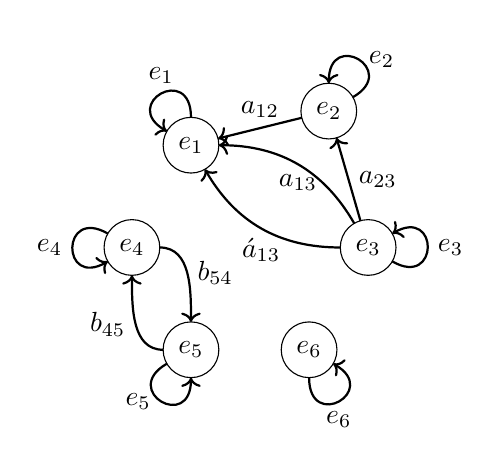
\begin{tikzpicture}
      \node[draw,  circle, outer sep=0pt] (a) at (0:1.5) {$e_3$};
      \node[draw,  circle, outer sep=0pt] (b) at (60:2) {$e_2$};
      \node[draw,  circle, outer sep=0pt] (c) at (120:1.5) {$e_1$};
      \node[draw,  circle, outer sep=0pt] (d) at (180:1.5) {$e_4$};
      \node[draw,  circle, outer sep=0pt] (e) at (240:1.5) {$e_5$};
      \node[draw,  circle, outer sep=0pt] (f) at (300:1.5) {$e_6$};
  
      \draw (a) edge[thick,->,out=-30,in=30, looseness=5, "$e_3$"{right}] (a);
      \draw (b) edge[thick,->,out= 30,in=90, looseness=5, "$e_2$"{right}] (b);    
      \draw (c) edge[thick,->,out= 90,in=150, looseness=5, "$e_1$"{above}] (c);    
      \draw (d) edge[thick,->,out=150,in=210, looseness=5, "$e_4$"{left}] (d);    
      \draw (e) edge[thick,->,out=210,in=270, looseness=5, "$e_5$"{left}] (e);    
      \draw (f) edge[thick,->,out=270,in=330, looseness=5, "$e_6$"{below}] (f); 
  
      \draw (a) edge[thick,->, "$a_{23}$"{right}] (b);
      \draw (b) edge[thick,->, "$a_{12}$"{above}] (c);
      \draw (a) edge[thick,->, bend right, "$a_{13}$"{below}] (c);
      \draw (a) edge[thick,->, bend left, "$\acute{a}_{13}$"{below}] (c);

      \draw (d) edge[thick,->,out=0,in=90, looseness=1, "$b_{54}$"{right}] (e);    
      \draw (e) edge[thick,->,out=180,in=-90, looseness=1, "$b_{45}$"{left}] (d);    

    \end{tikzpicture}
    \caption{Cayley graph}
    \label{fig:dots-arrows}
  \end{subfigure}
  \begin{subfigure}[b]{0.45\textwidth}
    \centering
    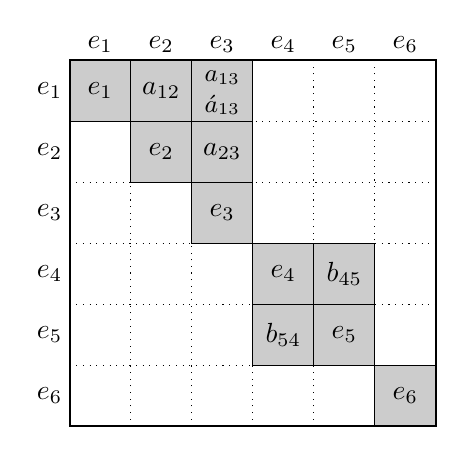
\begin{tikzpicture}[scale=1.25]
      \pgfmathsetmacro{\s}{0.62}
      \foreach \t in {0,...,5} {
        \draw[dotted] (0,\s*\t) -- ++(6*\s,0);
        \draw[dotted] (\s*\t,0) -- ++(0,6*\s);
        \draw[fill=black!20] (\s*\t,5*\s-\s*\t) rectangle node{$e_{\the\numexpr \t + 1\relax}$} ++(\s,\s);
      };
      \draw[thick] (0,0)  rectangle (6*\s,6*\s);      
      \draw[fill=black!20] (2*\s,4*\s) rectangle node{$a_{23}$} ++(\s,\s);
      \draw[fill=black!20] (1*\s,5*\s) rectangle node{$a_{12}$} ++(\s,\s);
      \draw[fill=black!20] (2*\s,5*\s) rectangle node{{\small $\begin{array}{c}a_{13} \\ \acute{a}_{13}\end{array}$}} ++(\s,\s);
      \draw[fill=black!20] (4*\s,2*\s) rectangle node{$b_{45}$} ++(\s,\s);
      \draw[fill=black!20] (3*\s,1*\s) rectangle node{$b_{54}$} ++(\s,\s);
      \node at (0.5*\s, 6.25*\s) {$e_1$};
      \node at (1.5*\s, 6.25*\s) {$e_2$};
      \node at (2.5*\s, 6.25*\s) {$e_3$};
      \node at (3.5*\s, 6.25*\s) {$e_4$};
      \node at (4.5*\s, 6.25*\s) {$e_5$};
      \node at (5.5*\s, 6.25*\s) {$e_6$};
      \node at (-0.33*\s, 5.5*\s) {$e_1$};
      \node at (-0.33*\s, 4.5*\s) {$e_2$};
      \node at (-0.33*\s, 3.5*\s) {$e_3$};
      \node at (-0.33*\s, 2.5*\s) {$e_4$};
      \node at (-0.33*\s, 1.5*\s) {$e_5$};
      \node at (-0.33*\s, 0.5*\s) {$e_6$};
    \end{tikzpicture}
    \caption{Peirce decomposition}
    \label{fig:Peirce}
  \end{subfigure}
  \caption{Visualizing the abstract category $\acat{A}$ in Example~\ref{ex:abscat}}
  \label{fig:abscat-prod}
\end{figure}


\subsection{Peirce decomposition of abstract categories}
\label{sec:Peirce}

Treating categories as algebraic structures allows us to frame aspects of
category theory in algebraic terms.  
Our goal is an elementary representation theory of categories. In
particular, we seek matrix-like structures---known as Peirce
decompositions in ring theory---for abstract categories.

One can recover from an abstract category $\acat{A}$ notions of objects and
morphisms by considering the identities $\one_{\cat{A}}$. Using the laws in
Definition~\ref{def:abs-cat},
\[
 (\forall e\tin \one_{\cat{A}})\;\;(\forall f\tin \one_{\cat{A}}) \;\;\;
    ef = 
    \begin{cases}
      e  & \text{ if } f = e, \\ 
      \bot & \text{ otherwise}. 
    \end{cases}
\]
In algebraic terms, the subtype $\one_{\cat{A}}$ is a type of pairwise 
orthogonal idempotents. For subtypes $X$ and $Y$ of $\acat{A}$, define
\[ 
 XY=\{xy\mid x\tin X, y\tin Y,\ \src{x}=\tgt{y}\}. 
\]

\begin{fact}\label{fact:capsule}
  If $a\tin\acat{A}$, then $\one_{\cat{A}} \{a\}=\{a\}=\{a\} \one_{\cat{A}}$;
  we write simply $\one_{\cat{A}} a=a=a\one_{\cat{A}}$.
\end{fact}

\noindent Given $e,f\tin\one_{\cat{A}}$, we define three subtypes:
\begin{align*}
  & (\text{left slice}) & e\acat{A} & = \{a\tin \acat{A} \mid e=\tgt{a}\}; \\
  & (\text{right slice}) & \acat{A}f & = \{ a\tin \acat{A} \mid \src{a}=f\};
  \\
  & (\text{hom-set}) & e\acat{A}f & = \{ a\tin \acat{A} \mid  e=\tgt{a},\ \src{a}=f\}.
\end{align*}
These subtypes appear in Figure~\ref{fig:peirce} in the left, middle, and right
images, respectively. If $\src{e}=\tgt{a}$ for $a:\acat{A}$, then
$ea=(\src{e})a=(\tgt{a})a=a$.


\begin{figure}[!htbp]
  \centering
  \begin{tikzpicture}
    \pgfmathsetmacro{\mylen}{3}
    \node (leftcoset) at (-4,0) {\begin{tikzpicture}
      \foreach \t in {0,...,6} {
        \draw[dotted] (0,0.5*\t) -- ++(\mylen,0);
        \draw[dotted] (0.5*\t,0) -- ++(0,\mylen);
      };
      \draw[thick] (0,0)  rectangle (\mylen,\mylen);      
      \draw[fill=black!20] (0,0.5) rectangle (\mylen,1.0);
      \node[scale=0.75] (A) at (1.25,0.75) {$e\acat{A}$};
      \node at (-0.25, 0.75) {$e$};
      \node at (1.25, 3.25) {$\phantom{f}$};
    \end{tikzpicture}};

    \node (rightcoset) at (0,0) {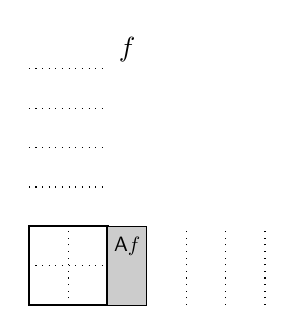
\begin{tikzpicture}
      \foreach \t in {0,...,6} {
        \draw[dotted] (0,0.5*\t) -- ++(\mylen,0);
        \draw[dotted] (0.5*\t,0) -- ++(0,\mylen);
      };
      \draw[thick] (0,0)  rectangle (\mylen,\mylen);      
      \draw[fill=black!20] (1.0,0) rectangle (1.5,\mylen);
      \node[scale=0.75] (A) at (1.25,0.75) {$\acat{A}f$};
      \node at (1.25, 3.25) {$f$};
    \end{tikzpicture}};

    \node (innercoset) at (3.75,0) {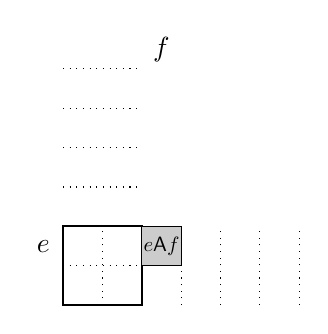
\begin{tikzpicture}
      \foreach \t in {0,...,6} {
        \draw[dotted] (0,0.5*\t) -- ++(\mylen,0);
        \draw[dotted] (0.5*\t,0) -- ++(0,\mylen);
      };
      \draw[thick] (0,0)  rectangle (\mylen,\mylen);      
      \draw[fill=black!20] (1.0,0.5) rectangle (1.5,1.0);
      \node[scale=0.75] (A) at (1.25,0.75) {$e\acat{A}f$};
      \node at (-0.25, 0.75) {$e$};
      \node at (1.25, 3.25) {$f$};
    \end{tikzpicture}};
  \end{tikzpicture}
  \caption{Visualizing the Peirce decomposition of $\acat{A}$}
  \label{fig:peirce}
\end{figure}


If $a\tin \acat{A}$, then $a\tin \acat{A} (\src{a})$, and so on, from which we
deduce the following. 

\begin{prop}
  \label{prop:Peirce-decomposition}
  If $\acat{A}$ is an abstract category, then $a\mapsto (\tgt{a})a$, 
  $a\mapsto a(\src{a})$, and $a\mapsto (\tgt{a})a(\src{a})$ induce  
  invertible functions $($denoted by ``$\leftrightarrow$"$)$ of the following types:
    \begin{align*}
      \acat{A} &\longleftrightarrow \bigsqcup_{e\tin \one_{\cat{A}}} e\acat{A}, 
      &
      \acat{A} &\longleftrightarrow \bigsqcup_{f\tin \one_{\cat{A}}}\acat{A}f 
      &
      \acat{A} &\longleftrightarrow \bigsqcup_{e\tin \one_{\cat{A}}} \bigsqcup_{f\tin \one_{\cat{A}}} e\acat{A}f.
    \end{align*}
\end{prop}

Proposition~\ref{prop:Peirce-decomposition}, which we use to prove Theorem~\ref{thm:extension},
allows us to draw upon intuition from matrix algebras.  
The morphisms of a category appear in its multiplication table, as in 
Table~\ref{tab:comp-grammer-table}. Products of morphisms and slices are defined, as with
matrix products, only when the inner indices agree. In this model, $\one_{\cat{A}}$ can be
visualized as the identity matrix, where the entries on the diagonal are the
individual identities $e\tin \one_{\cat{A}}$. In Figure~\ref{fig:Peirce}, 
that product is
represented in a matrix-like form respecting the conditions of the Peirce
decomposition.

\begin{rem}
  \label{rem:bi-inter} 
  While there are differences between the types for categories and 
abstract categories, every theorem stated in one
  setting translates to a corresponding theorem in the other.  More
  precisely, the translation is a model-theoretic \emph{definable
  interpretation}~\cite{Marker:models}*{\S1.4}: there is a prescribed
  formula that translates every theorem and its proof between the two theories.
  Example~\ref{ex:abscat} shows how the model of categories with both objects and
  morphisms may be interpreted as definable types in the
  theory of categories with only morphisms (abstract categories). Conversely, if
  $\acat{A}$ is an abstract category, then we obtain a category
  $\cat{C}$ with object type $\cat{C}_0\defeq \one_{\acat{A}}$ as follows. For objects 
  $e,f\tin \cat{C}_0$, we define 
  \[ 
    \cat{C}_1(e,f)  \defeq  f \cat{A} e,
  \]
  where the identity morphisms of $\acat{C}$ are $e:\cat{C}_1(e,e)$.
  To compose morphisms $fae : \cat{C}_1(e,f)$ with $gbf:\cat{C}_1(f,g)$ for objects $e,f,g:\cat{C}_0$, we define 
  \[
    (gbf)(fae) \defeq gbae : \cat{C}_1(e, g).
  \]  
  Hence, we no longer distinguish between categories and
  abstract categories. 
\end{rem}

\subsection{Eastern algebras as categories}
Example \ref{ex:cats-Eastern} shows that a category is an eastern algebra. 
We now show that a variety of eastern algebras forms a category.

\begin{defn}\label{def:mor-Omega}
  Fix a signature $\Omega$. Let $E_1,E_2:\East_\Omega$, where $E_1 = \langle A, \Phi,
  \omega \mapsto \langle \omega_A , p\rangle\rangle$ and $E_2 = \langle B, \Gamma,
  \omega \mapsto \langle \omega_B , q \rangle\rangle$. A \emph{morphism} from
  $E_1$ to $E_2$ is a partial-function $f:A\to B^?$ such that for every 
  $\omega:\Omega$ and every $a_1,\ldots, a_{|\omega|}:A$,
  \begin{align*} 
    f(\omega_{\type{A}}(a_1,\ldots,a_{|\omega|}))
      \venturi 
    \omega_{\type{B}}(f(a_1),\ldots,f(a_{|\omega|})).
  \end{align*}
  The type of morphisms from $E_1$ to $E_2$ is 
  \begin{align*}
    \ftor_{\Omega}(E_1, E_2) &\defeq \bigsqcup_{f : A \to B^?} ~\prod_{\omega : \Omega} ~\prod_{a: A^{|\omega|}}\left(f(\omega_{\type{A}}(a_1,\ldots,a_{|\omega|}))
    \venturi 
  \omega_{\type{B}}(f(a_1),\ldots,f(a_{|\omega|}))\right) .
  \end{align*}
\end{defn}

The object type $\East_{\Omega}$ and the morphism type $\ftor_{\Omega}$ form the
category of $\Omega$-eastern algebras. In particular, the
$\Omega$-morphisms of $\East_\Omega$, namely the type 
\[ 
  \ftor_{\Omega} \defeq \bigsqcup_{E_1 : \East_\Omega}~\bigsqcup_{E_2 : \East_\Omega} \ftor_{\Omega}(E_1,E_2),
\] 
can be viewed as an abstract category (see Proposition~\ref{prop:morph_laws}). Therefore,
$\ftor_{\Omega}$ forms an eastern algebra with the composition signature.

We call a subcategory $\acat{E}$ of eastern algebras an \emph{eastern variety}
(with respect to signature $\Omega$ and laws $\mathcal{L}$) if it is full and
its objects are those eastern $\Omega$-algebras satisfying the laws
$\mathcal{L}$. We reserve $\acat{E}$ to denote an eastern variety.

\begin{rem}
  \label{rem:[paradox]} Regarding categories as eastern algebras could lead to a
  paradox of Russell type.
  The paradox is avoided either by limiting $\Pi$-types to forbid some
  quantifications~\cite{Tucker} or by creating an increasing tower of universe
  types and pushing the larger categories into the next
  universe~\cite{HoTT}*{\S9.9}.  Both resolutions allow us to define
  categories and eastern algebras computationally.
\end{rem}

Under the correspondence of Remark~\ref{rem:bi-inter}, morphisms between
abstract categories are precisely functors between categories. This translation
serves two of our goals.  The first is an elementary representation theory for
categories: by regarding categories as ``monoids with partial-operators", we
mimic monoid actions.  The second is to treat a category as a single data type
with operations defined on it.  This is considerably easier to implement as a
computer program. Indeed, both {\sf GAP} \cite{GAP4} and {\sc Magma}
\cite{magma} are designed for such algebras. There are benefits to the usual
description of categories, but the translation to abstract categories is
essential for our approach to  computing with and within categories.

Next, we prove a generalization of Noether's Isomorphism Theorem.
\enlargethispage{0.3cm}

\begin{thm}
\label{thm:Noether}
  Let $\varphi : E_1 \to E_2$ be a morphism between eastern algebras. There
  exist eastern algebras $\mathrm{Coim}(\varphi)$ and $\mathrm{Im}(\varphi)$, an
  epimorphism $\mathrm{coim}(\varphi) : E_1 \twoheadrightarrow
  \mathrm{Coim}(\varphi)$, a monomorphism $\mathrm{im}(\varphi) :
  \mathrm{Im}(\varphi) \hookrightarrow E_2$, and an isomorphism $\psi :
  \mathrm{Coim}(\varphi) \to \mathrm{Im}(\varphi)$ such that the  
  following diagram commutes.
  \begin{center}
    \begin{tikzcd}
      E_1 \arrow[r, "\varphi"] \arrow[d, twoheadrightarrow, "\mathrm{coim}(\varphi)", swap] & E_2 \\
      \mathrm{Coim}(\varphi) \arrow[r, "\psi"] & \mathrm{Im}(\varphi) \arrow[u, hook, "\mathrm{im}(\varphi)", swap]
    \end{tikzcd}
  \end{center}
\end{thm}

\begin{proof}
  Let $\Omega$ be a signature, and let $A$ be an $\Omega$-eastern algebra. If
  every operation in $A$ is total, then we apply
Noether's Isomorphism Theorem~\cite{Cohn}*{Theorem~II.3.7}. It is clear that the existence of the stated algebras and morphisms is constructive.

  Otherwise, at least one operation is a partial-function. We define a new
  eastern algebra where all operations are total. Let $\NaN$ be a formal symbol,
  disjoint from $\Omega$. Define a new type $E \defeq A \sqcup \{\NaN\}$ with
  inclusion function $\iota_A : A \hookrightarrow E$. By abuse of notation, we also apply $\iota_A$ to tuples over $A$. Define a new signature
  $\Sigma$, obtained from $\Omega$ by including $\NaN$ as a constant. We use
  trivial rails for every operator, and define $\omega_E : E^{|\omega|} \to E$ via 
  \[ 
    e\mapsto \begin{cases}
      \iota_A(\omega_A(a)) & \text{if $e=\iota_A(a)$ for some $a: A^{|\omega|}$ with $\omega_A(a):A$,} \\
      \NaN  & \text{otherwise}.
    \end{cases}
  \] 
  Now every operation in $E$ is total, so the Isomorphism Theorem applies.
  Since every homomorphism of $\Sigma$-eastern algebras fixes constants, the
  statement follows. 
\end{proof}

The monomorphism $\mathrm{im}(\varphi)$ from Theorem~\ref{thm:Noether} is the
\emph{image} of $\varphi$, and the epimorphism $\mathrm{coim}(\varphi)$ is the
\emph{coimage} of $\varphi$. 
Theorem~\ref{thm:Noether} asserts, in particular, that categories of eastern 
algebras have images and coimages.
These maps possess universal properties~\cite{Riehl}*{\S E.5}.

\subsection{Subobjects and images}
\label{sec:subobjects-images}

We close with a list of facts about eastern varieties, which we use heavily in Section~\ref{sec:induced}. We first define a pre-order that enables abbreviation of compositions of multiple morphisms. To motivate this, assume $\varphi : E_1\to E_2$ is a morphism of eastern
algebras. Theorem~\ref{thm:Noether} states there exists $\theta : E_1 \to
\mathrm{Im}(\varphi)$ such that $\varphi = \mathrm{im}(\varphi) \theta$. We
denote this by $\varphi\ll \mathrm{im}(\varphi)$ and make the following more
general definition. For morphisms $a,b\tin \acat{E}$, 
\begin{align}
  \label{eq:pre-order}
  a &\ll b \iff  \left[(\exists c:\acat{E})\;\; 
  a=bc\right], \\
  \label{eq:dual-ll}
  a &\gg b \iff  \left[(\exists d:\acat{E})\;\; 
  a=db\right].
\end{align}
Two monomorphisms $a,b:\acat{E}$ are \emph{equivalent} if $a\ll b$ and
$b\ll a$. Similarly, epimorphisms $c,d:\acat{E}$ are \emph{equivalent} if $c\gg
d$ and $d\gg c$.

\begin{lem}\label{lem:im}
  Let $\acat{E}$ be an eastern variety. 
For morphisms $a,b\tin \acat{E}$, if 
  $\src{a}=\tgt{b}$, then $a\,\mathrm{im}(b) \ll \mathrm{im}(ab)$.
\end{lem}

\begin{proof}
  By Theorem~\ref{thm:Noether}, there exist isomorphisms $\psi_b, \psi_{ab} : \acat{E}$
  such that 
  \begin{align*}
    b &= \mathrm{im}(b)\psi_b\mathrm{coim}(b), & ab &= \mathrm{im}(ab)\psi_{ab}\mathrm{coim}(ab) .
  \end{align*}
  By the universal property of coimages, there exists a unique morphism
  $\pi:\acat{E}$ such that $\mathrm{coim}(ab) = \pi\,\mathrm{coim}(b)$.
  Therefore, 
  \begin{align*}
    a\,\mathrm{im}(b)\psi_b\mathrm{coim}(b) = ab = \mathrm{im}(ab) \psi_{ab} \mathrm{coim}(ab) = \mathrm{im}(ab) \psi_{ab} \pi\, \mathrm{coim}(b).
  \end{align*}
  Since $\mathrm{coim}(b)$ is an epimorphism, $a\,\mathrm{im}(b) =
  \mathrm{im}(ab) \psi_{ab} \pi \psi_b^{-1} \ll \mathrm{im}(ab)$.
\end{proof}

\begin{lem}\label{lem:im-monic}
  Let $\acat{E}$ be an eastern variety. For morphisms $a,b\tin \acat{E}$, if
  $\src{a}=\tgt{b}$, then 
  $\mathrm{im}(ab)\ll \mathrm{im}(a)$. If $a$ is also monic, then 
  $\mathrm{im}(ab) \ll a\,\mathrm{im}(b)$.
\end{lem}

\begin{proof}
  The first claim follows from the universal property of images, so we assume $a$ is monic.
  By Theorem~\ref{thm:Noether}, there exists an isomorphism $\psi_b : \acat{E}$ such
  that 
  \begin{align*}
    b &= \mathrm{im}(b)\psi_b\mathrm{coim}(b) .
  \end{align*}
  Since $a\,\mathrm{im}(b)$ is monic and
  $ab=(a\,\mathrm{im}(b))(\psi_b\mathrm{coim}(b))$, by the universal property of
  images, there exists a morphism $\iota : \acat{E}$ such that $\mathrm{im}(ab)
  = a\,\mathrm{im}(b)\iota\ll a\,\mathrm{im}(b)$.
\end{proof}

Eastern varieties have a \emph{coproduct}~\cite{Riehl}*{p.~81} given by
the \emph{free product}~\cite{Riehl}*{p.~183}.  
An example concerning groups is given in \cite{Riehl}*{Corollary 4.5.7}. 
We list some facts concerning coproducts in eastern varieties.

\begin{fact}
  \label{fact:coprod}
  Let $I$ be a type. In an eastern variety $\acat{E}$,
  the following hold for all $e:\one_{\acat{E}}$ and $a:I\to e\acat{E}$.
  \begin{ithm}
    \item\label{factpart:coprods} There exists a coproduct morphism
    $\coprod_{i:I}a_i$ and morphisms $\iota:I\to
    \big(\coprod_{i:I}a_i\big)\acat{E}$ satisfying
    $\big(\coprod_{i:I}a_i\big)\iota_j=a_j$ for each $j:I$.

    \item\label{factpart:empty-coprod} If $I$ is uninhabited, then
    $f=\src{\left(\coprod_{i:I}a_i\right)}$ is the identity on the free algebra
    on the empty set. In particular, $\coprod_{i:I}a_i$ is the unique morphism
    inhabiting $e\acat{E}f$.

    \item\label{factpart:factor-out} If $b\tin \acat{E}$ such that
    $\src{b}=\tgt{a_i}$ for all $i:I$, then $\coprod_{i:I}(b a_i)=b
    \coprod_{i:I}a_i$. 

    \item\label{factpart:ignore-inside} If $b:I\to \acat{E}$ with
    $\src{a_i}=\tgt{b_i}$ for all $i:I$, then $\coprod_{i:I} (a_i b_i)\ll
    \coprod_{i: I}a_i$.

    \item\label{factpart:smaller-coprod} If $J\subset I$, then $\coprod_{j:J}a_j
    \ll \coprod_{i:I}a_i$.
  \end{ithm}
\end{fact}

Finally, if $a$ is monomorphism satisfying 
$\tgt{a}=e$, for some identity $e$, then $\src{a}$ can be regarded as 
a subobject of the object associated to $e$. 
Given a collection $\{a_i\mid i:I\}$ of such monomorphisms,
consider the smallest subobject 
containing all set-wise images of the $\src{a_i}$.  
The coproduct allows us to effectively ``glue" together 
all of the monomorphisms, but the result is not a monomorphism.  
To obtain a monomorphism, we take the image of the coproduct, 
namely
\begin{align}\label{eq:coprod_im_comment}
  \text{im}\left(
    \coprod_{i:I} a_i
  \right).
\end{align}

\section{Category actions, capsules, and counits}
\label{sec:actions}

Theorem~\ref{thm:char-repn} asserts that characteristic subgroups arise from categories
acting on other categories. 

\subsection{Category actions}
\label{sec:cat-acts-biacts}
Our formulation of category actions generalizes the familiar notion for groups
and also actions of monoids and groupoids ~\cite{MonoidsAC}*{\S I.4}. The
technical aspects of the definition concern the additional guards, denoted
$\lhd$, needed to express where products are defined. Their use is similar to
the guards $\blacktriangleleft$ used for abstract categories (see
Definition~\ref{def:abs-cat}). 

\newcommand{\actX}{\aX} 
\newcommand{\actY}{\aY}
\newcommand{\biactionpair}{biaction pair}
\newcommand{\myopp}{\lhd X}

\begin{defn}
\label{def:cat-act}
  Let $\cA$ be an abstract category with guards denoted by $\src{(-)}$ and
  $\tgt{(-)}$. Let $X$ be a type. A \emph{$($left$)$ category action} of
  $\cA$ on $X$ consists of a type $\myopp$, functions 
  $(-)\lhd:\cA\to \myopp$ and $\lhd(-):X\to \myopp$, and a 
  partial-function $\cdot: \cA\times X\to X^?$ that satisfies the following 
  rules: \\[1ex]
  \hspace*{0.5cm}\begin{tabular}{llll}
    (1) & ($\forall a:\cA$) & ($\forall x:X$) &  $\left[(a\lhd=\lhd x)\iff ((\exists y:X)\; a\cdot x=y)\right]$;\\[0.5ex]
    (2) & ($\forall a:\cA)$  & ($\forall x:X$) & $\left[(\src{a})\lhd=a\lhd\text{ and } ((\src{a})\cdot x) \venturi x\right]$; and\\[0.5ex]
    (3) & ($\forall a,b:\cA$) & ($\forall x:X$) &  $((ab)\cdot x) \venturi (a\cdot (b\cdot x))$.
  \end{tabular}

\vspace*{1ex}
  
  Given a left action of $\cA$ on a type $Y$, a partial-function $\fM:X\to Y^?$
  is an \emph{$\cA$-morphism} if $\fM(a\cdot x) = a \cdot \fM(x)$ whenever
  $a:\cA$ and $x:X$ with $a\lhd=\lhd x$.
\end{defn}

Right category actions are similarly defined. 
We unpack the symbolic expressions in Definition~\ref{def:cat-act}. Condition
(1) states that the functions $(-)\lhd$ and $\lhd (-)$ serve as guards for the
partial-function $\cdot : \cA\times X\to X^?$: namely, (1)
characterizes precisely when $\cdot$ is defined. The first part of Condition (2)
asserts that $(-)\lhd$ respects the $\src{(-)}$ identity of $\acat{A}$; the
second part states that identity morphisms of $\acat{A}$ act as identities.
Condition (3) is the familiar group action axiom in the setting of
partial-functions.

For subtypes $S\subset \acat{A}$ and $Y\subset X$, we write
\begin{align*}
  S\cdot Y & = \{ s\cdot y\mid s\tin S,\; y\tin Y,\; s\lhd =\lhd y\}.
\end{align*}
From Definition~\ref{def:cat-act}, an $\acat{A}$-morphism $\fM:X\to Y^?$ is
always defined on $\acat{A}\cdot X$; 
hence, we do not need guards for $\acat{A}$-morphisms. 

\begin{defn}
  The category action of $\acat{A}$ on $X$ is \emph{full} if $e\cdot x \mapsto
  \lhd(e\cdot x)$ defines a bijection from $\one_{\acat{A}}\cdot X$ to
  $\cA\lhd = \{a \lhd \mid a :\acat{A}\}$.
\end{defn}
\noindent
Note that the category action of $\cA$ on $X$ is full if and only if for every 
$a:\cA$ there exists an $x:X$ such that $a\lhd =\lhd x$. 

Since we identify categories and abstract categories (Remark~\ref{rem:bi-inter}), we
say that a category $\cC$ acts on a type $X$ if its morphisms
$\cC_1$ act on $X$.

\begin{ex}
  Let $\cat{C}$ be a category with object type $\cat{C}_0$ and morphism type
  $\cat{C}_1$. Set $X = \myopp = \cat{C}_0$. Define $(-)\lhd : \cat{C}_1 \to
  \cat{C}_0$ via $f\lhd \defeq \Dom f$ and define $\lhd (-) : \cat{C}_0 \to
  \cat{C}_0$ via $\lhd \,U \defeq U$. Let $\cdot : \cat{C}_1 \times \cat{C}_0\to
  \cat{C}_0^?$ be the partial-function defined by 
  \begin{align*}
    f\cdot U \defeq \begin{cases}
      \Codom f & \text{if } f\lhd = \lhd \,U, \\
      \bot & \text{otherwise}.
    \end{cases}
  \end{align*}
  This defines a full left action of $\cat{C}$ on $\acat{C}_0$. A full right
  action is defined similarly.~\exqed
\end{ex}

\begin{rem}
  Let $\acat{C}$ be a category and let $X=\acat{C}_1$. The
  definition of category action 
  in~\cite{FS}*{1.271--1.274} is similar to ours, but it requires
  $\myopp=\one_{\acat{C}}=\{\src{f} \mid f\tin\acat{C}_1\}$ and $\lhd
  x=\tgt{x}$ and $f\lhd =\src{f}$ for every $x\tin X$ and $f\tin
  \acat{C}_1$. Thus, for $f,g\tin \acat{C}_1$ and $x\tin X$, both $f\cdot
  x$ and $g\cdot x$ are defined only when $\src{f}=\lhd x=\src{g}$; this is too
  restrictive for our purposes.
\end{rem}

\subsection{Capsules}
As identified in Section~\ref{sec:local-to-global}, we focus on the action of
one category $\cat{A}$ on another category $\cat{X}$; we call these ``category
modules'' \emph{capsules}. Note the change in notation from $X$ to $\cat{X}$ 
to emphasize this setting.
In this case, $\cat{X}$ already has a candidate type
for $\lhd \cat{X}$, namely $\tgt{\cat{X}}=\one_{\cat{X}}$. Furthermore, because
a category has its own operation of composition, the action by $\cat{A}$
respects composition.  For example, given a group homomorphism
$\varphi:G\to H$, we get an action $g\cdot h\defeq \varphi(g)h$ that satisfies
$g\cdot (hh')=(g\cdot h)h'$. 

\begin{defn}\label{def:vanilla} 
  A category $\cat{X}$ is a \emph{left $\acat{A}$-capsule} if there is a full left
  $\acat{A}$-action on $\acat{X}$ with $\lhd \acat{X} = \one_{\acat{X}}$ such
  that the following hold:\\[1ex]
  \hspace*{0.5cm}\begin{tabular}{llll}
    (a) & $(\forall x:\acat{X})$& $(\lhd x = \tgt{x})$;\\
    (b) & $(\forall a:\acat{A})$ & $(\forall x,y: \acat{X})$ & $a\cdot (xy)\asymp
    (a\cdot x)y$.
  \end{tabular}
\end{defn}
A \emph{right $\acat{A}$-capsule} is similarly defined.  
We present our results below 
for left $\acat{A}$-capsules, but they can be formulated for both.

Much of our intuition on actions draws on familiar themes in representation
theory. A reader may be assisted by translating ``$\cA$-capsule'' to
``$A$-module'' and considering the matching statement for modules.  We write
${_{\cA} {\acat{X}}}$ to indicate the presence of a left $\acat{A}$-capsule action
on $\aX$.

From now on, if a category $\acat{A}$ acts on
itself, then we assume it is by the (left) \emph{regular action}, 
where $\cdot : \acat{A}\times \acat{A} \to \acat{A}^?$ is given 
by composition in $\acat{A}$. Moreover, a
category action on another category is implicitly understood to be on the
morphisms. We now show that capsules arise from morphisms between
categories. 

\begin{prop}
  \label{prop:functors-are}
    A category $\cX$ is a left $\cA$-capsule 
    of a category $\cA$ if, and only if, there is a morphism $\fF:\cA\to \cX$ such 
    that $a\cdot x=\fF(a)x$. Furthermore, the morphism $\fF$ is unique.
\end{prop}

The following lemma proves one direction of Proposition~\ref{prop:functors-are}.
  
\begin{lem}
  \label{lem:induced-act}
    Every morphism $\fF:\cA\to\cX$ of categories makes $\cX$ a left 
$\acat{A}$-capsule,
    where for each $a:\cA$ and $x:\cX$, the guard is defined by
    $\text{$a\lhd\defeq\src{\fF(a)}$}$ and the action is defined by $a\cdot
    x\defeq \fF(a)x$. 
\end{lem}

\begin{proof}
Condition (1) of Definition~\ref{def:cat-act} is satisfied by the defined action.

  For the first part of Condition (2), let $a\tin\acat{A}$. Since $\func{F}$ is
  a morphism and $\src{(-)}$ is everywhere defined,
  $\func{F}(\src{a})=\src{\func{F}(a)}$. Hence, by
  Lemma~\ref{lem:idempotent-guards}\ref{lempart:idem}, 
  \begin{align*}
    (\src{a})\lhd & = \src{\func{F}(\src{a})} = \src{(\src{\func{F}(a)})} = \src{\func{F}(a)} = a\!\lhd.
  \end{align*}
  For the second part of Condition (2), let $a\tin\acat{A}$ and $x\tin\acat{X}$
  with $a\lhd=\lhd x$, so $\src{\func{F}(a)} =\tgt{x}$ by definition. Thus,
  $$(\src{a}) \cdot x = \func{F}(\src{a})x = (\src{\func{F}(a)})x = (\tgt{x}) x =
  x,$$ so $(\src{a})\cdot x\venturi x$ for every $a:\acat{A}$ and $x:\acat{X}$. 

  For Condition (3), let $a,b\tin\acat{A}$ and $x\tin\acat{X}$ with $\src{a} =
  \tgt{b}$ and $(ab)\lhd=\lhd x$, so $(ab)\cdot x$ is defined and
  $\src{(ab)}=\src{b}$. We need to show that $(ab)\cdot x=a\cdot (b\cdot x)$.
  Since $\func{F}$ is a morphism, 
  $$
    (ab)\lhd=\src{(\func{F}(ab))}=\func{F}(\src{(ab)})=\func{F}(\src{b})=\src{\func{F}(b)}=b\lhd.
  $$ 
  Hence, $(ab)\lhd=\lhd x$ implies $b\lhd =\lhd x$. Thus, $\func{F}(b)x$ is
  defined. Also,  $\src{a} = \tgt{b}$ implies $\src{\func{F}(a)} =
  \tgt{(\func{F}(b))}$, so
  \[
    a \lhd = \src{\func{F}(a)} = \tgt{(\func{F}(b))} =\tgt{(\func{F}(b)x)}=\tgt{(b\cdot x)}=\lhd (b\cdot x).
  \]
  It follows that $a\cdot (b\cdot x)$ is defined. Since $\func{F}$ is a
  morphism, 
  $$
    a\cdot (b\cdot x) = \func{F}(a)(\func{F}(b)x) = \func{F}(ab)x = (ab)\cdot x,
  $$ 
  and therefore $(ab)\cdot x \venturi a\cdot (b\cdot x)$ for every
  $a,b\tin\acat{A}$ and $x\tin\acat{X}$.

  To see that the action is full, consider  $a\tin \acat{A}$ and define
  $x=\src{\func{F}(a)}$. By the laws of an abstract category,  
  $a \lhd = \src{\func{F}(a)} = \tgt{({\src{\func{F}(a)}})} = \tgt{x} = \lhd x$.
  Finally, $(a\cdot x)y=\fF(a)xy\asymp a\cdot (xy)$, so $\cX$ is a left
  $\cat{A}$-capsule.
\end{proof}

Our proof of the reverse direction of  Proposition~\ref{prop:functors-are} uses
the following result.\enlargethispage{0.3cm}

\begin{lem}
  \label{lem:unique-identity}
  Let $\acat{X}$ be a left $\acat{A}$-capsule. For every $a\tin \cA$, there is a unique
  $e:\one_{\aX}$ such that $a\cdot e$ is the unique term of type
  $a\cdot\one_{\aX}$.
\end{lem}

\begin{proof}
  Since the action is full, for each $a\tin \acat{A}$ there exists
  $x\tin\aX$ such that $a\lhd = \lhd x$, so $a\cdot x$ is defined.
  Since $\acat{X}$ is a left $\acat{A}$-capsule, $a\lhd = \lhd x = \tgt{x}$, so
  \[
    \lhd(\tgt{x})=\tgt{(\tgt{x})}=\tgt{x}.
  \]
  Hence, $a\cdot (\tgt{x})$ is defined and has type $a\cdot \one_{\aX}$.
  Suppose $e,f\tin\one_{\acat{X}}$ and $a\lhd = \lhd e = \lhd f$, so that
  $a\cdot e, a\cdot f \tin a\cdot \one_{\aX}$.  Furthermore, 
  \[
    e = \tgt{e} = \lhd e = \lhd f = \tgt{f} = f.
  \] 
  Thus, $a\cdot e = a\cdot f$, and there is exactly one term with type $a\cdot
  \one_{\aX}$.
\end{proof}

Under the assumptions of Lemma~\ref{lem:unique-identity}, we simplify notation and
identify $a\cdot \one_{\acat{X}}$ with its unique term. 

\begin{proof}[Proof of Proposition~$\ref{prop:functors-are}$]
  By Lemma~\ref{lem:induced-act}, it remains to prove the forward direction and uniqueness. 
  Suppose that $\cX$ is a left $\cA$-capsule.
  By Lemma~\ref{lem:unique-identity}, for each $a:\cA$ there is a unique
  $\fF(\src{a}):\one_{\cX}$ such that $(\src{a})\cdot \fF(\src{a})$ is defined.
  Since $\cX$ is a left $\cA$-capsule and $\fF(\src{a})$ is an identity,
  \[
    (\src{a})\lhd=a\lhd=\lhd\fF(\src{a})=\tgt\fF(\src{a})=\fF(\src{a}).
  \]
  Thus, $a\cdot \fF(\src{a})$ is also defined. Put $\fF(a)\defeq a\cdot
  \fF(\src{a})$. If $x:\cX$, then $a\cdot x$ is defined whenever 
  \[
    \tgt{x}=\lhd x=a\lhd=\fF(\src{a})=\src{\fF(\src{a})}.
  \]
  Hence, $\fF(\src{a})x$ is also defined in $\cX$. Because $\fF(\src{a})$ is an
  identity, $\fF(\src{a})x=x$.  Since $\acat{X}$ is a left $\acat{A}$-capsule, $a\cdot x=a\cdot
  (\fF(\src{a}) x)=(a\cdot \fF(\src{a}))x=\fF(a)x$. Hence, it remains to prove
  that $\fF:\cA\to \cX$ is a morphism of categories.

  For $a,b\tin \acat{A}$, by the action laws
  \begin{align*}
    \func{F}(ab) 
     & \asymp (ab)\cdot \fF(\src{(ab)})
      \asymp (ab)\cdot \fF(\src{b})
      \venturi a\cdot (b\cdot \fF(\src{b}))
     \asymp a\cdot \func{F}(b).
  \end{align*}
  Thus, $\func{F}(ab) \venturi a\cdot \func{F}(b)$. 
But $\cX$ is a left $\cA$-capsule, so Fact~\ref{fact:capsule} implies that
  \begin{align}\label{eqn:act-comp}
    a\cdot \func{F}(b) &\asymp a\cdot (\one_{\cX}\func{F}(b)) \asymp (a\cdot \one_{\cX}) \func{F}(b) \asymp \func{F}(a)\func{F}(b).
  \end{align}
  Hence, $\func{F}(ab) \venturi \func{F}(a)\func{F}(b)$. By Lemma~\ref{lem:idempotent-guards}\ref{lempart:guard-reduc} and \eqref{eqn:act-comp} for all $a:\cA$, 
  \[
    \src{\fF(a)}= \src{(a\cdot \fF(\src{a}))}=\src{(\fF(a) \fF(\src{a}))}=\src{\fF(\src{a})}=\fF(\src{a}).
  \]
  Similarly, $\func{F}(\tgt{a}) = \tgt{\func{F}(a)}$. Hence, $\fF$ is a
  morphism.

  Lastly, we prove uniqueness of  $\fF$. Suppose there exists $\func{G}:
  \cA\to \cX$ such that $a\cdot x = \func{G}(a)x$ for every $a:\cA$ and $x:\cX$
  whenever $a\lhd = \lhd x$. Since $a\lhd=\fF(\src{a})$, it follows that
  $\src{\fG(a)}=\fF(\src{a})$, so $\func{G}(a) = \func{G}(a)\fF(\src{a}) =
  a\cdot \fF(\src{a})  = \fF(a)$.
\end{proof}

If $\acat{B}$ is a subcategory of $\acat{A}$ with inclusion $\func{I} :
\acat{B}\to\acat{A}$, then the (left) \emph{regular action} of $\acat{B}$ on
$\acat{A}$ is defined to be the action given by $\func{I}$. In other words, the regular action
of $\acat{B}$ on $\acat{A}$ is given by $b\cdot a = \func{I}(b)a$ for
$a:\acat{A}$ and $b:\acat{B}$. By Lemma~\ref{lem:induced-act}, each regular
action defines a capsule.  With regular actions we sometimes omit the ``$\cdot$''.


\subsection{Category biactions and cyclic bicapsules}\label{sec:cat-biacts}

We now define the concepts appearing in Theorem~\ref{thm:char-repn}(3).

\begin{defn}\label{defn:bi-action}
  Let $\cA$ and $\cB$ be categories and let $X$ and $Y$ be types.
  \begin{ithm}
  \item An $(\cA,\cB)$-\emph{biaction} on $X$ is a left $\cA$-action on $X$
  and a right $\acat{B}$-action on $X$ such that $a\cdot (x\cdot b) \asymp
  (a\cdot x)\cdot b$ for every  $a\tin\cA$, $b\tin\cB$, and $x\tin X$. Hence,
  writing $a\cdot x\cdot b$ is unambiguous. If, in addition, $\aX$ is a left
  $\cA$-capsule and right $\cB$-capsule, then $\aX$ is an
  \emph{$(\cA,\cB)$-bicapsule}.

  \item Suppose there are $(\cA,\cB)$-biactions on $X$ and $Y$. An
  \emph{$(\cA,\cB)$-morphism} is a partial-function $\fM:X\to Y^?$ such that
  $\fM(a\cdot x\cdot b) = a\cdot \fM(x) \cdot b$, whenever
  $a:\cA$, $x:X$, $b:\cB$ with $a\lhd=\lhd x$ and $x\lhd=\lhd b$.
  \end{ithm}
\end{defn}

We sometimes write ${_{\cA}X_{\cB}}$ for an $(\cA,\cB)$-biaction on $X$ for
clarity.  Notice that an $(\cA,\cB)$-morphism $\fM:X\to Y^?$ must be defined on
$\cA\cdot X\cdot \cB$. As with capsule morphisms, we do not need to establish
guards. We abbreviate $(\cA,\cA)$-bicapsule to \emph{$\cA$-bicapsule},
$(\cA,\cA)$-morphism to \emph{$\cA$-bimorphism}, and $(\cA,\cA)$-biaction to
\emph{$\cA$-biaction}. Note that $\acat{A}$-bimorphisms are defined everywhere.
Just as ring homomorphisms are not always linear maps, morphisms of capsules
need not be morphisms of categories---morphisms of capsules do not in general
send identities to identities. 

Motivated by Proposition~\ref{prop:functors-are}, we show that bicapsules
provide a computationally useful perspective to record natural transformations
of functors. If $\func{F},\func{G}:\acat{A}\to\acat{B}$ are functors and $\mu:
\func{G}\Rightarrow \func{F}$ is a natural transformation, then, using
Remark~\ref{rem:bi-inter}, the natural transformation property written with guards is 
\[
  \func{F}(a)\mu_{\src{a}} = \mu_{\tgt{a}}\func{G}(a)
\]
for every morphism $a$ in $\acat{A}$.

\enlargethispage{0.6cm}

\begin{prop}
  \label{prop:nat-trans-biact}
  In the following statements, the category $\cA$ is 
  also regarded as an $\cA$-bicapsule via its 
  regular action.
  \begin{ithm}
  \item\label{proppart:get-biactions}
  For every natural transformation 
  $\mu:\fG\Rightarrow \fF$ between 
  functors $\fF,\fG:\cA\to \cX$, the assignment 
  \begin{align*}
  a\cdot x\cdot a'  \defeq \fF(a)x\fG(a') &&
  (a,a':\cA,\;x:\cX)
  \end{align*}
  makes $\acat{X}$ into an $\cA$-bicapsule, and 
  the assignment
  $\fM(a) \defeq a\cdot \mu_{\src{a}}$ defines an 
  $\cA$-bimorphism $\fM:\aA\to \aX^?$.

  \item\label{proppart:get-nat-trans}
  Conversely, for every $\cA$-bimorphism $\fM:\aA\to \aX^?$,
  the assignments 
  \begin{align*}
    \fF(a) & \defeq a\cdot \one_{\cX}, 
    & 
    \fG(a) & \defeq \one_{\cX}\cdot a
    &
    (a:\cA)
  \end{align*}
   define functors $\func{F},\func{G} : \cA\to \cX$, and
   the assignment
   \begin{align*} 
    \mu_{\src{a}} & \defeq \fM(\src{a}) & (a:\cA)
   \end{align*}
defines a natural transformation $\mu:\fG\Rightarrow \fF$. 
  \end{ithm}
\end{prop}

\begin{proof}
  \begin{iprf}
\item  By Lemma~\ref{lem:idempotent-guards}\ref{lempart:guard-reduc} for all $a,b,c\tin \acat{A}$,
  \begin{align*}
    \fM(ab)
    & \asymp (ab) \cdot \mu_{\src{(ab)}} \asymp \func{F}(ab)\mu_{\src{(ab)}}
    \venturi \func{F}(a)\func{F}(b)\mu_{\src{b}}
    \asymp a\cdot \fM(b) .
  \end{align*}
  Since $\mu$ is a
  natural transformation, 
  \begin{align*}
    \fM(bc)
    & \asymp \func{F}(bc)\mu_{\src{(bc)}} 
      \asymp \mu_{\tgt{(bc)}}\func{G}(bc) 
      \venturi \mu_{\tgt{b}}\func{G}(b)\func{G}(c) 
      \asymp \func{F}(b)\mu_{\src{b}}\func{G}(c) 
      \asymp \fM(b)\cdot c.
  \end{align*}\enlargethispage{0.3cm}
  Thus, $\fM(abc)\venturi a\cdot \fM(b)\cdot c$, so $\fM$ is an
  $\cA$-bimorphism.

  \item We apply Proposition~\ref{prop:functors-are}, so there are functors
  $\func{F},\func{G}:\acat{A}\to \acat{X}$ determined by the left and right
  actions, respectively. Let $a\tin\acat{A}$ and define
  $\mu_e\defeq\func{M}(e)$ for $e:\one_{\acat{A}}$. Now 
  \begin{align*}
    \func{F}(a) \mu_{\src{a}} &= \func{F}(a) \fM(\src{a}) = a\cdot \fM(\src{a}) = \fM(a(\src{a})) = \fM(a)\\
    &= \fM((\tgt{a})a) = \fM(\tgt{a})\cdot a = \fM(\tgt{a})\func{G}(a) = \mu_{\tgt{a}}\func{G}(a).
  \end{align*}
  Therefore, $\mu$ is a natural transformation, as required.\qedhere
  \end{iprf}
\end{proof}

We summarize the conclusion in
Proposition~\ref{prop:nat-trans-biact}\ref{proppart:get-nat-trans}, namely $\mu_e =
\fM(e)$ for every $e:\one_{\acat{A}}$, by writing $\mu=\mathcal{M}(\one_A)$.
While $\one_{\cA}$ consists of many terms, 
$x\cdot \one_{\cA}$
and $\one_{\cA}\cdot x$ produce unique values, so 
$\one_{\cA}$
plays a role similar
to multiplying by $1$. Since $\mathcal{M}:\acat{A}\to\acat{X}^?$ is an $\acat{A}$-bimorphism,  $\mathcal{M}(a)=a\cdot \mathcal{M}(\tgt{a})=\mathcal{M}(\src{a})\cdot a$ for $a:\acat{A}$, which shows that $\mathcal{M}$ is determined by $\mathcal{M}(\one_{\acat{A}})$. We 
write
\begin{align}\label{eqn:cyclic-bicap}
  \cA\cdot \mu \cdot \cA \defeq \left\{ a \cdot \mu_e \cdot \acute{a} ~\middle|~ a,\acute{a} 
  :\acat{A}, e:\one_{\acat{A}},\ a\lhd = \lhd \mu_{e},\ \mu_e \lhd = \lhd \acute{a} \right\}.
\end{align}
The bicapsule in \eqref{eqn:cyclic-bicap} is the \emph{cyclic}
$\acat{A}$-bicapsule determined by $\mu = \fM(\one_{\acat{A}})$.

\subsection{Units and counits}
Given a category $\cA$ and functor $\fH:\cA\to \cA$, a \emph{unit} is a 
natural transformation $\mu:\id_{\cA}\Rightarrow \fH$, and a \emph{counit} is a natural transformation 
$\nu:\fH\Rightarrow \id_{\cA}$.  We 
will prove that units and counits 
are responsible for all characteristic structure.  
It therefore makes sense to translate these into capsule actions.
We show that a unit $\mu$ is characterized as 
an $(\cA,\cB)$-bimorphism $\fM:\cA\to \cB^?$
and a counit $\nu$ by an $(\cA,\cB)$-morphism $\fN:\cB\to \cA^?$.  
As the relationship is dual, 
and we emphasize substructures instead of quotients, we state and 
prove this relationship only for counits.

\begin{thm}\label{thm:counit-capsules}
  Let $\cA$ and $\cB$ be categories.
  \begin{ithm}


    \item\label{thmpart:bicap-to-counit} If both $\cA$ and $\cB$ are $(\cA,\cB)$-bicapsules and $\fN:\cB\to \cA^?$ is an
    $(\cA,\cB)$-morphism, then $\fF(b)\defeq \one_{\cA}\cdot b$ and $\fG(a)\defeq a\cdot \one_{\cB}$ 
    define functors $\func{F} :\cB \to \cA$ and $\fG : \cA \to \cB$, and $\nu\defeq\fN\fG(\one_{\cA})$ 
    is a counit $\nu:\fF\fG\Rightarrow \id_{\cA}$.

    
  
  \item\label{thmpart:counit-to-bicap} 
  If $\fF:\cB\to \cA$ and $\fG:\cA\to \cB$ are functors and $\nu:\fF\fG\Rightarrow \id_{\cA}$
  is a counit, then $\cA$ and $\cB$ are $(\cA,\cB)$-bicapsules, 
  where
  $a\cdot y\cdot b\defeq \fG(a)yb$ and $a\cdot x\cdot b=\fF\fG(a)x\fF\fG\fF(b)$ for $a,x:\cA$ and $b,y:\cB$.
  Also,
  $\fN'(b)\defeq \fF(b)\nu_{\src{\fF(b)}}$ is an $(\cA,\cB)$-morphism $\cB\to \cA$ such that
  $\fN'\fG(e)=\nu_{\fF\fG(e)}$ for all $e:\one_{\cA}$.
  \end{ithm}
\end{thm}


\begin{proof}
 \begin{iprf}
\item  By Proposition~\ref{prop:functors-are}, the maps $\fF$ and $\fG$  define functors 
  where $x\cdot b\asymp x\fF(b)$ and $a\cdot y\asymp \fG(a)y$, for $a,x:\cA$ and $b,y:\cB$.
  Put $\nu=\fN(\fG(\one_A))$. For $a:\acat{A}$, 
  \begin{align*}
    a\nu_{\src{a}}
    & = a\fN\fG(\src{a})
      = a\fN(\src{\fG(a)})
      = \fN(a\cdot \src{(\fG(a))}) 
      = \fN(\fG(a)\src{(\fG(a))}) 
      = \fN\fG(a), 
  \end{align*}
  and 
  \begin{align*}
    \nu_{\tgt{a}} \fF\fG(a)
    & = \fN\fG(\tgt{a})\cdot\fG(a)
      = \fN(\tgt{\fG(a)})\cdot \fG(a) 
      = \fN((\tgt{\fG(a)})\fG(a)) 
      = \fN\fG(a).
  \end{align*}
  Hence, $a\nu_{\src{a}} = \nu_{\tgt{a}} \fF\fG(a)$ for all $a:\acat{A}$, so $\nu:\fF\fG\Rightarrow \id_{\cA}$ is a natural transformation.


  We show that $\mathcal{N}'(b) \defeq \fF(b)\nu_{\src{\fF(b)}}$ yields an
  $(\cA,\cB)$-morphism $\mathcal{N}': \cB \to \cA$. 
  First, if $a:\cA$ and $y:\cB$
  with $a\lhd = \lhd y$, then 
  \begin{align*}
    \mathcal{N}'(a\cdot y) &= \mathcal{N}'(\fG(a)y) \\
    &= \fF(\fG(a)y) \nu_{\src{\fF(\fG(a)y)}} \\
    &= \fF\fG(a)\fF(y) \nu_{\src{(\fF\fG(a)\fF(y))}} \\
    &= \fF\fG(a) \fF(y)\nu_{\src{\fF(y)}} \\
    &= \fF\fG(a) \mathcal{N}'(y) \\
    &= a\cdot \mathcal{N}'(y).
  \end{align*}
  Next, if $b:\cB$ such that $y\lhd = \lhd b$, then 
  \begin{align*}
    \mathcal{N}'(yb) &= \fF(yb)\nu_{\src{\fF(yb)}} \\
    &= \nu_{\tgt{\fF(yb)}}\fF\fG\fF(yb) \\ 
    &= \nu_{\tgt{(\fF(y)\fF(b))}}\fF\fG\fF(y)\fF\fG\fF(b) \\
    &= \nu_{\tgt{\fF(y)}}\fF\fG\fF(y)\fF\fG\fF(b) \\
    &= \fF(y)\nu_{\src{\fF(y)}}\fF\fG\fF(b) \\
    &= \mathcal{N}'(y)\fF\fG\fF(b) \\
    &= \mathcal{N}'(y) \cdot b.
  \end{align*}
  Finally, consider $e:\one_{\cA}$. Since 
  functors map identities to identities, we deduce that 
  \begin{align*}
    \mathcal{N}'(\fG(e)) &= \fF\fG(e) \nu_{\src{\fF\fG(e)}} = \nu_{\fF\fG(e)} . \qedhere
  \end{align*} 
 \end{iprf}
\end{proof}



\subsection{Adjoint functor pairs}
\label{sec:biacts-adjoints}
Adjoint functor pairs are an important 
special case of natural transformations. 
We give one of many equivalent definitions
\cite{Riehl}*{\S4.1}.
\begin{defn}\label{def:adjoint}
  Let $\cA$ and $\cB$ be categories. An \emph{adjoint functor pair} is
  a pair of functors $\fF:\cB\to\cA$ and $\fG : \cA  \to\cB$ with the 
  following property. For every object $U$ in $\cB$ and
  $V$ in $\cA$, there is an invertible function
  \[
    \Psi_{UV} : \cA_1(\fF(U),V) \to \cB_1(U, \fG(V))
  \]
  that is \emph{natural} in the following sense: if $b\tin\cB_1(X,U)$ and
  $a\tin \cA_1(V,Y)$ for objects $X$ in $\cB$ and $Y$ in
  $\cB$ then, for every $x\in \cA_1(\fF(U),V)$,
  \begin{equation}\label{def:adjoint-classic}
    \Psi_{XY}(a x \fF(b)) 
    = \fG(a)\Psi_{UV}(x)b . 
  \end{equation}
  We say that $\fF$ is \emph{left-adjoint} to $\fG$ and $\fG$ is
  \emph{right-adjoint} to $\func{F}$ and write this as $\fF : \cB
  \adjoint_{\Psi} \cA : \fG$.
\end{defn}

We now characterize adjoint functor pairs in terms of bicapsules.  
A reader may find it useful to review the translation between 
categories and abstract categories in Remark~\ref{rem:bi-inter}. The invertibility of $\Psi_{UV}$ in
Definition~\ref{def:adjoint} is equivalent to a pseudo-inverse property of
morphisms of bicapsules. 

For types $X$ and $Y$, partial-functions $\fM : X\to
Y^?$ and $\fN : Y\to X^?$ are \emph{pseudo-inverses} if,
for $x:X$ and $y:Y$,
$\fM\fN\fM(x)\asymp
\fM(x)$ and $\fN\fM\fN(y)\asymp \fN(y)$.

\pagebreak 
\begin{thm}\label{thm:iso-biacts-adjoints} 
  Let $\cA$ and $\cB$ be categories. 
  \begin{ithm}
    \item\label{thmpart:biaction-to-adjoint}
    If $\cA$ and $\cB$ are $(\cA,\cB)$-bicapsules and $\fM : \cA\to \cB^?$ and
    $\fN:\cB\to \cA^?$ are $(\cA,\cB)$-morphisms that are pseudo-inverses, then
    $\fF:\cB\dashv_{\Psi} \cA:\fG$ where
    \begin{align*}
      \func{F}&: \acat{B}\to\acat{A},\quad \func{F}(b)\defeq \one_{\cA}\cdot b,\\
      \func{G}&: \acat{A}\to\acat{B},\quad \fG(a) \defeq a\cdot \one_{\cB},
    \end{align*}
    and for $x:\acat{A}_1(\func{F}(U),V)$ and $y:\acat{B}_1(U,\func{G}(V))$ the bijections $\Psi_{UV}$ and $\Psi_{UV}^{-1}$ are given by
    \begin{align*}
      \Psi_{UV}(x) &\defeq \mathcal{M}(x) & 
      \Psi_{UV}^{-1}(x) &\defeq \mathcal{N}(y) . 
    \end{align*}
    
    \item 
      If $\fF:\cB \dashv_{\Psi} \cA:\cG$ is an adjoint functor pair, then $\cA$
      and $\cB$ are $(\cA,\cB)$-bicapsules with actions defined by
      \[a\cdot y \defeq \fG(a)y\quad\text{and}\quad x\cdot b  \defeq x\fF(b)\]
      for $a,x: \cA$ and $b,y:\cB$ and $\Psi$ yields a pair
      of $(\cA,\cB)$-morphisms $\fM:\cA\to \cB^?$ and $\fN:\cB\to \cA^?$ that are
      pseudo-inverses where 
    \begin{align*}
      \fM(x) & \defeq \Psi_{UV}(x), & x:\cA\cdot \one_{\cB}\defeq\bigsqcup_{\id_V:\one_{\cA}}\bigsqcup_{\id_U:\one_{\cB}}\cA_1(\fF(U),V),\\
      \fN(y) & \defeq \Psi^{-1}_{UV}(y), & y:\one_{\cA}\cdot \cB\defeq\bigsqcup_{\id_V:\one_{\cA}}\bigsqcup_{\id_U:\one_{\cB}}\cB_1(U,\fG(V)).
    \end{align*}
  \end{ithm}
\end{thm}


\begin{proof}
  First we prove (a). Since $\acat{A}$ and $\acat{B}$ are
  $(\acat{A},\acat{B})$-bicapsules, by Proposition~\ref{prop:functors-are} there
  are functors $\fF:\cB\to \cA$ and $\fG:\cA\to \cB$ defining the right
  $\cB$-capsule $\cA_{\cB}$ and the left $\cA$-capsule ${_{\cA} \cB}$
  respectively. Since $\fM$ and $\fN$ are pseudo-inverses and capsule
  actions are full, $\fM$ inverts $\fN$ on $\cA\cdot \one_{\cB}$ and $\fN$
  inverts $\fM$ on $\one_{\cA}\cdot \cB$. For objects $U$ of $\cB$ and $V$ of
  $\cA$, let $e=\id_U$ and $f=\id_V$. For $x:\cA_1(\fF(U),V)=f\cA\cdot e$ (see
  Remark~\ref{rem:bi-inter}), we define $\Psi_{UV}(x) \defeq \fM(x)$. Therefore,
  for $y:\cB_1(U,\fG(V))=f\cdot \cB e$, the map $y\mapsto \fN(y)$ inverts
  $\Psi_{UV}$, so the result follows. 

Now we prove (b). By Proposition~\ref{prop:functors-are}, we can exchange
functors for capsules, so $\fF:\cB\to \cA$ affords a right $\cB$-capsule
$\cA_{\cB}$. We enrich this action by adding the left regular action by $\cA$ to
produce an $(\cA,\cB)$-bicapsule $_{\cA}\cA_{\cB}$.  We do likewise with $\fG:\cA\to \cB$
producing a second $(\cA,\cB)$-capsule $_{\cA}\cB_{\cB}$.

To encode $\Psi$, we define an $(\cA,\cB)$-bimorphism $\fM:\cA\to \cB^?$ by
$\fM(x) \defeq \Psi_{UV}(x)$ for $x:A_1(\fF(U),V)$. This defines $\fM$ on 
\[
  \bigsqcup_{U:\cB_0}\bigsqcup_{V:\cA_0}\cA_1(\fF(U),V)
  =\bigsqcup_{e:\one_{\cB}}\bigsqcup_{f:\one_{\cA}}f\cA\cdot e
  = \cA\cdot \one_{\cB}.
\]
For all other values, $\fM$ is undefined.  Now \eqref{def:adjoint-classic} shows that  on  $\cA\cdot \one_{\cB}$ with $a:\cA_1(V,Y)$, $b:\cB_1(X,U)$, and $x : \cA_1(\fF(U),V)$, 
\begin{align*}
  \fM(ax\cdot b) & = \Psi_{UV}(ax\fF(b)) = \fG(a)\Psi_{XY}(x)b=a\cdot \fM(x)b,
\end{align*}
so $\fM$ is an $(\cA,\cB)$-bimorphism.  We define $\fN:\cB\to \cA^?$ analogously: if $y:\one_{\cA}\cdot \cB$, then  $\fN(y)\defeq \Psi^{-1}(y)$ (for suitable subscripts of $\Psi$), and otherwise $\fN(y)$ is undefined. Therefore, for $x: \acat{A}\cdot\one_{\acat{B}}$ and $y: \one_{\cA}\cdot \cB$, 
\begin{align*}
  (\fM\fN\fM)(x) & = \Psi(\Psi^{-1}(\Psi(x)))=\Psi(x)=\fM(x)\\
  (\fN\fM\fN)(y) & = \Psi^{-1}(\Psi(\Psi^{-1}(y)))=\Psi^{-1}(y)=\fN(y).  \qedhere
\end{align*} 
\end{proof}


\subsection{A computational model for natural transformations}
\label{sec:comp-nat-trans}

We use the algebraic perspective of Section~\ref{sec:abs-cats} to discuss briefly a
model for computing with natural transformations. The next definition formalizes
how to treat morphisms of a category as functors between two other
categories.

\begin{defn}\label{def:natural-action}
  Let $\acat{N}$, $\acat{A}$ and $\acat{B}$ be abstract categories. A
  \emph{natural map} of $\acat{N}$ from $\acat{A}$ to $\acat{B}$ consists of
  functions $\cdot : \one_{\acat{N}} \times \acat{A} \to \acat{B}$ and
  $\bullet : \acat{N} \times \one_{\acat{A}} \to \acat{B}$ that satisfy the
  following properties:\\[1ex]
  \hspace*{0.5cm}\begin{tabular}{llll}
   (1) & $(\forall x,y\tin\acat{A})$& $(\forall e:\one_{\acat{N}})$ &  $e\cdot (xy)\venturi (e\cdot x)(e\cdot y)$;\\[0.5ex]
    (2) & $(\forall x\tin\acat{A})$& $(\forall e:\one_{\acat{N}})$ &  $e\cdot (\src{x}) = \src{(e \cdot x)}$\; and\; $e\cdot (\tgt{x}) = \tgt{(e\cdot x)}$;\\[0.5ex]
    (3) & $(\forall x\tin\acat{A})$& $(\forall s:\acat{N})$  & $(s \bullet (\tgt{x}))((\src{s})\cdot x)     = ((\tgt{s})\cdot x)(s\bullet (\src{x}))$;\\[0.5ex]
   (4) &  $(\forall f:\one_{\acat{A}})$& $(\forall s,t \tin \acat{N})$ & $(st)\bullet f \venturi (s \bullet f)(t\bullet f)$.
  \end{tabular}
\end{defn}

The use of $\venturi$ in (1) and (4) depends only on $xy$ and $st$,
respectively, being defined. For the composition signature $\Omega$ from
Example~\ref{ex:fun-Eastern}, the first two conditions of
Definition~\ref{def:natural-action} imply that there is a function
$\one_{\acat{N}} \to \ftor_{\Omega}(\acat{A}, \acat{B})$ given by $e\mapsto
(x\mapsto e\cdot x)$ where $\ftor_{\Omega}(\acat{A}, \acat{B})$ is the type of
morphisms between abstract categories; see also Definition~\ref{def:mor-Omega}.
This function $\one_{\acat{N}} \to \ftor_{\Omega}(\acat{A}, \acat{B})$ enables
us to treat the objects of $\cat{N}$ as functors from $\cat{A}$ to $\cat{B}$. As
illustrated in Example \ref{ex:natural-maps}, conditions (3) and (4) are
equivalent to the commutative diagrams in Figure~\ref{fig:functor-cat-act} in
the shaded $(2,2)$ and $(3,1)$ entries, respectively.

\begin{figure}[!htbp]
  \centering
  \includegraphics[scale=0.98]{graphics/action.pdf} 
  \caption{A natural map of $\cat{N}$ (displayed in the left dotted column) from
  $\cat{A}$ (displayed in top row) to $\cat{B}$ (shaded gray)}
  \label{fig:functor-cat-act}
\end{figure}

\begin{ex}\label{ex:natural-maps} We illustrate how the four conditions of
Definition~\ref{def:natural-action} translate to categories with objects and
morphisms. Let $\acat{A}$ and $\acat{B}$ be two such categories, and let
$\Omega$ be the composition signature from Example~\ref{ex:fun-Eastern}. Then
$\ftor_{\Omega}(\acat{A},\acat{B})$ is the type {functors} from $\acat{A}$ to
$\acat{B}$. Let $\acat{N}$ be the category whose objects are the {functors} in
$\ftor_{\Omega}(\acat{A},\acat{B})$ and whose morphisms are natural
transformations. Let $\eta : \func{F} \Rightarrow \func{G}$ be a natural
transformation between $\func{F},\func{G}\tin
\ftor_{\Omega}(\acat{A},\acat{B})$. Treating $\acat{N}$ as an abstract category,
the guards are defined as follows: $\src{\eta} \defeq \id_{\func{F}}: \func{F}
\Rightarrow \func{F}$ and $\tgt{\eta} \defeq \id_{\func{G}} :
\func{G}\Rightarrow \func{G}$. Define $\cdot : \one_{\acat{N}}\times \acat{A}
\to \acat{B}$ by  $(\id_{\func{F}}, \varphi) \longmapsto \func{F}(\varphi)$,
  and  $\bullet : \acat{N} \times \one_{\acat{A}} \to \acat{B}$ by
    $(\eta, \id_X) \longmapsto \eta_X$. Now the  conditions of
    Definition~\ref{def:natural-action} become: \\[1.5ex]
  \hspace*{0.5cm}\begin{tabular}{llll}
   (1) & $(\forall a,b \tin \acat{A})$ & $(\forall \id_{\func{F}}\tin \one_{\acat{N}})$ & $\func{F}(ab) \venturi \func{F}(a)\func{F}(b)$;\\[0.7ex]
  (2) & $(\forall a \tin \acat{A})$ & $(\forall \id_{\func{F}}\tin \one_{\acat{N}})$ & $\func{F}(\src{a}) = \src{(\func{F}(a))}$ and  $\func{F}(\tgt{a}) = \tgt{(\func{F}(a))}$;\\[0.7ex]
   (3) & \multicolumn{3}{l}{$(\forall (a:X\to Y) \tin \acat{A})\quad (\forall (\eta : \func{F}\Rightarrow \func{G})\tin\acat{N})\quad \eta_Y\func{F}(a) = \func{G}(a)\eta_X$;}\\[0.7ex]
   (4) & $(\forall \id_X\tin\one_{\acat{A}})$ & $(\forall \eta,\epsilon
    \tin\acat{N})$ & $(\eta\epsilon)_X \venturi \eta_X\epsilon_X$.~\exqed
  \end{tabular}
\end{ex} 

The theory of functors and natural transformations is equivalent to that of natural maps on
abstract categories, but the latter allows us to
use multiple encodings of functors and natural transformations such as those
available in computer algebra systems. If, for example, we compute the 
derived subgroup
$\gamma_2(G)$ of a group $G$ in \textsc{Magma}, then the system may use an
encoding for $\gamma_2(G)$ that differs from 
that supplied for $G$. In such cases, \textsc{Magma} also returns 
an inclusion homomorphism
$\lambda_G : \gamma_2(G)\hookrightarrow G$. 


\section{The Extension Theorem}
\label{sec:induced}   

One of our goals is a categorification of characteristic subgroups and their analogues
 in eastern algebras. We start by translating the characteristic condition into
 the language of natural transformations. 

\subsection{Natural transformations express characteristic subgroups}
\label{sec:nat-trans-express}

Suppose that $H$ is a characteristic subgroup of a group $G$.   
Hence, every automorphism $\varphi:G\to G$ restricts to an 
automorphism $\varphi|_H:H\to H$ of $H$.  In categorical terms, 
we now treat $\acat{A}\defeq \Autcat(G)$ as the subcategory of 
$\cat{Grp}$ consisting of a single
object $G$ and all isomorphisms $G\to G$.  Likewise, we treat $\acat{B}\defeq
\Autcat(H)$ as a subcategory of $\cat{Grp}$.  The restriction defines a
functor $\fC:\acat{A}\to \acat{B}$.  
Of course, $\Autcat(G)$ and $\Autcat(H)$ are also groups
and $\fC$ is a group homomorphism, but the discussion below 
justifies the functor language.  

Now we use the fact that $H$ is a subgroup of $G$ (by using the inclusion map
$\rho_G:H\hookrightarrow G$).  
That $\varphi(H)$ is a subgroup of $H$ can be expressed as 
\(
  \varphi\rho_G=\rho_G\varphi|_H=\rho_G\fC(\varphi).
\)  
Recognizing the different categories, we use 
the inclusion functors $\fI:\acat{A}\to \acat{Grp}$ 
and $\fJ:\acat{B}\to \acat{Grp}$ to deduce the following:
\begin{equation*} 
  \fI(\varphi)\rho_G=\rho_G\fJ\fC(\varphi).
\end{equation*}
Thus, a characteristic subgroup determines a natural transformation
\[
  \rho:\fJ\fC\Rightarrow \fI.
\]
The next definition generalizes Definition~\ref{def:firstcounital}.

\begin{defn}\label{def:counital}
  Fix an eastern variety $\cat{E}$ 
with subcategories $\cat{A}$ and $\cat{B}$ and
  inclusion functors $\func{I} : \cat{A} \to \cat{E}$ and $\func{J} : \cat{B}
  \to \cat{E}$. 
A \emph{counital} is
  a natural transformation $\rho : \func{JC}\Rightarrow \func{I}$ for some functor $\func{C}:\cat{A}\to \cat{B}$. 
  The counital $\rho : \func{JC}\Rightarrow \func{I}$ is \emph{monic} if
  $\rho_X$ is a monomorphism for all objects $X$ in $\cat{A}$. 
\end{defn}

A common way to illustrate categories, functors, and natural transformations 
uses a 2-dimensional diagram 
where categories are vertices, functors are directed edges, and 
natural transformations are oriented 2-cells. 
The next diagram illustrates the counital discussed above.

\begin{center}
\pgfmathsetmacro{\rad}{1.25}
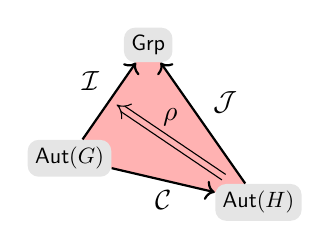
\begin{tikzpicture}[scale=0.8]
  \coordinate (t) at (0,0);
  \coordinate (b) at (-1.25,-1.8);
  \coordinate (d) at (1.75,-2.5);

  \fill[color=red!30] (t) -- (b) -- (d) -- cycle;

  \node[scale=0.8, rounded corners, fill=black!10] (Grp) at (t) {$\cat{Grp}$};
  \node[scale=0.8, rounded corners, fill=black!10] (G) at (b) {$\cat{Aut}(G)$};
  \node[scale=0.8, rounded corners, fill=black!10] (K) at (d) {$\cat{Aut}(H)$};

  \draw (G) edge[->, "{$\fI$}"{name=I, above left}, thick] (Grp);
  \draw (K) edge[->, "{$\fJ$}"{above right}, thick] (Grp);
  \draw (G) edge[->, "{$\func{C}$}"{below}, thick] (K);

  \draw[Rightarrow] (1.2,-2.1) -- (-0.5,-0.95) node[midway, above, yshift=2pt] {$\rho$};
\end{tikzpicture}
\end{center}

We now generalize the notion of a characteristic subgroup to an arbitrary
eastern algebra. Let $\acat{A}$ be a subcategory of an eastern variety
$\acat{E}$. For $G:\acat{E}$, let $\acat{A}(G)$ be the category with a single
object $G$ and morphisms $\acat{A}_1(G, G)$, 
so $\Autcat(G) = \lcore{Grp}(G)$. 
Observe that $\acat{A}(G)$ is a full subcategory of $\acat{A}$.

\begin{defn}\label{def:A-invariance}
  Let $G,H:\acat{E}$, and let $\fI: \acat{A}(G) \to \acat{A}$ and $\fJ :
  \acat{A}(H) \to \acat{A}$ be inclusions. A monomorphism $\iota :
  H\hookrightarrow G$ is \emph{$\acat{A}$-invariant} if there is a functor $\fC:
  \acat{A}(G) \to \acat{A}(H)$ and a monic counital $\eta : \func{JC}
  \Rightarrow \fI$ such that $\eta_G$ is equivalent to $\iota$ (see Section~\ref{sec:subobjects-images} for the definition of equivalence).
\end{defn}

Using the language of Definition~\ref{def:A-invariance}, a characteristic
subgroup $H$ of a group $G$ determines and is determined by a
$\lcore{Grp}$-invariant monomorphism $H\hookrightarrow G$. For fully invariant
subgroups, the corresponding monomorphism is $\acat{Grp}$-invariant.


\subsection{The extension problem and representation theory}
\label{sec:ext-prob}

In Section~\ref{sec:nat-trans-express}, we observed that a characteristic
subgroup $H$ of $G$ determines a functor $\fC : \acat{A} \to\acat{B}$ and a
natural transformation $\rho : \func{JC}\Rightarrow \func{I}$, where $\acat{A}$
and $\acat{B}$ are categories with one object, namely $G$ and $H$ respectively.
If a group $\acute{G}$ is isomorphic to
$G$, then by Fact~\ref{fact:aut-iso} $\acute{G}$ has a characteristic subgroup corresponding to $H$. It
seems plausible that we may be able to extend the functor $\func{C}$ to more
groups and, hence, to larger categories. We now make this notion of extension
precise and generalize it to the setting of eastern algebras.

Fix an eastern variety $\acat{E}$.
Let $\acat{A}$, $\acat{B}$, and $\acat{C}$ be subcategories of 
$\acat{E}$ where $\acat{A} \leq \acat{C}$.
We have inclusion functors $\fI:\acat{A}\to \acat{E}$,
$\fJ:\cB\to \cE$, $\fK:\acat{C}\to \acat{E}$ and $\fL:\acat{A}\to \acat{C}$,
where $\fI=\fK\fL$.  Suppose that  $\rho:\fJ\fC\Rightarrow \fI$ is a monic
counital as depicted in Figure~\ref{fig:char-ext-2-cells}(a). The extension problem
asks whether there is a functor $\fD:\acat{C}\to \acat{E}$ and a natural
transformation $\sigma:\fD\Rightarrow \fK$ such that 
\begin{align}\label{eqn:extension-nat-trans}
  \rho_X = \sigma_{\fL(X)}\tau_X
\end{align}
for some invertible morphism $\tau_X : \func{JC}(X) \to
\func{DL}(X)$ for all objects $X$ of $\acat{A}$. This is depicted in Figure~\ref{fig:char-ext-2-cells}(b).

\begin{figure}[!htbp]
  \pgfmathsetmacro{\rad}{1.5}
  \begin{subfigure}[t]{0.49\textwidth}
    \centering
      \begin{tikzpicture}
        \fill[color=blue!30] (0,0) circle (1.02*\rad cm);
      
        \node[scale=0.8, rounded corners, fill=black!10] (G) at (-\rad, 0) {$\cat{A}$};
      
        \node[scale=0.8, rounded corners, fill=black!10] (B) at (0, -\rad) {$\cat{B}$};

        \node[scale=0.8, rounded corners, fill=black!10] (Grp) at (\rad, 0) {$\cat{E}$};
      
        \node (BB) at (0, -\rad + 0.125*\rad) {};
      
        \draw[very thick, color=black,->] (G) edge[
          out=84, in=97, looseness=1.5, 
          "$\fI$"{below,name=I}] (Grp);
        \draw[very thick,->] (G) edge[
          out=-84, in=173, looseness=1.05, 
          "$\fC$"{left}] (B);
          \draw[very thick,->] (B) edge[
          out=7, in=-97, looseness=1.05, 
          "$\fJ$"{right}] (Grp);
      
        \draw (BB) edge[
            arrows=-Implies,
            double distance=3pt,
            scaling nfold=2, 
            "$\rho$"{right, name=Iota}, pos=0.5, yshift=1em] (I);
      \end{tikzpicture}
    \caption{A diagram of a counital}
    \label{fig:counital-plane}
    \end{subfigure}
    \hfill
    \begin{subfigure}[t]{0.49\textwidth}
      \centering
        \begin{tikzpicture}
          \fill[color=blue!30] (0,0) circle (1.02*\rad cm);
          \fill[color=red!30] (0.5*\rad,0) circle (0.52*\rad cm);
        
          \node[scale=0.8, rounded corners, fill=black!10] (A) at (-\rad, 0) {$\cat{A}$};

          \node[scale=0.8, rounded corners, fill=black!10] (B) at (0, -\rad) {$\cat{B}$};
          \node (BB) at (0, -\rad + 0.125*\rad) {};
        
          \node[scale=0.8, rounded corners, fill=black!10] (C) at (0, 0) {$\cat{C}$};
        
          \node[scale=0.8, rounded corners, fill=black!10] (E) at (\rad, 0) {$\cat{E}$};
        
          \draw[very thick, color=black,->] (A) edge["$\fL$", pos=0.2] (C);
        
          \draw[very thick, color=black,->] (A) edge[
            out=84, in=97, looseness=1.5, 
            "$\fI$"{below,name=I}] (E);
          \draw[very thick,->] (A) edge[
            out=-84, in=173, looseness=1.05, 
            "$\func{C}$"{below}] (B);
          \draw[very thick,->] (B) edge[
            out=7, in=-97, looseness=1.05, 
            "$\fJ$"{right}] (E);
        
          \draw[very thick, color=black,->] (C) edge[
            out=81, in=99, looseness=1.3, 
            "$\fK$"{below,name=K}] (E);
          \draw[very thick,->] (C) edge[
            out=-81, in=-99, looseness=1.3, 
            "$\fD$"{below}, 
            ""{name=D, outer sep=2pt}] (E);
        
          \draw (D) edge[
              arrows=-Implies,
              double distance=3pt,
              scaling nfold=2, 
              "$\sigma$"{right, name=Kappa}, pos=0.4] (K);
          \draw (BB) edge[
            out=135, in=-120,
            arrows=-Implies,
            double distance=3pt,
            scaling nfold=2, 
            "$\tau$"{right, name=Tau}, pos=0.4] (C);
          \draw (C) edge[
            out=135, in=-120,
            arrows=-Implies,
            double distance=3pt,
            scaling nfold=2, 
            pos=0.4] (I);
            \end{tikzpicture}
      \caption{A diagram of an extension}
      \label{fig:ext-rho}
  \end{subfigure}
  \caption{Extending a counital}
  \label{fig:char-ext-2-cells}
\end{figure}

For now, we are concerned only with the existence and construction of such extensions. For use
within an isomorphism test, it will be necessary to develop tools to compute
efficiently with categories; the data types of Section~\ref{sec:comp-nat-trans}
are designed for that purpose.

In light of Proposition~\ref{prop:nat-trans-biact}, we can explore the natural
transformations from Figure~\ref{fig:char-ext-2-cells} through the lens of actions.
Recall that concatenation always denotes regular actions. The natural transformation
$\rho$ defined above is encoded as an $\cA$-bimorphism $\fR:\cA\to \cE$, where
$\rho=\fR(\one_{\cA})$, and this bimorphism defines a cyclic $\cA$-bicapsule
$\Delta\defeq \cA\rho \cdot \cA$ via \eqref{eqn:cyclic-bicap}, which we fix
throughout.

Our goal in part is to extend the cyclic $\cA$-bicapsule $\Delta$ to a cyclic
$\cC$-bicapsule $\Sigma$. Specifically, we will define $\Sigma\defeq\cC \sigma
\cdot \cC$, where $\sigma : \func{D} \Rightarrow \func{K}$ is depicted in
Figure~\ref{fig:char-ext-2-cells}(b).  This is the content of
Theorem~\ref{thm:extension}, but given in  the general setting of eastern algebras. By
construction (Proposition~\ref{prop:nat-trans-biact}), the left actions on
$\Delta$ and $\Sigma$ are regular; hence, we focus on right actions.

\begin{ex}\label{ex_ringstuff}
For the purposes of illustration, we consider 
a familiar construction that is similar to our context, 
namely Frobenius reciprocity and Morita
condensation \cite[Theorem 25A.19]{Rowen}. 
Here $E$ is a ring, and $A$ and $C$ are subrings. Considering 
a Peirce decomposition of $E$, let $\one_A$ and $\one_C$ be
idempotents in $E$ such that
$\one_A\one_C=\one_A=\one_C\one_A$. Then $C= \one_C E\one_C$ is a
(non-unital) subring of $E$, and $A= \one_A E\one_A$ is a subring of both
$C$ and $E$. Furthermore, $\one_A E\one_C=\one_A C$ is an $(A,C)$-bimodule and
$C\one_A=\one_C E\one_A$ is a $(C,A)$-bimodule. Suppose $\Delta$ is a right
$A$-module and $\Sigma$ a right $C$-module. 
The theory of induction and restriction provides us, respectively, 
with a right $C$-module and a right $A$-module: namely, 
\begin{equation*}
  \mathrm{Ind}^C_A(\Delta) \defeq \Delta\otimes_A (\one_A C)\quad\text{and}\quad \mathrm{Res}^C_A(\Sigma) \defeq\Sigma\otimes_C (C\one_A).
\end{equation*}
Thus, $A\to (\one_A C)\otimes_C (C\one_A)$ yields a map
$\Delta\cong\Delta\otimes_A A\to \mathrm{Res}_A^C(\mathrm{Ind}_A^C(\Delta))$.
If, for example, $C\one_A C=C$, then $\Delta \cong
\mathrm{Res}_A^C(\mathrm{Ind}_A^C(\Delta))$.~\exqed
\end{ex}

Guided by the Peirce decomposition from Example~\ref{ex_ringstuff}, we seek similar
constructions for categories and capsules.  Recall that $\cE$ contains a
subcategory $\cC$ that contains a subcategory~$\cA$.  This containment implies
that $\one_{\cA}$ is contained in (rather embeds under the inclusion functors into)
$\one_{\cC}$. The bicapsule action of $\cA$ on $\Delta$ induces a
$\cC$-bicapsule, denoted $\mathrm{Ind}_{\cA}^{\cC}(\Delta)$.  By mimicking
modules, we can consider a formal extension process. We form the type
$\Delta\otimes_{\cA}\cC$ whose terms are 
pairs, denoted $\delta \otimes c$ for $\delta:\Delta$ and $c:\cC$, subject to the equivalence
relation $(\delta\cdot a)\otimes c=\delta \otimes (ac)$. Then we equip this type
with the right $\cC$-action $(\delta\otimes c)\cdot c'=\delta \otimes (cc')$. Defining $ \cA\backslash \cC \defeq \{\cA c \mid c:\cC\}$, we write
\begin{align*}
  \Delta\otimes_{\cA} \cC &= \coprod_{\cA c:\cA\backslash \cC}\Delta\otimes_{\cA} \cA c . 
\end{align*}
We return to this construction in Section~\ref{sec:compose}.
\noindent
Finally, since $\Delta = \cA\rho\cdot \cA$ and $\cC$ are both subtypes of $\cE$,
the product in $\cE$ defines a map $\Delta\times \cC\to \cE$ that factors
through $\Delta\otimes_{\cA}\cC$.  The image of the map is a cyclic
$\cC$-bicapsule $\Sigma$ embedded in $\cE$, with corresponding
$\acat{C}$-bimorphism $\func{S}:\acat{C}\to\acat{E}$.   
The following theorem
states that this is always possible if $\acat{A}$ is full in $\acat{C}$. 
Table~\ref{tab_setup_exthm}  summarizes some of the notation fixed 
throughout this section.

  
\begin{table}[!htb]
  \begin{center}
  \begin{tabular}{l|p{1.5in}}
    $\cE$ & eastern variety\\
    $\cB,\cC$ &  subcategories of $\cE$\\
    $\cA$ & full subcategory of $\cC$
  \end{tabular}
\end{center}
  \renewcommand\arraystretch{1.3}
  \begin{center}
\begin{tabular}{c|c|c}
  bimorphism & monic counital & cyclic bicapsule\\\hline
  $\mathcal{R}: \cat{A}\to\cat{E}$ &  $\rho=\func{R}(\one_{\acat{A}})$ & $\Delta=A\rho\cdot A$\\
  $\mathcal{S}: \cat{C}\to\cat{E}$ &  $\sigma=\func{S}(\one_{\acat{C}})$ & $\Sigma=C\sigma\cdot C$
\end{tabular}
\end{center}
\caption{Data for the proof of Theorem~\ref{thm:extension}}
\label{tab_setup_exthm}
\end{table}


\begin{thm}[Extension]\label{thm:extension}
  Let $\acat{E},\acat{C},\acat{A},\Delta$ be as in Table~$\ref{tab_setup_exthm}$. 
  If $\acat{A}$ is full in $\acat{C}$, then 
there is a cyclic $\cC$-bicapsule $\cat{\Sigma}$ on $\cE$ and unique
  cyclic $\cA$-bicapsules $\cat{\Upsilon}$, $\cat{\Lambda}$ on $\cE$ such that 
\[
    \Delta = \mathrm{Res}_{\cA}^{\cC}(\Sigma)\otimes_{\cA}\Upsilon\quad\text{and}\quad
    \mathrm{Res}_{\cA}^{\cC}(\Sigma) = \Delta \otimes_{\acat{A}} \Lambda.
\]
\end{thm}






We briefly describe the idea of the proof. We start with a cyclic
$\cA$-bicapsule $\Delta$ with associated $\acat{A}$-bimorphism $\fR:\cA\to \cE$.
We seek an extension of $\func{R}$ to a $\acat{C}$-bimorphism $\func{S}\colon
\cat{C}\to \cat{E}$ that
satisfies $\func{S}\func{L}=\func{R}$, where
$\func{L}\colon \acat{A}\to\acat{C}$ is the inclusion functor. If this holds,
then, for every $e:\one_{\acat{A}}$ and every $c:\acat{C}$ with
$\src{c}=\tgt{\func{R}(e)}$,
\[c\cdot\func{R}(e)= c\cdot \func{S}\func{L}(e)=\func{S}(c\cdot
e)=\func{S}(c)=\func{S}(\tgt{c})\cdot c.\]
We now derive some necessary conditions for a putative $\func{S}$ of this type. Recall from \eqref{eq:pre-order} that
the notation $\alpha\ll \beta$ for morphisms $\alpha$ and $\beta$ implies that
there is a morphism $\gamma$ such that $\alpha=\beta\gamma$. Applying
Lemma~\ref{lem:im-monic} to $c\cdot \func{R}(e)=\func{S}(\src{c})\cdot c$ yields
$\mathrm{im}(c\cdot \func{R}(e))\ll \mathrm{im}(\func{S}(\tgt{c}))$. 
For $f:\one_{\acat{C}}$ define
\begin{align*}
\mathbb{U}_{\acat{C}}(f)
\defeq \bigsqcup_{e:\one_{\acat{A}}}f\acat{C}\cdot e.
\end{align*} 
The
  left $\acat{A}$-actions on $\acat{C}$ and $\acat{E}$ are regular, as is
  the left $\acat{C}$-action on $\acat{E}$. 
Hence, for $\langle e,c\rangle:\mathbb{U}_{\acat{C}}(f)$, 
  \[ 
    c\lhd = \src{(c\cdot \one_{\acat{E}})} = (\src{c})\cdot \one_{\acat{E}} = e\cdot \one_{\acat{E}}.
  \]
  Therefore, $c\lhd = e\cdot \one_{\acat{E}} = \tgt{(e\cdot \fR(e))} =
  \tgt{\fR(e)} = \lhd \fR(e)$, so $c\cdot \fR(e)$ is defined. Since
  $\mathrm{im}(c\cdot \func{R}(e))\ll \mathrm{im}(\func{S}(f))$ holds for every
  $\langle e,c\rangle:\mathbb{U}_{\acat{C}}(f)$, we can make a single inclusion (see \eqref{eq:coprod_im_comment}):
\begin{equation}\label{eq_Sdef}
  \mathrm{im}\left(\coprod_{{\langle e,c\rangle \in \mathbb{U}_{\acat{C}}(f)}} \mathrm{im}(c\cdot \func{R}(e))\right) \ll \mathrm{im}(\func{S}(f)).
\end{equation} 
Observe that \eqref{eq_Sdef} also holds if, instead of $\func{R}=\func{SL}$,
we assume that there exists $\func{T}:\acat{A}\to\acat{E}$ such that
$\func{R}(a)=\mathrm{Res}_{\acat{A}}^{\acat{C}}(\func{S})(a)\func{T}(\src{a})$
for all $a:\acat{A}$; here $\mathrm{Res}_{\acat{A}}^{\acat{C}}(\func{S})(a)=\func{S}(\one_{\acat{C}}\cdot a)$ denotes the restriction of $\func{S}$ to $\acat{A}$. This motivates us to choose $\func{S}$ such that
$\func{S}(c)$ is defined as the left hand side of \eqref{eq_Sdef}, and then solve
for a suitable~$\func{T}$.   




In the language of bimorphisms,  Theorem~\ref{thm:extension} asserts that there
exists an $\acat{A}$-bimorphism $\func{T}\colon \acat{A}\to\acat{E}$ such that,
for $a:\acat{A}$,
\begin{align}\label{eqn:RST-bimorphisms}
  \fR(a) &= \fS(\one_{\acat{C}} \cdot (\tgt{a})) \func{T}(a)
  =\fS(\one_{\acat{C}} \cdot a) \func{T}(\src{a})
\end{align}
where $\func{S}$ is the $\acat{C}$-bimorphism corresponding to $\Sigma$; we use
this language in its proof. The second equality in~\eqref{eqn:RST-bimorphisms}
reflects the tensor product over $\cat{A}$ shown in Theorem~\ref{thm:extension}.  


\subsection{Building blocks}\label{sec:blocks}

We prove Theorem~\ref{thm:extension} in Section~\ref{sec:extension-proof} using the three
intermediate results presented in this section.\enlargethispage{0.5cm}

\begin{lem}\label{lem:S-sufficient}
Let $\cC$ and $\cE$ be as in Table~$\ref{tab_setup_exthm}$. 
  For  $\sigma:\prod_{f:\one_{\cC}}(f~\cdot\mono{E})$, the
  following are equivalent. 
  \begin{ithm}
    \item[\rm (1)] There is a $\cC$-bicapsule $\Sigma$ on $\cE$ such that the
    function $\fS : \cC \to \Sigma$ given by 
    \(
      \fS(c) \defeq c\cdot \sigma_{\src{c}}
    \)
    is a $\cC$-bimorphism. 

    \item[\rm (2)] For all $c:\acat{C}$, $c\cdot \sigma_{\src{c}} \ll
    \sigma_{\tgt{c}}$.
  \end{ithm}
\end{lem}

\begin{proof}
  We assume (1) holds and prove (2). By
  Proposition~\ref{prop:nat-trans-biact}\ref{proppart:get-nat-trans}, there exists a unique
  functor $\func{G} : \acat{C}\to \acat{E}$ that induces the action of
  $\acat{C}$ on the right of $\acat{E}$. Since $\fS$ is a function and a 
  $\cC$-bimorphism by assumption, $c\lhd= \lhd \sigma_{\src{c}}$ for all
  $c:\acat{C}$, and 
  \begin{align*}
    c\cdot \sigma_{\src{c}} 
    & = \fS(c) =\fS((\tgt c)\cdot c)= \fS(\tgt{c})\cdot c
    = ((\tgt{c}) \cdot \sigma_{\src{(\tgt{c})}}) \cdot c  
    =\sigma_{\tgt{c}}\fG(c) . 
  \end{align*}
  Thus, (2) holds.

  We now assume (2) holds and prove (1). First, we show that an $x:\acat{E}$
  satisfying $c\cdot \sigma_{\src{c}} = \sigma_{\tgt{c}}x$ is unique. Suppose
  $y:\acat{E}$ satisfies $c\cdot \sigma_{\src{c}} = \sigma_{\tgt{c}}y$, so
  $\sigma_{\tgt{c}}x = \sigma_{\tgt{c}}y$. Since $\sigma_{\tgt{c}}$ is a
  monomorphism, $x=y$. We denote this unique morphism by $u_c:\acat{E}$. Since
  $\sigma_{\tgt{c}}u_c$ is defined for all $c:\cC$, 
  \begin{align*}
    \tgt{u_{\tgt{c}}} = \src{(\sigma_{\tgt{(\tgt{c})}})} 
    = \src{(\sigma_{\tgt{c}})} = \tgt{u_c}.
  \end{align*}
  Next, we define a right $\cC$-capsule structure on $\acat{E}$ as
  follows. Let $\lhd (-) : \cC \to \one_{\cE}$ be given by $\lhd c =
  \tgt{u_c}$, and let $(-)\lhd : \cE \to \one_{\cE}$ be given by
  $x\lhd = \src{x}$. For all $c:\cC$ and $x:\cE$, let $x\cdot c =
  xu_c$, which is defined if, and only if, $\src{x} = \tgt{u_c}$. Condition (2)
  of Definition~\ref{def:cat-act} follows from $\lhd (\tgt{c}) = \tgt{u_{\tgt{c}}} =
  \tgt{u_c} = \lhd c$ and $u_e:\one_{\cE}$ for all $e:\one_{\cC}$
  since $\sigma_e$ is monic. Lastly, let $c,d:\cC$ with $\src{c}=\tgt{d}$.
  Then $(cd) \cdot \sigma_{\src{(cd)}} = \sigma_{\tgt{(cd)}}u_{cd} =
  \sigma_{\tgt{c}}u_{cd}$ and, since we have a regular left action,  
  \begin{align*}
    (cd) \cdot \sigma_{\src{(cd)}}  
    = c \cdot (d \cdot \sigma_{\src{(cd)}})
    = c\cdot (d\cdot \sigma_{\src{d}}) 
    = c\cdot \sigma_{\tgt{d}} u_d 
    = \sigma_{\tgt{c}}u_cu_d.
  \end{align*}
  Since $\sigma_{\tgt{c}}$ is a monomorphism, $u_{cd}=u_cu_d$. Hence, this
  defines a right $\cC$-capsule on $\cE$ since $\lhd c = \tgt{u_c}:\one_{\cE}$
  for all $c:\cC$. Since $\acat{C}$ acts regularly on $\acat{E}$ on the left,
  there exists a $\acat{C}$-bicapsule $\Sigma$ on $\acat{E}$ by
  Proposition~\ref{prop:functors-are}, with the regular left and right actions
  just defined. Finally, we prove that $\fS$ is a $\cC$-bimorphism. For all
  $c,x,y:\cC$, 
  \begin{align*}
    \func{S}(cx) &= (cx)\cdot \sigma_{\src{(cx)}} 
    = (cx)\cdot \sigma_{\src{x}} 
    = c\cdot (x\cdot \sigma_{\src{x}}) 
    = c\cdot \fS(x),
  \end{align*}
  provided $\src{c}=\tgt{x}$. If $\src{y} = \tgt{c}$, then 
  \begin{align*}
    \fS(yc) &= (yc)\cdot \sigma_{\src{(yc)}} 
    = (yc)\cdot \sigma_{\src{c}} 
    = y\cdot (c\cdot \sigma_{\src{c}}) 
    = y\cdot (\sigma_{\tgt{c}}u_c)
    = (y\cdot \sigma_{\src{y}})u_c \\
    &= \fS(y)\cdot c.\qedhere
  \end{align*}
\end{proof}
\enlargethispage{0.7cm}


\begin{lem}\label{lem:def-sigma}
For $\acat{E},\acat{C},\func{R}$ as in Table~$\ref{tab_setup_exthm}$,  
define $\sigma :
  \coprod_{f:\one_{\acat{C}}}(f~\cdot \mono{E})$ via
  \begin{equation*} 
    \sigma_{f}  \defeq \mathrm{im}\left(
      \coprod_{\langle e,x\rangle:\mathbb{U}_{\acat{C}}(f)} 
        \mathrm{im}(x\cdot \fR(e))
        \right). 
  \end{equation*}
  For each $c:\acat{C}$, there is a unique $y:\acat{E}$ satisfying $c\cdot
  \sigma_{\src{c}}=\sigma_{\tgt{c}}y$.
\end{lem}


\begin{proof}
Let $c:\acat{C}$, so $c \lhd = \src{c}$, and $\src{c} = \lhd \sigma_{\src{c}}$
  by definition of $\sigma$. We show that $c\cdot \sigma_{\src{c}}
  \ll\sigma_{\tgt{c}}$. By Lemma~\ref{lem:im}, 
  \begin{align*} 
    &(\forall \langle e,x\rangle:\mathbb{U}_{\acat{C}}(f))&  c\cdot \mathrm{im}(x\cdot \fR(e))& \ll\mathrm{im}(c\cdot (x\cdot \fR(e))) = \mathrm{im}((cx)\cdot \fR(e)).
  \end{align*}
  Thus, by Fact~\ref{fact:coprod}\ref{factpart:ignore-inside},
  \begin{align}
    \label{eq:coprod-ineq}
    \coprod_{\langle e,x\rangle:\mathbb{U}_{\acat{C}}(f)} \left(c\cdot \mathrm{im}(x\cdot \fR(e))\right)
      &\ll \coprod_{\langle e,x\rangle:\mathbb{U}_{\acat{C}}(f)} \mathrm{im}((cx)\cdot \fR(e)).
  \end{align}
  Therefore, using \eqref{eq:coprod_im_comment},
\begin{align*}
  c\cdot \mathrm{im}\left(
    \coprod_{\langle e,x\rangle}
        \mathrm{im}(x\cdot \fR(e))
  \right) 
  & \ll  \mathrm{im}\left(
    c\cdot 
    \coprod_{\langle e,x\rangle}
        \mathrm{im}(x\cdot \fR(e))
  \right) & & (\text{Lemma~\ref{lem:im}}) \\
  & =  \mathrm{im}\left(
    \coprod_{\langle e,x\rangle}
      (c\cdot 
        \mathrm{im}(x\cdot \fR(e)))
  \right) & & (\text{Fact~\ref{fact:coprod}\ref{factpart:factor-out}}) \\
  & \ll  \mathrm{im}\left(
    \coprod_{\langle e,x\rangle}
        \mathrm{im}((cx)\cdot \fR(e))
  \right) & & (\text{Equation (\ref{eq:coprod-ineq})}) 
\end{align*} 
where all of the coproducts are over
$\langle e,x\rangle:\mathbb{U}_{\acat{C}}(\src{c})$. By 
Fact~\ref{fact:coprod}\ref{factpart:smaller-coprod}, 
\[ 
  \mathrm{im}\left(
    \coprod_{\langle e,x\rangle:\mathbb{U}_{\acat{C}}(\src{c})}
        \mathrm{im}((cx)\cdot \fR(e))
  \right) \ll \mathrm{im}\left(
        \coprod_{\langle e,z\rangle:\mathbb{U}_{\acat{C}}(\tgt{c})} 
          \mathrm{im}(z\cdot \fR(e))
    \right).
\]
Putting this together, we deduce that 
\begin{align*}
  c\cdot \sigma_{\src{c}} &= c\cdot \mathrm{im}\left(
    \coprod_{\langle e,x\rangle:\mathbb{U}_{\acat{C}}(\src{c})}
        \mathrm{im}(x\cdot \fR(e))
  \right) 
  \ll \mathrm{im}\left(
    \coprod_{\langle e,z\rangle:\mathbb{U}_{\acat{C}}(\tgt{c})} 
      \mathrm{im}(z\cdot \fR(e))
\right) = \sigma_{\tgt{c}}, 
\end{align*}
so $c\cdot \sigma_{\src{c}}=\sigma_{\src{c}}y$ for some $y:\acat{E}$. Since
$\sigma_{\tgt{c}}$ is monic, $y$ is unique. 
\end{proof}

 
\begin{prop}\label{prop:T}
 Let $\acat{E},\acat{C},\acat{A},\func{R}$ be as in Table~$\ref{tab_setup_exthm}$. 
If $\acat{A}$ is full in $\acat{C}$, 
 then $\func{S}: \acat{C}\to\acat{E}$ defined by 
  \[\func{S}(c)\defeq c\cdot \mathrm{im}\left(\coprod_{\langle e,x\rangle:\mathbb{U}_{\acat{C}}(\src{c})} \mathrm{im}(x\cdot\func{R}(e))  \right)\]
   is a  $\acat{C}$-bimorphism, and there exists a unique
  $\lambda:\prod_{f:\one_{\acat{A}}}f\!\!\core{E}\!\!f$ such that for all $a:\acat{A}$,  
  \begin{equation*}
    \fR(a) = \fS(a \cdot\one_{\acat{C}}) \lambda_{\src{a}}\quad\text{and}\quad \fS(a \cdot\one_{\acat{C}}) = \fR(a) \lambda_{\src{a}}^{-1}. 
  \end{equation*}
\end{prop}

\begin{proof}
  Take $e,f:\one_{\acat{A}}$, and recall that $\acat{A}$ acts regularly on both
  the left and right of $\acat{C}$. Since $\acat{A}$ is full in $\acat{C}$, 
these actions are full, so 
  \[
    f\cdot\acat{C}\cdot e = \one_{\acat{C}} \cdot (f\acat{A}e) = (f\acat{A}e) \cdot \one_{\acat{C}} . 
  \]
  Since the left actions of $\acat{A}$ on $\acat{C}$ and on $\acat{E}$ 
and the left action of $\acat{C}$ on $\acat{E}$ are regular, for each
  $a:\acat{A}$ and $x:\acat{E}$ with $a\lhd = \lhd x$,
  \begin{align}\label{eqn:C-to-A}
    (a\cdot \one_{\acat{C}}) \cdot x &= a\cdot x. 
  \end{align}
  Fix $a:\acat{A}$. Set $c = a\cdot\one_{\acat{C}}$, so $(\src{c})\acat{C} = (\src{a})\cdot
  \acat{C}$. Thus, since the $\acat{A}$-action on $\acat{C}$ is full,
  \begin{align}\label{eqn:subscripts}
    \mathbb{U}_{\acat{C}}(\src{c}) \defeq \bigsqcup_{e:\one_{\acat{A}}} \left((\src{c})\acat{C}\cdot e\right) &= \bigsqcup_{e:\one_{\acat{A}}} \left((\src{a})\cdot \acat{C}\cdot e\right) = ((\src{a})\acat{A})\cdot \one_{\acat{C}},
  \end{align}
  where $(\src{a})\acat{A}$ acts on $\one_{\acat{C}}$ in the final expression.
  Therefore, 
  \begin{align*}
    \fS(a\cdot\one_{\acat{C}}) 
    & = a\cdot \mathrm{im}\left(\coprod_{\langle e,x\rangle:\mathbb{U}_{\acat{C}}((\src{a})\cdot \one_{\acat{C}})} \mathrm{im}(x\cdot \fR(e))\right) 
        & & (\text{Equation \eqref{eqn:C-to-A}}) \\ 
    & = a\cdot \mathrm{im}\left(\coprod_{a':(\src{a})\acat{A}} \mathrm{im}(a'\cdot \fR(\src{a'}))\right) 
        & & (\text{Equation \eqref{eqn:subscripts}})\\
    & = a\cdot \mathrm{im}\left(\coprod_{a':(\src{a})\acat{A}} \mathrm{im}(\fR(\src{a})\cdot a')\right) 
        & & (\text{$\acat{A}$-bimorphism, $\tgt{a'} = \src{a}$})\\
    & \ll a\cdot \fR(\src{a}) = \fR(a).
    & & (\text{Lemma~\ref{lem:im-monic},  Fact~\ref{fact:coprod}\ref{factpart:factor-out}})
  \end{align*}
\noindent 
For the application of Lemma~\ref{lem:im-monic} in the last step, recall that 
$\func{R}(e)$ is monic for $e:\acat{A}$ by our assumption 
(Table~\ref{tab_setup_exthm}). 

We establish the other direction as follows:
  \begin{align*}
    \fR(\src{a}) &\ll \mathrm{im}(\fR(\src{a})) = \mathrm{im}((\src{a})\cdot \fR(\src{a})) & & (\text{Theorem~\ref{thm:Noether}}) \\
    &\ll \coprod_{a':(\src{a})\acat{A}} \mathrm{im}(a' \cdot \fR(\src{a'})) & & (\text{Fact~\ref{fact:coprod}\ref{factpart:smaller-coprod}}) \\
    &\ll \mathrm{im}\left(\coprod_{a':(\src{a})\acat{A}} \mathrm{im}(a' \cdot \fR(\src{a'}))\right). & & (\text{Theorem~\ref{thm:Noether}}) 
  \end{align*}
  Acting with $a:\acat{A}$ from the left, we obtain $\fR(a) \ll \fS(a\cdot \one_{\acat{C}})$.

  From both computations, there exist $\lambda,\mu : \prod_{f:\one_{\acat{A}}}
  f\acat{E}f$ such that 
  \begin{align*}
    \fR(a) &= \fS(a \cdot\one_{\acat{C}}) \lambda_{\src{a}}, 
    & \fS(a \cdot\one_{\acat{C}}) &= \fR(a) \mu_{\src{a}}. 
  \end{align*}
  It remains to show that $\mu_{\src{a}} = \lambda_{\src{a}}^{-1}$ for all
  $a:\acat{A}$ and $\lambda$ is unique. For all $e:\one_{\acat{A}}$, 
  $\fR(e)$ is monic by the assumptions in Theorem~\ref{thm:extension}, and 
  $\fS(e\cdot \one_{\acat{C}})$ is also monic by the definition of $\fS$.
  Since $\fR(e)$ is monic, 
  \begin{align*}
    \fR(e) &= \fS(e \cdot\one_{\acat{C}}) \lambda_{e} = \fR(e)\mu_{e}\lambda_{e}
  \end{align*}
  implies $\mu_{e}\lambda_{e} : \one_{\acat{E}}$. Similarly, $\lambda_{e} \mu_{e}
  : \one_{\acat{E}}$ because $\fS(e\cdot\one_{\acat{C}})$ is monic and
  \begin{align*}
    \fS(e \cdot\one_{\acat{C}}) &= \fR(e) \mu_{e} = \fS(e \cdot\one_{\acat{C}}) \lambda_{e} \mu_{e} .
  \end{align*}
  The uniqueness of $\lambda$ follows since $\fR(e)$ is monic.
\end{proof}



\subsection{Proof of Theorem~\ref{thm:extension}}
\label{sec:extension-proof}
Let $\fS : \acat{C} \to \acat{E}$ be the $\acat{C}$-bimorphism in Proposition~\ref{prop:T}. 
This proposition shows that there exists a unique
$\lambda:\prod_{f:\one_{\acat{A}}}f\!\!\core{E}\!\!f$ such that for all
$a:\acat{A}$,
\begin{align}\label{eqn:R-lambda}
  \fR(a) &= \fS(a\cdot \one_{\acat{C}}) \lambda_{\src{a}}. 
\end{align}
Since $\fR$ is an $\acat{A}$-bimorphism, 
\begin{align}\label{eqn:S-CC}
  (a\cdot \one_{\acat{E}}) \cdot \fR(\src{a}) &= \fR(a) = \fR(\tgt{a}) \cdot (\one_{\acat{E}}\cdot a).
\end{align}
Let $\Sigma$ be the $\acat{C}$-bicapsule on $\cE$ defined by the
$\cC$-bimorphism $\func{S}$. Both  $\Delta$ and $\Sigma$ are bicapsules, so
applying \eqref{eqn:R-lambda} to \eqref{eqn:S-CC} yields
\begin{align}\label{eqn:baseline}
  (a\cdot \one_{\acat{E}})\fS((\src{a})\cdot \one_{\acat{C}}) \lambda_{\src{a}} &=\fS((\tgt{a})\cdot \one_{\acat{C}}) \lambda_{\tgt{a}}(\one_{\acat{E}}\cdot a).
\end{align}
Since the left $\acat{C}$-action on $\acat{E}$ and the left $\acat{A}$-action on
$\acat{C}$ are regular, $a\cdot \one_{\acat{E}}=(a \cdot \one_{\acat{C}}) \cdot
\one_{\acat{E}}$. Thus, $(a\cdot \one_{\acat{E}})\fS((\src{a})\cdot
\one_{\acat{C}}) = \fS(a\cdot \one_{\acat{C}}) = \fS((\tgt{a})\cdot
\one_{\acat{C}})(\one_{\acat{E}}\cdot (\one_{\acat{C}} \cdot a))$. Applying this
to \eqref{eqn:baseline} and using the monic property of $\fS((\tgt{a})\cdot
\one_{\acat{C}})$, we deduce that
\begin{align*}
  (\one_{\acat{E}}\cdot (\one_{\acat{C}} \cdot a))\lambda_{\src{a}} &= \lambda_{\tgt{a}}(\one_{\acat{E}}\cdot a) . 
\end{align*}
Since the actions are capsules, $\lambda$ defines a natural transformation. 
By Proposition~\ref{prop:nat-trans-biact}\ref{proppart:get-biactions}, the
function $a\mapsto (\one_{\acat{E}}\cdot (\one_{\acat{C}} \cdot
a))\lambda_{\src{a}}$ defines an $\acat{A}$-bimorphism $\func{T} :
\acat{A}\to \acat{E}$. Thus, $\func{T}(\src{a}) = \lambda_{\src{a}} :\,\core{E}$,
and therefore
\begin{align*}
  \fR(a) &= \fS(\one_{\acat{C}} \cdot a) \func{T}(\src{a}) = \fS(\one_{\acat{C}} \cdot (\tgt{a})) (\one_{\acat{E}}\cdot (\one_{\acat{C}} \cdot a)) \func{T}(\src{a}) = \fS(\one_{\acat{C}} \cdot (\tgt{a})) \func{T}(a).
\end{align*}
The uniqueness of $\func{T}$ follows from
Proposition~\ref{prop:nat-trans-biact}\ref{proppart:get-nat-trans} and the uniqueness of
$\lambda$. \qed


\subsection{Proof of Theorem~\ref{thm:char-counital} for eastern varieties}
\label{sec:proofThm1} 

Recall that
$\text{Counital}(\cB,\cE)$ denotes the type of all counitals
$\iota:\func{K}\fC\Rightarrow \fI$, where $\cB\leq \cE$ and $\cat{C}$ are 
categories, $\fC: \cB\to \cC$ is a functor, and $\fI:\cB\to \cE$ and
$\func{K}:\cC\to \cE$ are inclusion functors.   Let $\text{Unital}(\cB,\cE)$ be
the type  of all unitals $\pi:\fI\Rightarrow \fK\fC$; these are the duals of
counitals. Recall from Theorem~\ref{thm:Noether}
that $\mathrm{im}$ and $\mathrm{coim}$ produce categorical morphisms, and from
Section~\ref{sec:subobjects-images} the equivalence relations on monomorphisms
and epimorphisms. Our use of set theory notation in the 
following generalization of Theorem~\ref{thm:char-counital} 
is justified because we compare subsets of a fixed algebra.

\begingroup   
\renewcommand{\themainthm}{1-cat} 
\begin{mainthm}\label{thm:char-counital-eastern}
  Let $\cE$ be an eastern variety. For every $G:\cE$, the following equalities of sets hold up to equivalence:
    \begin{align}
      \tag{1}
      \{\iota:H\hookrightarrow G \mid \iota\text{ is $\core{E}$-invariant} \} 
      & = 
      \left\{
        \text{\rm im}(\eta_G) \mid \eta: \text{\rm Counital}\left(\core{\cE},\cE\right)
      \right\};\\[5pt]
      \tag{2}
      \{\pi:G\twoheadrightarrow Q \mid \pi\text{ is $\core{E}$-invariant} \} 
      & =  
      \left\{
        \text{\rm coim}(\tau_G) \mid \tau: \text{\rm Unital}\left(\core{E},\cE\right)
      \right\};\\[5pt]
      \tag{3}
      \{\iota:H\hookrightarrow G \mid \iota\text{ is $\acat{E}$-invariant} \} 
      & =
      \left\{
        \text{\rm im}(\eta_G) \mid \eta: \text{\rm Counital}(\cat{E},\cE)
      \right\};\\[5pt]
      \tag{4}
      \{\pi:G\twoheadrightarrow Q \mid \pi\text{ is $\acat{E}$-invariant} \} 
      & = 
      \left\{
        \text{\rm coim}(\tau_G) \mid \tau: \text{\rm Unital}(\cat{E},\cE)
      \right\}.
    \end{align}
\end{mainthm}
\endgroup

    
\begin{proof}
 We prove (1) in detail; the proof of (3) is analogous but requires replacing $\core{E}$ with $\cat{E}$. The proofs of (2) and (4) are dual to the proofs of (1) and (3), respectively.

 
Let $\iota : H\hookrightarrow G$, which is a morphism in $\cat{E}$. Recall that
the single-object category $\Autcat(G)$ consists of $G$ and all its
automorphisms,  and likewise for  $\Autcat(H)$. Both are subcategories of
$\cat{E}$, and full subcategories of  $\core{E}$. We denote the relevant
inclusion functors by  $\fI:\Autcat(G)\to \cE$, $\fJ:\Autcat(H)\to \cE$,  
$\fL:\Autcat(G)\to \;\core{E}$, and $\fK:\;\core{E}\;\to \cE$. As in
Section~\ref{sec:nat-trans-express}, we obtain a natural transformation
$\rho:\fJ\fC\Rightarrow \fI$ with (restriction) functor
$\fC:\Autcat(G)\to\Autcat(H)$, so $\rho: \text{Counital}(\Autcat(G),\cE)$ is a
monic counital.

We now use Proposition~\ref{prop:nat-trans-biact} to pass to the associated
cyclic $\Autcat(G)$-bicapsule  $\Delta=\Autcat(G)\cdot \rho\cdot \Autcat(G)$.
Recall that the left action is defined by $\func{I}$, hence regular, and the
right action is defined by $\func{JC}$.  By construction, $\Delta$ satisfies the
conditions of Theorem~\ref{thm:extension} since $\Autcat(G)$ is full in
$\core{E}$. We extend $\Delta$ to a cyclic $\core{E}$-bicapsule
$\Sigma=\core{E}\cdot \sigma \cdot \core{E}$ where $\sigma:\fK\fD\Rightarrow
\fK$ is a monic counital extending $\rho$, namely, there exists an isomorphism
$\tau_G : \func{JC}(G) \to \func{DL}(G)$ such that $\iota =
\rho_G=\sigma_{\func{L}(G)}\tau_G$; see \eqref{eqn:extension-nat-trans}. Since
$\fL$ is the inclusion functor, there exists an isomorphism $\tau':\acat{E}$
such that $\iota = \sigma_G\tau'$, so $\iota$ and $\sigma_G$ are equivalent.
Hence, $\iota$ and $\mathrm{im}(\sigma_G)$ are equivalent. Since
$\sigma:\text{Counital}(\core{E},\cE)$, this proves the ``$\subseteq$'' part of
(1). 

For the converse, consider $\eta: \text{Counital}(\core{E},\cE)$, say $\eta:
\func{HD}\Rightarrow\func{K}$ for some functor $\fD:\; \core{E}\;\to \cat{C}$,
subcategory $\cat{C}\leq\acat{E}$, and inclusion $\func{H}:\cat{C}\to \cE$.  If
$\varphi:\Autcat(G)$, then $\fL(\varphi):\; \core{E}$, and so
$\func{K}\fL(\varphi) \eta_G =\eta_G \func{H}\fD\func{L}(\varphi)$. Since
$G=\func{L}(G)=\func{K}(G)$, it follows that the morphism  $\eta_G:
\func{HD}(G)\to G$ is characteristic, and therefore so is its monic image
$\mathrm{im}(\eta_G)$. This proves the ``$\supseteq$'' part of (1).
\end{proof}

\section{Categorification of characteristic substructure}
\label{sec:inv-cat}

The final step in our work is to 
describe the source of all characteristic subgroups, and more generally 
characteristic substructures in eastern algebras.  
In Section~\ref{sec:induced}, we showed that characteristic structure 
arises naturally from counitals.  Now we demonstrate that all counitals 
are derived from counits. In particular, 
in Section~\ref{sec:proofs}, we prove the following generalization of
Theorem~\ref{thm:char-repn} to eastern algebras.  
\begingroup
\renewcommand{\themainthm}{2-cat} 
\begin{mainthm}\label{thm:char-repn-eastern}
  Fix an eastern variety $\cE$. Let $G$ be an object in $\cE$ with subobject 
$H$ and inclusion $\iota:H\hookrightarrow G$.
   There exist categories $\cat{A}$ and $\cat{B}$, where
   $\core{E}\;\leq\acat{A}\leq\acat{E}$, such that the following are
   equivalent. 
  \begin{ithm}
    \item[\rm (1)] $H$ is characteristic in $G$.
    \item[\rm (2)] There is a functor $\func{C} : \cat{A} \to \cat{A}$ and
     a counit $\eta:\func{C}\Rightarrow \id_{\cat{A}}$ such that 
     $H = \im(\eta_G)$.
    \item[\rm (3)] There is an $(\acat{A},\acat{B})$-morphism $\mathcal{M}:\acat{B}\to
    \acat{A}$ such that $\iota=\mathcal{M}(\id_G \cdot \one_{\acat{B}})$.
  \end{ithm} 
\end{mainthm}
  \endgroup
  
Our proof relies on  the Extension Theorem~\ref{thm:extension} and further
consideration of counitals.

\begin{defn}\label{def:counital-type}
  Fix a category $\cE$ with subcategories $\cat{A}$ and $\cat{B}$ and
  inclusion functors $\func{I} : \cA \to \cE$ and $\func{J} : \cB
  \to \cE$. 
  A counital  $\eta : \func{JC}\Rightarrow \func{I}$ is \emph{isosceles} 
if $\cat{A}=\cat{B}$ and $\fI=\fJ$, and 
    \emph{flat} if, in addition, $\cA=\cB=\cE$ and $\fI=\fJ=\id_{\cE}$. 
Otherwise, it is \emph{scalene}.
\end{defn} 


\begin{ex}\label{ex:three-chars}
  We mention three examples in $\cat{Grp}$ and 
illustrate their natural transformations in 
Figure~\ref{fig:counital}. 
The first two are the derived subgroup and the centre of a group considered 
in Example~\ref{ex:three-chars_first}. For the third example, we consider an 
arbitrary characteristic subgroup $H$ of a group $G$. 
  As discussed in Section~\ref{sec:ext-prob}, define
  $\cat{Aut}(G)$ to be the category with one object $G$ and 
its morphisms are the
  automorphisms of $G$. Hence, $\cat{Aut}(G)$ and $\cat{Aut}(H)$ are
  subcategories of $\cat{Grp}$ with inclusion functors $\func{J}$ and
  $\func{K}$, respectively. We define a functor $\func{C} : \cat{Aut}(G) \to
  \cat{Aut}(H)$ by mapping $G$ to $H$ and automorphisms of $G$ to their
  restriction to $H$, and so obtain a natural transformation $\iota :
  \func{K}\func{C} \Rightarrow \func{J}$.~\exqed
\end{ex}

  




\begin{figure}[!htbp]
  \begin{subfigure}[t]{0.32\textwidth}
    \centering
    \pgfmathsetmacro{\rad}{1.25}
    \begin{tikzpicture}
      \fill[color=ForestGreen!30] (0,0) circle (1.02*\rad cm);
    
      \node[scale=0.8, rounded corners, fill=black!10] (G) at (-\rad, 0) {$\cat{Grp}$};
    
      \node[scale=0.8, rounded corners, fill=black!10] (Grp) at (\rad, 0) {$\cat{Grp}$};
    
      \draw[very thick, color=black,->] (G) edge[
      out=84, in=97, looseness=1.5, 
      "$\id$"{below,name=I}] (Grp);
      \draw[very thick,->] (G) edge[
      out=-84, in=-97, looseness=1.5, 
      "$\func{D}$"{above, name=C}, 
      ] (Grp);
    
      \draw (C) edge[
      arrows=-Implies,
      double distance=3pt, 
      scaling nfold=2, 
      "$\lambda$"{right, name=Iota}, 
      pos=0.4] (I);
    \end{tikzpicture} 
    \caption{The derived subgroup}
    \label{fig:comm-counital}
    \end{subfigure}
    \hfill
  \begin{subfigure}[t]{0.32\textwidth}
	\centering
	\pgfmathsetmacro{\rad}{1.25}
  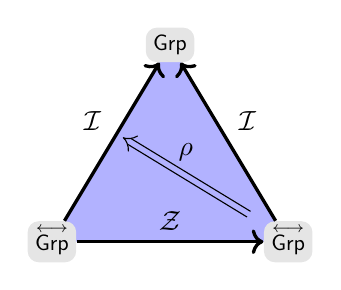
\begin{tikzpicture}
    \coordinate (t) at (0,0);
    \coordinate (b) at (-1.5,-2.5);
    \coordinate (d) at (1.5,-2.5);

    \fill[color=blue!30] (t) -- (b) -- (d) -- cycle;

    \node[scale=0.8, rounded corners, fill=black!10] (Grp) at (t) {$\cat{Grp}$};
    \node[scale=0.8, rounded corners, fill=black!10] (G) at (b) {$\lcore{Grp}$};
    \node[scale=0.8, rounded corners, fill=black!10] (K) at (d) {$\lcore{Grp}$};

    \draw (G) edge[->,"{$\func{I}$}"{name=I, above left}, very thick] (Grp);
    \draw (K) edge[->,"{$\func{I}$}"{above right}, very thick] (Grp);
    \draw (G) edge[->, "{$\func{Z}$}", very thick] (K);

    \draw[Rightarrow] (1,-2.15) -- (-0.6,-1.175) node[midway, above, yshift=2pt] {$\rho$};
  \end{tikzpicture}
	\caption{The center}
	\label{fig:center-counital}
  \end{subfigure}
  \hfill
  \begin{subfigure}[t]{0.33\textwidth}
    \centering
    \pgfmathsetmacro{\rad}{1.25}
    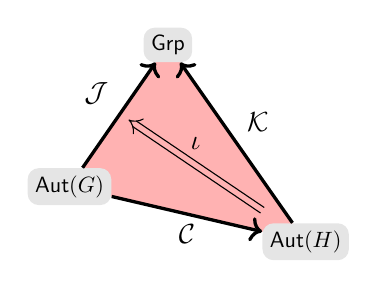
\begin{tikzpicture}
      \coordinate (t) at (0,0);
      \coordinate (b) at (-1.25,-1.8);
      \coordinate (d) at (1.75,-2.5);
  
      \fill[color=red!30] (t) -- (b) -- (d) -- cycle;
  
      \node[scale=0.8, rounded corners, fill=black!10] (Grp) at (t) {$\cat{Grp}$};
      \node[scale=0.8, rounded corners, fill=black!10] (G) at (b) {$\cat{Aut}(G)$};
      \node[scale=0.8, rounded corners, fill=black!10] (K) at (d) {$\cat{Aut}(H)$};
  
      \draw (G) edge[->, "{$\func{J}$}"{name=I, above left}, very thick] (Grp);
      \draw (K) edge[->, "{$\func{K}$}"{above right}, very thick] (Grp);
      \draw (G) edge[->, "{$\func{C}$}"{below}, very thick] (K);
  
      \draw[Rightarrow] (1.2,-2.1) -- (-0.5,-0.95) node[midway, above, yshift=2pt] {$\iota$};
    \end{tikzpicture}
    \caption{A characteristic subgroup}
    \label{fig:single-counital}
    \end{subfigure}  
	\caption{Natural transformations from Example~\ref{ex:three-chars}}
	\label{fig:counital}
\end{figure}


In our study of characteristic structure we consider the three types of
counitals.  First, we use  induced actions from Theorem~\ref{thm:char-from-biacts} to
pass from a scalene counital to one that is isosceles.  Next, we work with
isosceles counitals to determine an intermediate class of isosceles counitals
known as \emph{internal} counitals.  Finally, we show that internal counitals
are completely determined by a morphism of bicapsules.

Counits are common in many categorical contexts; for example, they occur for
every adjoint functor pair.  The case of flat counitals coincides precisely with
the stricter class of fully-invariant substructures.  


\subsection{Composing counitals}

In this section, we describe two ways to construct new counitals from given
counitals by composing natural transformations and functors in different ways. These are two instances of a much larger theory; see \cite{Baez, Power}. Figure~\ref{fig:char-ext-2-cells} illustrates the usual composition
of natural transformations. We now  describe how to compose a functor with a
natural transformation. Consider functors $\func{F},\func{G}:\cat{B}\to
\cat{A}$, $\func{H}:\cat{C}\to\cat{B}$, and $\func{K}:\cat{A}\to \cat{D}$ for
categories $\cat{A}$, $\cat{B}$, $\cat{C}$, and $\acat{D}$, and a natural
transformation $\eta : \func{F} \Rightarrow \func{G}$. Define $\eta
\func{H}:\func{F}\func{H}\Rightarrow \func{G}\func{H}$ by setting $(\eta
\func{H})_X\defeq \eta_{\func{H}(X)}$ for each object $X$ in $\cat{C}$.
Similarly, define $\func{K}\eta:\func{K}\func{F}\Rightarrow \func{K}\func{G}$ by
setting $(\func{K}\eta)_Y\defeq\func{K}(\eta_Y)$ for each $Y$ in $\cat{B}$. The
effects of $\eta \func{H}$ and $\func{K}\eta$ are displayed
in~Figure~\ref{fig:nat-trans-functor}.

\begin{figure}[!htbp]
  \pgfmathsetmacro{\rad}{1.5}
  \begin{subfigure}[t]{0.49\textwidth}
    \centering
      \begin{tikzpicture}
        \fill[color=blue!30] (0,0) circle (1.02*\rad cm);
        \fill[color=red!30] (0.5*\rad,0) circle (0.52*\rad cm);
      
        \node[scale=0.8, rounded corners, fill=black!10] (G) at (-\rad, 0) {$\cat{C}$};
      
        \node[scale=0.8, rounded corners, fill=black!10] (H) at (0, 0) {$\cat{B}$};
      
        \node[scale=0.8, rounded corners, fill=black!10] (Grp) at (\rad, 0) {$\cat{A}$};
      
        \draw[very thick, color=black,->] (G) edge["$\func{H}$", pos=0.2] (H);
      
        \draw[very thick, color=black,->] (G) edge[
          out=84, in=97, looseness=1.5, 
          "$\func{G}\func{H}$"{below,name=I}] (Grp);
        \draw[very thick,->] (G) edge[
          out=-84, in=-97, looseness=1.5, 
          "$\func{F}\func{H}$"{below}, 
          ""{name=C, outer sep=2pt}] (Grp);
      
        \draw[very thick, color=black,->] (H) edge[
          out=81, in=99, looseness=1.33, 
          "$\func{G}$"{below,name=J}] (Grp);
        \draw[very thick,->] (H) edge[
          out=-81, in=-99, looseness=1.33, 
          "$\func{F}$"{below}, 
          ""{name=D, outer sep=2pt}] (Grp);
      
        \draw (C) edge[
            out=135, in=-135, 
            arrows=-Implies,
            scaling nfold=2, 
            double distance=3pt,
            "$\eta \func{H}$"{right, name=Iota}, pos=0.2] (I);
        \draw (D) edge[
            arrows=-Implies,
            double distance=3pt,
            scaling nfold=2, 
            "$\eta$"{right, name=Kappa}, pos=0.4] (J);
      \end{tikzpicture}
    \caption{A diagram for $\eta \func{H}$}
    \label{fig:eta-H}
    \end{subfigure}
    \hfill
  \begin{subfigure}[t]{0.49\textwidth}    
    \centering
    \begin{tikzpicture}[xscale=-1] 
      \fill[color=blue!30] (0,0) circle (1.02*\rad cm);
      \fill[color=red!30] (0.5*\rad,0) circle (0.54*\rad cm);
    
      \node[scale=0.8, rounded corners, fill=black!10] (G) at (-\rad, 0) {$\cat{D}$};
    
      \node[scale=0.8, rounded corners, fill=black!10] (H) at (0, 0) {$\cat{A}$};
    
      \node[scale=0.8, rounded corners, fill=black!10] (Grp) at (\rad, 0) {$\cat{B}$};
    
      \draw[very thick, color=black,->] (H) edge["$\func{K}$", pos=0.8] (G);
    
      \draw[very thick, color=black,->] (Grp) edge[
        out=97, in=84, looseness=1.47, 
        "$\func{K}\func{G}$"{below,name=I}] (G);
      \draw[very thick,->] (Grp) edge[
        out=-97, in=-84, looseness=1.47, 
        "$\func{K}\func{F}$"{below}, 
        ""{name=C, outer sep=2pt}] (G);
    
      \draw[very thick, color=black,->] (Grp) edge[
        out=99, in=81, looseness=1.3, 
        "$\func{G}$"{below,name=J}] (H);
      \draw[very thick,->] (Grp) edge[
        out=-99, in=-81, looseness=1.3, 
        "$\func{F}$"{below}, 
        ""{name=D, outer sep=2pt}] (H);
    
      \draw (C) edge[
          out=155, in=-150, 
          arrows=-Implies,
          scaling nfold=2, 
          double distance=3pt,
          "$\func{K}\eta$"{right, name=Iota}, pos=0.2] (I);
      \draw (D) edge[
          arrows=-Implies,
          double distance=3pt,
          scaling nfold=2, 
          "$\eta$"{right, name=Kappa}, pos=0.4] (J);
    \end{tikzpicture}
    \caption{A diagram for $\func{K}\eta$}
    \label{fig:K-eta}
  \end{subfigure}
  \caption{Composing natural transformations with functors}
  \label{fig:nat-trans-functor}
\end{figure}

The composition we describe next is specific to natural transformations of a
particular form, which include counitals. It composes two natural
transformations that share a functor and reflects our expectation that the
characteristic relation is transitive. In $\cat{Grp}$, for example,  given a
counital describing a characteristic subgroup $H$ of $G$, and a counital
describing a characteristic subgroup $K$ of $H$, we expect to have a counital
that prescribes how $K$ is characteristic in $G$. 


To that end, suppose $\acat{E}$ is a category
of eastern algebras with subcategories $\acat{A}$, $\acat{B}$, and $\acat{C}$,
and respective inclusions $\func{I}$, $\func{J}$, and $\func{K}$. Suppose
$\eta:\fJ\fC\Rightarrow \fI$ and $\mu:\func{K}\fD \Rightarrow \fJ$ are
natural transformations. Define $\mu\triangledown \eta :
\func{KDC} \Rightarrow \func{I}$ by
\begin{align*} 
  (\mu\triangledown\eta)_X \defeq \eta_{X}\mu_{\fC(X)}
\end{align*} 
for all objects $X$ in $\acat{A}$, see  Figure~\ref{fig:compose-counitals}. This
construction reflects the fact that being a characteristic substructure is a
transitive property. 


\begin{figure}[!htbp]
  \centering
  \begin{tikzpicture}
    \node at (-3,0) {
      \begin{tikzpicture}
        \coordinate (t) at (0,0);
        \coordinate (b) at (-1,-2);
        \coordinate (d) at (1.75,-2.5);
        \coordinate (c) at (4.5,-3);
    
        \fill[color=blue!30] (t) -- (b) -- (d) -- cycle;
        \fill[color=red!30] (t) -- (c) -- (d) -- cycle;
    
        \node[scale=0.8, rounded corners, fill=black!10] (Grp) at (t) {$\cat{E}$};
        \node[scale=0.8, rounded corners, fill=black!10] (G) at (b) {$\cat{A}$};
        \node[scale=0.8, rounded corners, fill=black!10] (K) at (d) {$\cat{B}$};
        \node[scale=0.8, rounded corners, fill=black!10] (H) at (c) {$\cat{C}$};
    
        \draw (G) edge[->, "{$\func{I}$}"{name=I, above left}, thick] (Grp);
        \draw (K) edge[->, thick] (Grp);
        \draw (G) edge[->, "{$\func{C}$}"{below}, thick] (K);
        \draw (K) edge[->, "{$\func{D}$}"{below}, thick] (H);
        \draw (H) edge[->, "{$\func{K}$}"{name=K, above right}, thick] (Grp);
    
        \draw[Rightarrow] (1.2,-2.1) -- (-0.4,-1) node[midway, above, yshift=2pt] {$\eta$};
        \draw[Rightarrow] (3.8,-2.7) -- (1.2,-1.4) node[midway, below, yshift=-2pt] {$\mu$};
      \end{tikzpicture}
    };
    \node at (3,0) {
      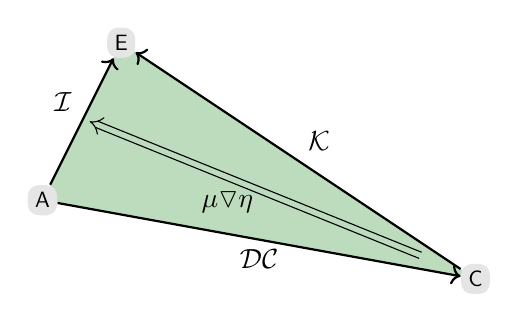
\begin{tikzpicture}
        \coordinate (t) at (0,0);
        \coordinate (b) at (-1,-2);
        \coordinate (d) at (1.75,-2.5); 
        \coordinate (c) at (4.5,-3); 
    
        \fill[color=ForestGreen!30] (t) -- (c) -- (b) -- cycle;
    
        \node[scale=0.8, rounded corners, fill=black!10] (Grp) at (t) {$\cat{E}$};
        \node[scale=0.8, rounded corners, fill=black!10] (G) at (b) {$\cat{A}$};
        \node[scale=0.8, rounded corners, fill=black!10] (H) at (c) {$\cat{C}$};
    
        \draw (G) edge[->, "{$\func{I}$}"{name=I, above left}, thick] (Grp);
        \draw (G) edge[->, "{$\func{DC}$}"{below}, thick] (H);
        \draw (H) edge[->, "{$\func{K}$}"{name=K, above right}, thick] (Grp);
    
        \draw[Rightarrow] (3.8,-2.7) -- (-0.4,-1) node[midway, below, yshift=2pt, xshift=-10pt] {$\mu\triangledown\eta$};
      \end{tikzpicture}
    };
  \end{tikzpicture}   

  \caption{The $\triangledown$-composition of counitals explains transitivity}
  \label{fig:compose-counitals}
\end{figure}  


\subsection{Categorifying isosceles counitals}
All extensions used in 
our proof of Theorem~\ref{thm:char-counital-eastern} 
lead to isosceles counitals. 
Counits---namely, counitals
$\fJ\fC\Rightarrow \fI$ in which $\fJ=\fI$ is 
the identity functor---are one
source of isosceles counitals. This hints at a way to characterize
characteristic subgroups.

We now prove that all counitals arising from characteristic subgroups extend to
isosceles counitals, thereby proving Theorem~\ref{thm:char-repn-eastern}. The most direct proof
might utilize \emph{Kan lifts}, the dual of the better known \emph{Kan
extensions}~\cite{Riehl}*{Chapter 6}, but we give a self-contained proof. 

Let $\fI:\cat{A}\to\cat{C}$ be an inclusion functor of categories and let
$\fC:\cat{A}\to \cat{C}$ be a functor. If $\counital : \fC \Rightarrow \func{I}$
is a natural transformation, then, for every object $X$ in $\acat{A}$, the
morphism $\counital_X : \func{C}(X) \to \func{I}(X)$ is a morphism in
$\acat{C}$. We consider the special case when this morphism is also in
$\acat{A}$.

\begin{defn}\label{def:internal-counital}
  A natural transformation $\counital:\fC \Rightarrow \func{I}$ is
  \emph{internal} if, for every object $X$ in $\cat{A}$, the
  morphism $\counital_X$ is a morphism in  $\acat{A}$.
\end{defn}



 



The property of being internal is strong. Take, for example, $\cat{A} =
\;\core{C}$, so the morphisms are exclusively isomorphisms. If $\counital$ is
internal, then $\iota_X : \func{C}(X) \to X$ is an isomorphism. Such an $\iota$
does not identify a new substructure.  In other words, $\cat{A}$ has too few
morphisms for our purposes. By extending the types of morphisms, we prove in
Proposition~\ref{prop:isosceles-to-internal} that every monic isosceles counital lifts to
an internal one, see~Figure~\ref{fig:extend-isosceles} for an illustration.


\begin{figure}[h]
  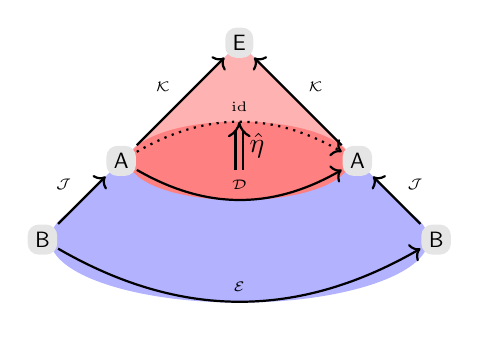
\begin{tikzpicture}[thick] 
    \coordinate (t) at (0,0);
    \coordinate (a) at (-1.5,-1.5);
    \coordinate (b) at (-2.5,-2.5);
    \coordinate (c) at ( 1.5,-1.5);
    \coordinate (d) at (2.5,-2.5);

    \fill[color=blue!30] (t) -- (b) -- (d) -- cycle;
    \fill[color=blue!30] (0,-2.5) ellipse (2.4cm and 0.8cm);
    \fill[color=red!30] (t) -- (a) -- (c) -- cycle;
    \fill[color=red!50] (0,-1.5) ellipse (1.4cm and 0.5cm);

    \node[scale=0.8, rounded corners, fill=black!10] (Grp) at (t) {$\cat{E}$};
    \node[scale=0.8, rounded corners, fill=black!10] (H) at (a) {$\cat{A}$};
    \node[scale=0.8, rounded corners, fill=black!10] (G) at (b) {$\cat{B}$};
    \node[scale=0.8, rounded corners, fill=black!10] (L) at (c) {$\cat{A}$};
    \node[scale=0.8, rounded corners, fill=black!10] (K) at (d) {$\cat{B}$};

    \draw (H) edge[->, "{\tiny $\func{K}$}"] (Grp);
    \draw (G) edge[->, "{\tiny $\func{J}$}"] (H);
    \draw (L) edge[->, "{\tiny $\func{K}$}"{above right}] (Grp);
    \draw (K) edge[->, "{\tiny $\func{J}$}"{above right}] (L);
    \draw (H) edge[->, out=30, in=150, dotted, "{\tiny $\id$}"{name=id}] (L);
    \draw (H) edge[->, out=-30, in=-150, "{\tiny $\func{D}$}"{name=D}] (L);
    \draw (G) edge[->, out=-30, in=-150, "{\tiny $\func{E}$}"] (K);

    \draw (D) edge[Rightarrow, "$\hat{\eta}$"{right}] (id);
  \end{tikzpicture}
  \caption{Extending an isosceles counital to an internal one}
  \label{fig:extend-isosceles}
\end{figure}


\pagebreak
\begin{prop}\label{prop:isosceles-to-internal}
  Let $\acat{E}$ be a category with subcategory $\acat{B}$ and inclusion
  $\func{I}$. Suppose  every object in $\acat{E}$ is also an object in
  $\acat{B}$. Let  $\eta : \func{I}\func{E} \Rightarrow \func{I}$ be a monic
  isosceles counital with $\func{E} : \cat{B} \to \cat{B}$. There exists a
  category $\acat{A}$ with inclusions $\func{J} : \acat{B}\to\acat{A}$ and
  $\func{K}:\acat{A}\to\acat{E}$, a functor $\func{D} : \acat{A}\to\acat{A}$,
  and an internal monic isosceles counital $\hat{\eta} : \func{K}\func{D}
  \Rightarrow \func{K}$ such that $\func{JE}=\func{DJ}$, $\func{I}=\func{KJ}$,
  and $\hat{\eta}\func{J} = \eta$.  
\end{prop}

 
\begin{proof}
  We define a subcategory $\cat{A}$ of $\cat{E}$ as follows: its objects are the
  objects of~$\acat{E}$; its morphisms are given as finite compositions of
  morphisms $\func{I}(\varphi):\acat{E}$, where $\varphi$ is a morphism in
  $\acat{B}$, and morphisms $\eta_X:\acat{E}$, where $X$ an object in
  $\acat{B}$. Hence, we have inclusions $\func{J} : \cat{B} \to \cat{A}$ and
  $\func{K} : \cat{A} \to \cat{E}$ such that $\func{I} = \func{KJ}$. Since both
  $\acat{A}$ and $\acat{B}$ have the same objects as $\acat{E}$, it follows that
  $\func{I}$, $\func{J}$, and $\func{K}$ are the identities on objects. Moreover, $\func{K}$ is the identity on morphisms.

  We now construct a functor $\fD:\cat{A}\to \cat{A}$ such that $\func{J}
  \func{E}= \fD \func{J}$. It suffices to define $\fD$ on morphisms and then
  verify that $\fD$ is a functor. Set
  \begin{align*} 
    \fD (\varphi) & = \begin{cases}
      \func{JE}(\varphi') & \varphi = \fJ(\varphi')\text{ for a morphism $\varphi'$ in } \cat{B}, \\
      \eta_{\func{E}(X)} & \varphi=\eta_X\text{ for some object $X$ in $\acat{B}$}, \\
      \func{D}(\sigma)\func{D}(\tau) & \varphi=\sigma\tau.
    \end{cases}
  \end{align*}
  If $\fD$ is well defined, then $\func{D}(\varphi)$ is a morphism in
  $\acat{A}$, and $\func{J} \func{E}=\fD \func{J}$ by construction. To verify
  that $\fD$ is well defined, it suffices to consider the case where  $\eta_X$
  (with $X$ an object in $\acat{B}$) is also a morphism in $\acat{B}$:
  specifically, there is a morphism $\beta :\acat{B}$ such that $\eta_X =
  \func{I}(\beta)$. Since $\fI$ is the identity on objects, $\beta : \fE(X) \to
  X$. We will show that $\eta_{\func{E}(X)}=\fK\fD(\eta_X)=\func{IE}(\beta)$. To
  see this, we apply $\eta$ to the morphism $\beta:\func{E}(X)\to X$ and obtain
  the following diagram (see shaded entry $(2,2)$ of
  Figure~\ref{fig:functor-cat-act}).
  \[ 
    \begin{tikzcd}
      \func{I}\func{E}\func{E}(X) \arrow[r, "\func{IE}(\beta)"] \arrow[d, "\eta_{\fE(X)}"] 
        & \func{I}\func{E}(X) \arrow[d, "\eta_{X}"] \\
      \func{I}\func{E}(X) \arrow[r, "\func{I}(\beta)"] & \func{I}(X)
    \end{tikzcd}
  \]
  Since $\eta_X = \fI(\beta)$, the diagram implies that $\eta_X
  \eta_{\func{E}(X)}=\eta_X \func{IE}(\beta)$. Since $\eta_X$ is monic by
  assumption,  $\func{IE}(\beta)=\eta_{\func{E}(X)}$. This proves that
  $\func{D}$ is well defined. 

  We claim that there exists a natural transformation
  $\hat{\eta}:\func{K}\func{D}\Rightarrow \func{K}$ such that
  $\hat{\eta}\func{J} = \eta$. 
  Since the
  objects of $\cat{A}$ are those of $\cat{B}$, we define $\hat{\eta}_X$ to be
  $\eta_X$ and show that this yields the required counital. First, we consider
  the case that $\varphi : X\to Y$ is a morphism in $\cat{B}$. Then $\func{K} \func{D}
  \func{J}(\varphi)=\func{K} \func{J} \func{E}(\varphi)=\func{I}
  \func{E}(\varphi)$, so
  \begin{align*}
    \hat{\eta}_Y \func{K} \func{D}(\func{J}(\varphi)) 
    & = \eta_Y \func{I} \func{E}(\varphi) = \func{I}(\varphi)\eta_X 
     = \func{K}(\func{J}(\varphi))\hat{\eta}_X.
  \end{align*} 
  Now we assume $\varphi = \eta_X: \func{IE}(X)\to \func{I}(X)$ for some
  object $X$ in $\cat{B}$. Since $\fI$ is the identity on objects and $\fK$ is the identity on morphisms, 
  \begin{align*}
    \hat{\eta}_{\func{I}(X)} \func{K} \func{D}(\eta_X) 
    & = \hat{\eta}_X\func{KD}(\eta_X) = \eta_{X} \func{K}(\eta_{ \func{E}(X)})  
     = \eta_{X} \eta_{ \func{E}(X)}  = \func{K}(\eta_X)\hat{\eta}_{ \func{E}(X)}.
  \end{align*}
  Lastly, we consider the case of an arbitrary finite composition
  $\varphi=\varphi_1\cdots \varphi_n$ where each  $\varphi_k$ is either $\fJ(\varphi_k')$ for some morphism $\varphi_k'$ in $\acat{B}$ or a morphism $\eta_X$ for some object $X$ in $\acat{B}$. It suffices to consider
  only the case where $n=2$, say $\varphi = \varphi_1\varphi_2$ with $\varphi_2
  : X\to Z$ and $\varphi_1: Z\to Y$. Now 
  \begin{align*}
    \hat{\eta}_Y \func{K} \func{D}(\varphi) 
    & = \hat{\eta}_Y \func{K} \func{D}(\varphi_1) \func{K} \func{D}(\varphi_2) \\
    & = \func{K}(\varphi_1)\hat{\eta}_{Z} \func{K} \fD(\varphi_2) \\
    & = \func{K}(\varphi_1) \func{K}(\varphi_2)\hat{\eta}_{X}\\
    & = \func{K}(\varphi)\hat{\eta}_X.
  \end{align*} 
 Thus, 
$\hat{\eta}:\func{K} \func{D}\Rightarrow \func{K}$. Since $\eta$ is monic, so is $\hat{\eta}$.  Also, $\hat{\eta}_X$ is a morphism in $\cat{A}$ for every object $X$, so it is  internal, as claimed.
\end{proof}





We now prove that every characteristic substructure of an eastern
algebra is induced by a morphism of category biactions.

\begin{thm}\label{thm:char-from-biacts}
  Let $X$ be an object in a category $\cat{E}$ of eastern algebras. Let $Y$ be characteristic in $X$ with inclusion $\iota: Y\to X$. There
  exist subcategories $\cat{A}$ and $\cat{B}$ with $\core{E}\leq \cat{A},\cat{B}\leq \cat{E}$, and an $(\acat{A},\acat{B})$-morphism $\func{M} : \acat{B}
  \to \acat{A}$ such that $\func{M}(\id_X\cdot \one_{\acat{B}}) = \iota$.
\end{thm} 

\begin{proof}
Let $\func{I}: \core{E}\to \acat{E}$ be  the inclusion functor. The proof of
  Theorem~\ref{thm:char-counital-eastern} shows that there exists  a functor
  $\func{E}:\;\core{E}\;\to \;\core{E}$ and a monic counital $\eta:\func{I}
  \func{E}\Rightarrow \func{I}$ such that  $\eta_X=\iota$. We use
  Proposition~\ref{prop:isosceles-to-internal}  (with $\cB=\;\core{E}$) to create
  a category $\cat{A}$ generated from $\core{E}$ and $\eta$, an inclusion
  functor $\func{K} : \cat{A} \to \cat{E}$, a functor $\func{D} : \cat{A} \to
  \cat{A}$, and an internal monic counital $\hat{\eta} : \func{K}\func{D}
  \Rightarrow \func{K}$ with  $\hat{\eta}_{Z}=\eta_Z$ for all objects in
  $\core{E}$. Lastly, we  apply Proposition~\ref{prop:nat-trans-biact}(a) to
  $\hat{\eta}$ to obtain an $\acat{A}$-bimorphism $\mathcal{N} : \acat{A} \to
  \acat{E}$ such that $\hat{\eta} = \mathcal{N}(\one_{\acat{A}})$. Since
  $\hat{\eta}$ is internal, there exists an $\acat{A}$-bimorphism $\mathcal{M} :
  \acat{A} \to \acat{A}$ such that $\mathcal{N}=\mathcal{KM}$. Hence,
  $\hat{\eta}=\func{K}\func{M}(\one_{\acat{A}})$. With $\acat{B} \defeq
  \acat{A}$, it follows that  $\mathcal{M}(\id_X\cdot \one_{\acat{B}})
  =\hat{\eta}_X=\eta_X=\iota$, as claimed.
\end{proof}

\subsection{Proofs of main theorems}\label{sec:proofs} Having developed the
required theory, we can now complete the proofs of our main results.
Theorem~\ref{thm:char-counital} is a special case of
Theorem~\ref{thm:char-counital-eastern}, which we proved 
in the previous section.

\medskip 

\noindent\textit{Proof of Theorem} \ref{thm:char-repn-eastern}.
If (1) holds, then Theorem~\ref{thm:char-from-biacts} yields (3). 
If (3) holds, then (2) follows from Theorem~\ref{thm:counit-capsules}\ref{thmpart:bicap-to-counit}  and the fact that 
$\iota=\mathcal{M}(\id_G\cdot\one_{\cat{B}})$. If (2) holds, then (1) follows from 
Theorem~\ref{thm:char-counital-eastern}. \qed  

\medskip
\noindent
Theorem~\ref{thm:char-repn} follows from 
Theorem~\ref{thm:char-repn-eastern}.


\subsection{Duality} 
\label{sec_dual} 
 Recall from  Section~\ref{sec:proofThm1} that a natural
transformation $\eta : \func{I} \Rightarrow \func{D}$ is a unital if  $\func{I}$ is an
inclusion functor. If $\func{I} = \id$, then $\eta : \id
\Rightarrow \func{D}$ is a \emph{unit}. A unital $\eta : \func{I} \Rightarrow
\func{D}$ is \emph{epic} if $\eta_X : \func{I}(X) \to \func{D}(X)$ is
epic for all objects $X$. Units and unitals are the duals 
of counits and counitals. 


We state a dual analogue of Theorem~\ref{thm:char-repn-eastern} for characteristic quotients in
eastern algebras; its proof follows \emph{mutatis mutandis} from that 
of Theorem~\ref{thm:char-repn-eastern}.


\begingroup     
\renewcommand{\themainthm}{2-dual} 
\begin{mainthm}\label{thm:general-dual}
  Let $\acat{E}$ be an eastern variety, and let $G$ be an object of
  $\acat{E}$ with quotient $Q$ and projection $\pi$. There exist categories
  $\acat{A}$ and $\acat{B}$, where $\core{E}\; \leq \acat{A} \leq \acat{E}$,
  such that the following are equivalent.
  \begin{ithm}
    \item[\rm (1)] $Q$ is a characteristic quotient of $G$.
    \item[\rm (2)] There is a functor $\func{U} : \acat{A} \to \acat{A}$ and a unit
    $\epsilon : \id_{\acat{A}} \Rightarrow \func{U}$ such that $Q =
    \mathrm{Coim}(\epsilon_{G})$.
    \item[\rm (3)] There is an $(\acat{A},\acat{B})$-morphism $\func{M} : \acat{A} \to
    \acat{B}$ such that $\pi = \func{M}(\one_{\acat{A}}\cdot \id_G)$.
  \end{ithm}
\end{mainthm}
\endgroup


Although a characteristic subgroup of a group $G$ is associated with a
characteristic quotient of $G$, and vice-versa, there are subtle differences in
other categories of eastern algebras. 

\begin{ex}\label{ex:unital-rings}
  Let $\mathbb{Q}$ be the ring of rational numbers and $\mathbb{Z}$ its subring
  of integers. If $\varphi : \mathbb{Q}\to\mathbb{Q}$ is a homomorphism of
  unital rings, then $\varphi(1)=1$. This forces $\varphi=\id_\mathbb{Q}$, so
  $\mathbb{Z}$ is fully invariant in $\mathbb{Q}$. Since $\mathbb{Q}$ is a
  field, its only quotients are itself and the trivial ring. Hence, $\mathbb{Q}$
  has many fully-invariant substructures, but only two fully-invariant
  quotients.
  \exqed 
\end{ex} 

In general, kernels of group homomorphisms are representable as subgroups
(unlike ideals, which are not necessarily unital subrings). Conversely, every
characteristic subgroup is normal and has an associated quotient. Formalizing
these observations, we say that 
invariant structures of groups are
\emph{self-dual} up to equivalence of natural transformations in $\cat{Cat}$,
see \cite{HoTT}*{pp.~59--61}.   The next proposition provides a categorical
description of this observation for $\cat{Grp}$; we use it in 
Section \ref{sec:examples}.

\begin{prop}\label{prop:kernel}
  The following hold for categories 
  $\lcore{Grp}\;\leq \cat{A}\leq \cat{Grp}$ and $\cat{B}\leq \cat{Grp}$
  with inclusion functors $\func{I}:\acat{A} \to \acat{Grp}$ and
  $\func{J}:\acat{B}\to \acat{Grp}$.
  \begin{ithm} 
    \item Given a unital $\unital:\func{I}\Rightarrow \func{J}\func{U}$, there
    is a category $\cat{C}\leq \cat{Grp}$, with inclusion $\func{K}$, and a
    functor $\func{C} : \cat{A} \to \cat{C}$ such that $\ker(\unital) :
    \func{K}\func{C}\Rightarrow \func{I}$ is a counital where $\func{C}(G) = \ker(\unital_G)$ and $(\ker (\unital))_G
    : \ker(\unital_G)\hookrightarrow G$ is the inclusion for every group $G$.

    \item Given a counital $\counital:\func{J}\func{C}\Rightarrow \func{I}$,
    there is a category $\cat{C}\leq \cat{Grp}$, with inclusion 
    $\func{K}$, and a functor $\func{U} :
    \cat{A}\to \cat{C}$ such that $\coker (\counital): \func{I}\Rightarrow
    \func{K} \func{U}$ is a unital where $\func{U}(G)=G/\im (\counital_G)$ and $(\coker (\counital))_G : G \twoheadrightarrow G/\im (\counital_G)$ for every group $G$.


    \item With the notation of {\rm (a)} and {\rm (b)},  there are unique invertible 
    $\mu,\tau:\cA$ such that   $\coker (\ker (\unital))=\mu (\mathrm{im}(\pi))$ and 
    $\ker
    (\coker (\counital))= \counital\tau$.
  \end{ithm}
\end{prop}

\begin{proof}
  \begin{iprf}
  \item For every morphism $\varphi:G\to H$ in $\cat{A}$, there is an induced
  morphism $\varphi':\im(\unital_G)\to \im (\unital_{H})$ such that
  $\varphi'\unital_{G}=\unital_H\varphi$, so
  \[
    \unital_{H}\varphi(\ker(\unital_G))
    =\varphi' \unital_G (\ker (\unital_G))=1.
  \]
  Therefore $\varphi(\ker(\unital_G))\leq \ker (\unital_{H})$.
  In particular, the restriction 
  \begin{equation*}
    \varphi|_{\ker (\unital_G)}:\ker(\unital_G)\to \ker(\unital_{H})
  \end{equation*}
  is well defined. Let $\cat{C}$ be the category whose objects
  are $\ker(\unital_G)$ for all groups $G$ and whose morphisms are $\varphi|_{\ker (\unital_G)}$ for all morphisms $\varphi : G\to  H$ in $\cat{A}$. Let $\func{K}: \acat{C}\to \acat{Grp}$ be the inclusion functor. Moreover,
  there is a functor $\func{C}: \cat{A} \to \cat{C}$ given
  by $\func{C}(G) = \ker(\unital_G)$ and $\func{C}(\varphi) = \varphi|_{\ker
  (\unital_G)}$. If we define $\counital_G: \ker(\unital_G)\hookrightarrow G$ to be the
  associated inclusion map for the kernel, then  $\counital:
  \func{K}\func{C}\Rightarrow \func{I}$ is the required counital.

  \item The proof is dual to that of (a).

  \item Consider the unital $\unital : \func{I} \Rightarrow
  \func{J} \func{U}$. By Theorem~\ref{thm:Noether},
  for each group $G$ there is an isomorphism
  \[ 
    \mu: \fU(G)=\mathrm{Im}\pi_G \to  G/\ker\unital_G=\coker (\ker\unital_G).
  \] 
  Thus, 
$\coker (\ker (\unital))=\mu (\text{im}(\pi))$; 
   likewise, for $\ker (\coker (\counital))$ and  $\counital$. \qedhere
  \end{iprf}
\end{proof}


\section{Categorification of standard characteristic subgroups}
\label{sec:examples}

Theorem~\ref{thm:char-repn} states that every characteristic subgroup can be studied in
three ways: as a group, as a natural transformation, and as a morphism of category
biactions. In this section, we describe common characteristic subgroups using  
all three forms. In so doing, we reveal insights gained from the categorical perspective. 

Throughout, we use the following notation for restriction and induction. Let $\varphi : G \to H$ be a homomorphism of groups, and let
$\func{C}(G)$ and $\func{C}(H)$ be subgroups of $H$ and $G$, respectively. 
If the restriction of $\varphi$ to $\func{C}(G)$ maps into $\func{C}(H)$, 
then we denote it by 
\begin{align}\label{eqn:restriction} 
  \varphi|_{\func{C}} : \func{C}(G) \to \func{C}(H),\quad c\mapsto \varphi(c).
\end{align} 
Similarly, if $\varphi$ maps a normal subgroup  $\func{Q}(G)$ of $G$ into a normal subgroup $\func{Q}(H)$ of $H$, then the \emph{induction} of $\varphi$ via $\func{Q}$ is
\begin{align}\label{eqn:induction}
  \varphi|^{\func{Q}} : G/\func{Q}(G) \to H/\func{Q}(H),\quad g\func{Q}(G) \mapsto \varphi(g)\func{Q}(H).
\end{align}
  

\subsection{Abelianization and derived subgroups}\label{sec:abelianization}

Figure~\ref{fig:comm} gives the three perspectives on the derived subgroup. We
develop this example, so that we may also treat the lower central series 
and all verbal subgroups in Section~\ref{sec:lower-central}.

The counital $\lambda : \func{D}\Rightarrow \id_{\cat{Grp}}$ 
of Example~\ref{ex:three-chars}
associated with the derived subgroup $\gamma_2(G)$ of a group $G$ 
can be constructed also as the kernel of the unital 
associated with abelianization.
We explore the category biaction interpretation.
Let $\acat{Abel}$ be the category of abelian groups, a subcategory of
$\cat{Grp}$ with inclusion $\func{I} : \acat{Abel} \to \acat{Grp}$. We define a
morphism $\func{A} : \cat{Grp} \to \cat{Abel}$ given by $\varphi\mapsto
\varphi|^{\gamma_2}$. The functors $\func{A}$ and
$\func{I}$ turn the categories $\acat{Grp}$ and $\acat{Abel}$ into $(\acat{Grp},
\acat{Abel})$-bicapsules. 

We show that $\func{A}:\acat{Grp}\to\acat{Abel}$ is a $(\acat{Grp},
\acat{Abel})$-morphism. Let $\varphi$ and $\tau$ be group homomorphisms, and
let $\alpha$ be a homomorphism of abelian groups. Now 
\begin{align*}
  \func{A}(\alpha\cdot \varphi\tau) &= (\func{I}(\alpha)\varphi\tau)|^{\gamma_2} = \alpha\;\varphi|^{\gamma_2}\;  \tau|^{\gamma_2} =\alpha\func{A}(\varphi)\cdot \tau.
\end{align*}
To obtain the counital associated with the derived subgroup, we apply
Proposition~\ref{prop:kernel} and take the kernel of $\func{A}(\one_{\acat{Grp}})$. Since
the unital-counital pair obtained through this process is a unit-counit pair, 
 we
obtain the well-known observation that the derived subgroup is fully invariant.

\begin{figure}[h]
  \centering
  \includegraphics[width=\textwidth]{graphics/commutator.pdf}
  \caption{Three perspectives on the derived subgroup}
  \label{fig:comm}
\end{figure}


\subsection{Verbal subgroups}
\label{sec:lower-central}

We generalize the approach taken in Section~\ref{sec:abelianization}. Let $\Omega$ be
the group signature from~Example~\ref{ex:group-grammar}. To each set $W$ of words from
the free group $\Omega\langle X\rangle$ we associate a category $\acat{Var}(W)$ as follows (see Section~\ref{sec:free}). 
For each word $w :W$, group
$G$, and $X$-tuple $g\tin G^X$, define $w_G : G^X \to G$ by $g\mapsto \mathrm{eval}_g(w)$. 
Define $\acat{Var}(W)$ to be the full subcategory of $\cat{Grp}$
with objects 
\[
  \{ G:\cat{Grp} \mid (\forall g\tin G^X) (\forall w\tin W)\; w_G(g)=1\}
\]
with inclusion functor $\func{I}:\acat{Var}(W)\to \cat{Grp}$. The category
$\acat{Var}(W)$ is the \textit{group variety} with laws $W$. Let $\mathrm{Rad}_W(G)$ be the minimal normal subgroup of a group $G$ such that $G/\mathrm{Rad}_W(G)$ is in $\mathsf{Var}(W)$. Let
$\func{R}:\cat{Grp}\to \acat{Var}(W)$ be the functor such that $\func{R}(G)$ is the
largest quotient of $G$ contained in $\acat{Var}(W)$, where the functor carries $G$ 
to $G/\mathrm{Rad}_W(G)$, and morphisms $\varphi$ are sent to $\varphi|^{\mathrm{Rad}_W}$. 

\begin{prop}\label{prop:verbal}
The functors $\func{R}$ and $\func{I}$ form an adjoint functor pair: 
  $\func{R} : \acat{Grp}\dashv \acat{Var}(W) : \func{I}$.
\end{prop}

\begin{proof}
  By Proposition~\ref{prop:functors-are}, the functors $\func{R}$ and $\func{I}$ turn both
  $\acat{Var}(W)$ and $\acat{Grp}$ into $(\acat{Var}(W),\acat{Grp})$-bicapsules. The
  functor $\func{R}$ is a $(\acat{Var}(W),\acat{Grp})$-morphism: for morphisms
  $\alpha$ in $\acat{Var}(W)$ and $\varphi,\tau$ in $\acat{Grp}$, 
  \begin{align*}
    \func{R}(\alpha\varphi\cdot\tau) &= (\alpha\varphi\func{I}(\tau))|^{\mathrm{Rad}_W} = \alpha|^{\mathrm{Rad}_W}\; \varphi|^{\mathrm{Rad}_W}\; \tau = \alpha\cdot \func{R}(\varphi)\tau.
  \end{align*}
  Since $\func{R}$ and $\func{I}$ are pseudo-inverses,
  the result follows from Theorem~\ref{thm:iso-biacts-adjoints}\ref{thmpart:biaction-to-adjoint}. 
\end{proof}

The adjoint functor pair in Proposition~\ref{prop:verbal} categorifies verbal subgroups.
The dual version of Theorem~\ref{thm:counit-capsules} describes how to obtain the
unit $\pi : \id_{\acat{Grp}}\Rightarrow \func{IR}$ from~$\func{R}$. Applying
Proposition~\ref{prop:kernel}, the kernel of $\pi$ yields a counit $\iota : \func{V}
\Rightarrow \id_{\acat{Grp}}$ for some functor $\func{V}: \acat{Grp} \to
\acat{Grp}$. If $G$ is a group, then  $\func{V}(G)$ is the \emph{$W$-verbal} subgroup.
We conclude that all verbal subgroups are fully invariant.
Thus, from Proposition~\ref{prop:verbal}, we get an \emph{exact sequence} of natural
transformations
\begin{center}
\begin{tikzcd}
  \func{V} \arrow[r,Rightarrow,"\ker(\pi)"] & \id_{\cat{Grp}} 
  \arrow[r,Rightarrow,"\unital"] & \func{IR}.
\end{tikzcd}
\end{center} 
The corresponding diagram appears in Figure~\ref{fig:verb-W}.


\begin{figure}[h]
  \centering
  \includegraphics[width=\textwidth]{graphics/verbal.pdf}
  \caption{Three perspectives on verbal subgroups}
  \label{fig:verb-W} 
\end{figure}


\subsection{Marginal subgroups}
\label{sec:center}

Now we consider characteristic subgroups such as the center $\zeta(G)$ of a
group $G$.  As seen in Example~\ref{ex:three-chars_first},  there are group homomorphisms 
$\varphi:G\to H$ for which $\varphi(\zeta(G))\not\leq \zeta (H)$, so,
unlike verbal subgroups, the center is not fully invariant. This fact is
revealed by the categorification of the center---it does not yield a counit
between functors $\acat{Grp}\to \acat{Grp}$, but rather a proper counital between functors of
the form $\lepi{Grp}\; \to\acat{Grp}$, where $\lepi{Grp}$ is the category of
groups whose morphisms are epimorphisms. We establish this fact more generally
for the class of \textit{marginal subgroups} introduced by P.\ Hall
\cite{Hall40}.

\begin{ex}[Hall's Isoclinism]\label{ex:isoclinism}
 For an integer $n>0$ we write $G^n$ for the $n$-fold direct product 
of a group $G$. 
  The commutator map $\kappa:G^2 \to G$ 
is given by $(g,h) \mapsto [g,h]\defeq g^{-1}h^{-1}gh$.
We define a congruence relation
  $\equiv$ on $G$ and write $x\equiv z$ if and only if $[x,z]=[y,z]$ for all $y: G$.
Factoring through
  this congruence relation and restricting the outputs to the verbal subgroups,
  we obtain a 
map $*:(G/\zeta(G))^2\to \gamma_2(G)$ such that the following diagram commutes.
  \begin{equation*} 
    \begin{tikzcd}
      G^2\arrow[r,"{\kappa}"]\arrow[d,two heads] & G\\
      (G/\zeta(G))^2\arrow[r,"*"] & {\gamma_2(G)}\arrow[u,hook]
    \end{tikzcd}
  \end{equation*}  
  Two groups are \emph{isoclinic} if their 
commutator maps are equivalent.~\exqed
\end{ex}


For each group $G$ and each word $w$, there is a unique minimal normal subgroup $w^*(G)$ such that the
  map $\overline{w}_G : (G/w^*(G))^n \to G$ given by 
  \begin{align*}
    (g_1w^*(G),\dots, g_nw^*(G)) &\longmapsto w_G(g_1,\dots, g_n)
  \end{align*}
  is non-degenerate: namely,
fixing any $n-1$ entries of the $n$-tuple argument of 
$\overline{w}_G$ yields an injective map $G/w^*(G) \to G$. 
Here $w_G$ is as defined in Section~\ref{sec:lower-central}.

For a set $W$ of words, the associated \emph{marginal subgroup} of a group $G$ is defined as  $W^*(G)=\bigcap_{w:W} w^*(G)$. Clearly, $W^*(G)$ is characteristic in $G$. The image
of $\overline{w}_G$, and thus also $w_G$, is the verbal subgroup associated with
$w$, written $w(G)$. 
\begin{figure}[!tbp] 
  \centering
  \includegraphics{graphics/center-story.pdf}
  \caption{Marginal subgroups and quotients categorified}
  \label{fig:log-W-star} 
\end{figure}

Hall \cite{Hall40}
introduced the general notion of \emph{isologism} for word-map
equivalence. We extend this language to categories.
Each word $w$ determines a category $\lepi{Log}_{w}$ with maps
$\overline{w}_G : (G/w^*(G))^n\to w(G)$ as objects, where the 
morphisms are pairs
$(\varphi_1,\varphi_2)$ of group epimorphisms such that the following diagram
commutes.
\begin{center}
  \begin{tikzcd}
    (G/w^*(G))^n\arrow[r, "\overline{w}_G"]\arrow[d, "\varphi_1^n"] & w(G) \arrow[d, "\varphi_2"] \\ 
    (H/w^*(H))^n \arrow[r, "\overline{w}_H"] & w(H)
  \end{tikzcd}
\end{center}
We define two functors. The first is $\func{L} : \;\lepi{Grp}\; \to \;\lepi{Log}_w$
given by $G\mapsto \overline{w}_G$ and $\varphi\mapsto (\varphi|^{w^*},
\varphi|_w)$. The second is $\func{P}:\;\lepi{Log}_w\;\to \;\lepi{Grp}$ given by
$\overline{w}_G\mapsto G/w^*(G)$ and $(\varphi_1,\varphi_2)\mapsto \varphi_1$.
For a group $G$, let $\pi_G : G \twoheadrightarrow G/w^*(G)$ be the usual projection homomorphism. 
Now $\pi :
\id_{\lepi{Grp}}\Rightarrow \func{PL}$ is a unit. Let $\func{I} :
\;\lepi{Grp}\; \to \acat{Grp}$ be the inclusion functor.
Then the unital $\func{I}\pi : \func{I}\Rightarrow
\func{IPL}$ is a categorification of marginal quotients.

To categorify the marginal
subgroup, we take the kernel of $\pi$ via Proposition~\ref{prop:kernel} and compose with
$\func{I}$: namely, $\func{I}\ker(\pi) : \func{IC}\Rightarrow \func{I}$ for some
functor $\func{C} : \;\lepi{Grp}\; \to \;\lepi{Grp}$. Figure~\ref{fig:log-W-star}
displays the various morphisms and their relationships. This
construction demonstrates that  marginal subgroups are not just
characteristic, but invariant under all epimorphisms.

The construction applies to other algebraic structures by simply involving
formulas in the appropriate signature. However, the notion of congruence does
not always yield a substructure, so the structures are 
more naturally expressed as characteristic quotients.

\section{Composite characteristic structures}
\label{sec:compose}
We now address one remaining powerful feature of our categorical description of characteristic 
structure. It relates to a comment we made 
after Theorem~\ref{thm:char-repn}:  a characteristic subgroup  may 
arise from $(\acat{A},\acat{B})$-morphisms $\acat{B}\to\acat{A}$
where $\acat{B}$ is \textit{not} a category of groups. 
We give one illustration of how this ``transferability'' 
explains techniques currently used in isomorphism tests. 

In~\cite{Wilson:filters}*{\S 4}, it is shown that
a $p$-group $G$ of class at most $2$ with exponent $p$ has a 
characteristic subgroup induced by the Jacobson radical of an 
algebra associated to the bilinear commutator map of $G$. 
Here we construct that characteristic subgroup using a tensor 
product of capsules, as described in~Section~\ref{sec:ext-prob}.

\subsection{From groups to bimaps}\label{sec:delta}

Fix an odd prime $p$, and let  $\cat{G}\defeq \lcore{Grp}_{2,p}$ be the category
whose objects are $p$-groups of class at most $2$ with exponent $p$, and whose
morphisms are isomorphisms. The objects of $\cat{G}$ are groups $G$ with
exponent $p$ and central derived subgroup, so $\gamma_2(G)\leq \zeta(G)$. 

Let $\mathbb{F}_p$ be the field with $p$ elements, and let 
$\cat{B}\defeq \lcore{Bi}(\mathbb{F}_p)$ be the category of alternating $\mathbb{F}_p$-bilinear maps. 
The objects of $\cat{B}$ are bilinear maps $b: V\times V\to W$, 
where $V$ and $W$ are $\mathbb{F}_p$-spaces, such that $b(u,v)=-b(v,u)$ 
for all vectors $u,v$. For
objects $b : V\times V \to W$ and $b' : V'\times V' \to W'$ in $\acat{B}$, 
a morphism $\varphi : b \to b'$ is a pair of invertible linear maps 
$(\alpha : V\to V', \beta: W\to W')$ such that,
 for all $u,v\in V$,
\begin{equation*}
     b'(\alpha u, \alpha v)  = \beta b(u,v).
\end{equation*}

Define a functor  
$\func{B} : \cG\to \cB$ that takes a group $G$ to 
\[
    b_G: G/\gamma_2(G) \times G/\gamma_2(G) \to \gamma_2(G),
    \quad (x\gamma_2(G),y\gamma_2(G))\mapsto [x,y],
\]
and a homomorphism $\varphi : G\to H$ to the pair $(\varphi|^{\gamma_2},\
\varphi|_{\gamma_2})$, as defined in \eqref{eqn:restriction} and
\eqref{eqn:induction}. Since $G$ has exponent $p$ and $\gamma_2(G)\leq \zeta(G)$
by assumption,  
$b_G$ is an alternating $\mathbb{F}_p$-bilinear map.

Next, define a functor $\func{G} : \cB \to \cG$
that takes an $\mathbb{F}_p$-bilinear map
$b : V\times V\to W$ to the group $G_b$ on
$V\times W$ with binary operation
\[
    (v_1,w_1) \cdot (v_2,w_2) = \left(v_1+v_2, w_1+w_2 + \frac{1}{2}b(v_1,v_2)\right).
\] 
A morphism $(\alpha, \beta)$ from $b:V\times V\to W$ to $b':V'\times V'\to W'$ 
in $\cat{B}$ induces a group isomorphism, denoted $\alpha\boxtimes \beta$,
mapping $G_b=V\times W$ to $G_{b'}=V'\times W'$
by
\begin{equation*}
    (\alpha\boxtimes \beta)(v,w) \defeq (\alpha u, \beta w). 
\end{equation*}


\begin{lem}
    \label{lem:Baer}
    The functor $\func{B}:\cG\to \cB$ is  
    a $(\cG,\cB)$-morphism.
\end{lem}

\begin{proof}
    The functor $\func{B}$ induces a left $\acat{G}$-action on (the morphisms of) 
    $\cB$,
    and $\func{G}$ induces a right $\acat{B}$-action on $\cG$,
    so $\cB$ and
    $\cG$ are $(\cB,\cG)$-bicapsules.
    Let $\lambda, \mu$ be morphisms of $\cG$ and let $(\alpha,\beta)$ be a
    morphism of $\cB$ such that $\lambda \mu\cdot (\alpha,\beta) =
    \lambda\mu (\alpha\boxtimes \beta)$ is defined.
     Now
    \begin{align*}
        \func{B}(\lambda\mu\cdot (\alpha,\beta)) 
        &= \left((\lambda\mu(\alpha\boxtimes\beta))|^{\gamma_2},\ (\lambda\mu(\alpha\boxtimes\beta))|_{\gamma_2}\right) \\
        &= \left(\lambda|^{\gamma_2} \mu|^{\gamma_2}\alpha,\ \lambda|_{\gamma_2} \mu|_{\gamma_2} \beta\right) \\ &= \lambda \cdot\func{B}(\mu) (\alpha,\beta),
    \end{align*}
    so $\func{B}$ is a $(\cG,\cB)$-morphism. 
\end{proof}

By applying the dual version of Theorem~\ref{thm:counit-capsules}\ref{thmpart:bicap-to-counit},
    we obtain a unit $\id_{\cG}\Rightarrow \func{BG}$.  
    There is also a 
    counit 
    $\id_{\cG}\Leftarrow \func{BG}$. Together
    these give a categorical interpretation 
    of the {\it Baer correspondence}~\cite{Baer}.

\subsection{From bimaps to algebras}
\label{sec:gamma}
Let $\cA\defeq \lcore{Alge}(\mathbb{F}_p)$ be the category of $\mathbb{F}_p$-matrix algebras with 
algebra isomorphisms.  Using \cite{Wilson:filters}*{\S 4}, define a functor 
$\func{A}:\cB\to \cA$ by
\begin{align*} 
    \func{A}(b)&= \left\{f \in \End(V)
    ~\middle|~ \exists f^*\in\End(V)^{op},\forall u,v \in V,\; b(fu, v) = b(u, f^*v) \right\}.
\end{align*}
Invertible morphisms $(\alpha,\beta)$ in $\cB$ from 
$b:V\times V\to W$ to $b':V'\times V'\to W'$ are  sent to 
\begin{equation*}
    \func{A}(\alpha,\beta):
    f\in \func{A}(b) \mapsto f^{\alpha^{-1}}\in \func{A}(b').
\end{equation*}
  
\begin{fact}
\label{fact:adj-ten}
    The functor $\func{A}$ is a $(\cB,\cA)$-morphism.
\end{fact}

\subsection{From matrix algebras to semisimple algebras}
\label{sec:upsilon}
Every matrix algebra $A$ over a field is Artinian, so 
the quotient 
of $A$ by its Jacobson radical $\mathrm{Jac}(A)$ 
is a semisimple algebra. The map 
$A\mapsto A/\mathrm{Jac}(A)$ is 
a functor from $\acat{A}$ to the 
category $\cS\defeq \lcore{SSAlge}(\mathbb{F}_p)$ of 
semisimple $\mathbb{F}_p$-algebras. It is also an 
$(\cA,\cS)$-morphism.

\subsection{Combining capsules}

Recall that 
\begin{align*}
\cat{G}= \lcore{Grp}_{2,p}, \qquad \cat{B}= \lcore{Bi}(\mathbb{F}_p), \qquad
\cat{A}= \lcore{Alge}(\mathbb{F}_p), \qquad \cat{S}= \lcore{SSAlge}(\mathbb{F}_p).
\end{align*}
Denote by $\Delta$ the bicapsule associated to the $(\cG,\cB)$-morphism in Lemma~\ref{lem:Baer}.
Denote by $\Gamma$ and $\Upsilon$, respectively, the bicapsules associated to the 
$(\cB,\cA)$- and $(\cA,\cS)$-morphisms in Fact~\ref{fact:adj-ten} and Section~\ref{sec:upsilon}. 
These three capsules can now be combined to 
produce the $(\cG,\cS)$-capsule
\begin{align*}
    \Delta \otimes_{\cat{B}} \Gamma \otimes_{\cat{A}} \Upsilon
    = \cat{G}\cdot \mu\cdot  \cat{S}.
\end{align*}
The resulting generator $\mu$ of this cyclic bicapsule is  
a unital. By Theorem~\ref{thm:general-dual} this provides the 
characteristic subgroup used in \cite{Maglione:adjoints} and \cite{Wilson:filters}*{\S 4}.

 


\section*{Acknowledgements}
We thank Chris Liu for fruitful discussions and some proof-of-concept
implementations.  We thank John Power and 
Mima Stanojkovski for comments on a draft. 
Brooksbank was supported by NSF grant DMS-2319371. 
Maglione was supported by DFG grant VO 1248/4-1 (project
number 373111162) and DFG-GRK 2297. 
O’Brien was supported by the Marsden Fund of New Zealand Grant 23-UOA-080
and by a Research Award of the Alexander von Humboldt Foundation.
Wilson was supported by a Simons Foundation Grant
identifier \#636189 and by NSF grant DMS-2319370.

\begin{bibdiv}
\begin{biblist}

\bib{AR1994:categories}{book}{
	author={Ad\'{a}mek, Ji\v{r}\'{\i}},
	author={Rosick\'{y}, Ji\v{r}\'{\i}},
	title={Locally presentable and accessible categories},
	series={London Mathematical Soc.\ Lecture Note Ser.},
	volume={189},
	publisher={Cambridge University Press, Cambridge},
	date={1994},
	pages={xiv+316},
	isbn={0-521-42261-2},
}
\bib{Agda}{manual}{
  title =        {The Agda user manual},
  author =       {The Agda development team},
  year =         {2005--2023},
  note =          {\url{http://agda.readthedocs.io}},
}



\bib{Baer}{article}{
   author={Baer, Reinhold},
   title={Groups with abelian central quotient group},
   journal={Trans. Amer. Math. Soc.},
   volume={44},
   date={1938},
   number={3},
   pages={357--386},
   issn={0002-9947},
}


\bib{Baez}{incollection}{
author={Baez, John C.},
title = {An introduction to {$n$}-categories},
book={
title={Category theory and computer science ({S}anta {M}argherita {L}igure, 1997)}
series={Lecture Notes in Comput.\ Sci.},
publisher={Springer-Verlag}, 
address={Berlin},
volume={1290},
}
year={1997},
pages={1--33},
}

\bib{Bergner-Hackney}{article}{
  author={Bergner, Julia E.},
  author={Hackney, Philip},
  title={Reedy categories which encode the notion of category actions},
  journal={Fund.\ Math.},
  volume={228},
  year={2015},
  pages={193--222},
}

\bib{ELGO2002}{article}{
	author={Eick, Bettina},
	author={Leedham-Green, C. R.},
	author={O'Brien, E. A.},
	title={Constructing automorphism groups of $p$-groups},
	journal={Comm. Algebra},
	volume={30},
	date={2002},
	number={5},
	pages={2271--2295},
	issn={0092-7872},
}

\bib{magma}{article}{
	author={Bosma, Wieb},
	author={Cannon, John},
	author={Playoust, Catherine},
	title={The Magma algebra system. I. The user language},
	note={Computational algebra and number theory (London, 1993)},
	journal={J. Symbolic Comput.},
	volume={24},
	date={1997},
	number={3-4},
	pages={235--265},
	issn={0747-7171},
}





\bib{BOW}{article}{
	author={Brooksbank, Peter A.},
	author={O'Brien, E. A.},
	author={Wilson, James B.},
	title={Testing isomorphism of graded algebras},
	journal={Trans. Amer. Math. Soc.},
	volume={372},
	date={2019},
	number={11},
	pages={8067--8090},
	issn={0002-9947},
}



\bib{Cohn}{book}{
	author={Cohn, P. M.},
	title={Universal algebra},
	series={},
	edition={2},
	publisher={D. Reidel Publishing Co., Dordrecht-Boston, Mass.},
	date={1981},
	pages={xv+412},
	isbn={90-277-1213-1;90-277-1254-9},
}
\bib{Coq}{manual}{
  title =        {The Coq proof assistant reference manual},
  author =       {The Coq development team},
  organization = {LogiCal Project},
  note = {\url{https://coq.inria.fr/documentation}},
  year =         {2004},
  url =          {\url{http://coq.inria.fr}},
}
\bib{Feldman}{article}{
	ISSN = {00318108, 15581470},
	URL = {http://www.jstor.org/stable/2184291},
	author = {Fred Feldman},
	journal = {The Philosophical Review},
	number = {4},
	pages = {510--522},
	publisher = {[Duke University Press, Philosophical Review]},
	title = {Leibniz and ``Leibniz' Law''},
	volume = {79},
	year = {1970}
}
\bib{FS}{book}{
  author={Freyd, Peter J.},
  author={Scedrov, Andre},
  title={Categories, allegories},
  series={North-Holland Math.\ Library},
  volume={39},
  publisher={North-Holland Publishing Co., Amsterdam},
  date={1990},
  pages={xviii+296},
  isbn={0-444-70368-3},
  isbn={0-444-70367-5},
}


\bib{GAP4}{manual}{
    author={The GAP~Group},
    title={GAP -- Groups, Algorithms, and Programming,
                    Version 4.14.0},
    year={2024},
    url={\url{https://www.gap-system.org}},
}

\bib{Hall40}{article}{
	author={Hall, P.}
	title={The classification of prime-power groups}
	journal={J.\ Reine Angew.\ Math.},
	volume={182},
	date={1940},
	pages={130--141},
}

\bib{Hindley-Seldin}{book}{
	author = {Hindley, J. Roger},
	author = {Seldin, Jonathan P.},
	title = {Lambda-calculus and combinators: an introduction},
	year = {2008},
	publisher = {Cambridge University Press},
	address = {Cambridge},
}
\bib{MonoidsAC}{book}{
 author = {Mati Kilp},
author ={Ulrich Knauer},
author = {Alexander V. Mikhalev},
 title = {Monoids, acts and categories},
 year = {2000}
series= {De Gruyter Expositions in Mathematics},
 publisher={Walter de Gruyter \& Co., Berlin},
}


\bib{Maglione2021}{article}{
   author={Maglione, Joshua},
   title={Filters compatible with isomorphism testing},
   journal={J. Pure Appl. Algebra},
   volume={225},
   date={2021},
   number={3},
   pages={Paper No. 106528, 28},
   issn={0022-4049},
}


\bib{Maglione:adjoints}{article}{
   author={Maglione, Joshua},
   title={Longer nilpotent series for classical unipotent subgroups},
   journal={J. Group Theory},
   volume={18},
   date={2015},
   number={4},
   pages={569--585},
   issn={1433-5883},
}


\bib{lean}{incollection}{
  author={{de Moura}, Leonardo},
  author={Ullrich, Sebastian}, 
  title={The Lean $4$ theorem prover and programming language} 
book={
     title={Automated Deduction---CADE $28$},
      series={Lecture Notes in Comput.\ Sci.},
      volume={12699},
      publisher={Springer, Cham}, 
}
   pages={625--635},
   date={2021},
  url={\url{https://leanprover.github.io/}},
 } 



\bib{Marker:models}{book}{
  author={Marker, David},
  title={Model Theory: An Introduction},
  series={Grad.\ Texts in Math.},
  volume={217},
PUBLISHER = {Springer-Verlag},
PAGES = {viii+342},
  address={New York},
  year={2002},
}


\bib{nlab:action}{misc}{
  author = {{nLab authors}},
  title = {action},
  note = {\href{https://ncatlab.org/nlab/revision/action/74}{Revision 74}},
  year = {2023},
}


\bib{Pierce:types}{book}{
  title={Types and programming languages},
  author={Pierce, Benjamin C.},
  year={2002},
  publisher={MIT Press},
  address={Cambridge, Massachusetts},
}



\bib{Power}{incollection}{
  author={Power, A.~J.},
  editor={Carboni, Aurelio},
  editor={Pedicchio, Maria~Cristina},
  editor={Rosolini, Guiseppe},
  title={An $n$-categorical pasting theorem},
  book={
    title={Category Theory ({C}omo 1990)},
    series={Lecture Notes in Math.},
    publisher={Springer},
    address={Berlin, Heidelberg},
  },
  year={1991},
  pages={326--358},
}

\bib{Riehl}{book}{
	title={Category Theory in context},
	author={Riehl, Emily},
	year={2016},
       SERIES = {Aurora Dover Modern Math Originals},
       PUBLISHER = {Dover Publications, Inc., Mineola, NY},
}


\bib{Rottlander28}{article}{
   author={Rottlaender, Ada},
   title={Nachweis der Existenz nicht-isomorpher Gruppen von gleicher
   Situation der Untergruppen},
   journal={Math. Z.},
   volume={28},
   date={1928},
   number={1},
   pages={641--653},
   issn={0025-5874},
}

\bib{Rowen}{book}{
   author={Rowen, Louis Halle},
   title={Graduate algebra: noncommutative view},
   series={Grad.\ Stud.\ Math.},
   volume={91},
   publisher={American Mathematical Society, Providence, RI},
   date={2008},
   pages={xxvi+648},
   isbn={978-0-8218-0570-1},
}

\bib{Tucker}{article}{
author={Tucker, Dustin},
year={2018}, 
title={Paradoxes and Restricted Quantification: A Non-Hierarchical Approach},
journal={Thought: A Journal of Philosophy,},
number={7},
pages={190-199},
}
\bib{HoTT}{book}{
	author =    {{Univalent Foundations Program}, The},
	title =     {Homotopy Type Theory: Univalent Foundations of Mathematics},
	note = {\url{https://homotopytypetheory.org/book}},
	address =   {Institute for Advanced Study},
	year =      {2013},
}

\bib{Wilson:filters}{article}{
   author={Wilson, James B.},
   title={More characteristic subgroups, Lie rings, and isomorphism tests
   for $p$-groups},
   journal={J. Group Theory},
   volume={16},
   date={2013},
   number={6},
   pages={875--897},
   issn={1433-5883},
}

\end{biblist}
\end{bibdiv}

\end{document}
